% REQUIRED PACKAGES - add the following to your thesis master preamble if not already present:
%   \usepackage{booktabs}        % \toprule, \midrule, \bottomrule
%   \usepackage{tabularx}        % tabularx environment (stretch-to-width columns)
%   \usepackage{siunitx}         % S column type for decimal-aligned numerics
%   \usepackage{threeparttable}  % \begin{tablenotes} under table captions
%
% TABLE FRAGMENTS - auto-generated from results/ via papers/tables/generate_tables_ch4.py:
%   % AUTO-GENERATED by papers/tables/generate_tables_ch4.py - do not edit by hand.
% Regenerate: conda run -n aitrust python papers/tables/generate_tables_ch4.py

\begin{table}[htbp]
    \centering
    \begin{footnotesize}
    \caption{Test 2 question category distribution. Categories ordered by epistemic certainty (most-known to least-known). Proportions and 95\% bootstrap confidence intervals computed from $N=840$ generated questions.}
    \label{tab:t2_categories}
    \begin{threeparttable}
    \begin{tabularx}{\textwidth}{@{}Y S[table-format=3.0] S[table-format=2.2,add-integer-zero=false,table-space-text-post={\,\%}] S[table-format=1.4] S[table-format=1.4]@{}}
\toprule
\textbf{Category} & {\textbf{Count}} & {\textbf{Proportion}} & {\textbf{CI$_{95\%}$ Low}} & {\textbf{CI$_{95\%}$ High}} \\
\midrule
Within-Framework, High Traceability & 70 & 8.33\% & 0.0655 & 0.1024 \\
Within-Framework, Medium Traceability & 185 & 22.02\% & 0.1917 & 0.2488 \\
Within-Framework, Low Traceability & 529 & 62.98\% & 0.5964 & 0.6619 \\
Transcendent, High Traceability & 14 & 1.67\% & 0.0083 & 0.0262 \\
Transcendent, Medium Traceability & 9 & 1.07\% & 0.0048 & 0.0179 \\
Transcendent, Low Traceability & 33 & 3.93\% & 0.0262 & 0.0536 \\
\midrule
Total & 840 & 100.00\% & & \\
\bottomrule
    \end{tabularx}
    \begin{tablenotes}
        \item CIs computed via 10\,000-iteration non-parametric bootstrap.
        \item Traceability bands: high $\geq 0.6664$; medium $0.6164$--$0.6664$; low $<0.6164$ (quantile-calibrated).
    \end{tablenotes}
    \end{threeparttable}
    \end{footnotesize}
\end{table}

%   % AUTO-GENERATED by papers/tables/generate_tables_ch4.py - do not edit by hand.
% Regenerate: conda run -n aitrust python papers/tables/generate_tables_ch4.py

\begin{table}[htbp]
    \centering
    \begin{footnotesize}
    \caption{Test 2 cross-model comparison ($N=840$, 120 questions per model). Models ranked by descending transcendence rate. ANOVA on continuous novelty score: $F(6,833)=10.09$, $\eta^2=0.0677$ (small effect), $p<0.001$. Chi-square for category independence: $\chi^2(30)=105.40$, $p<0.001$, Cram\'{e}r's $V=0.158$.}
    \label{tab:t2_crossmodel}
    \begin{threeparttable}
    \begin{tabularx}{\textwidth}{@{}Y S[table-format=3.0] S[table-format=1.2,add-integer-zero=false,table-space-text-post={\,\%}] S[table-format=1.3] S[table-format=1.3]@{}}
\toprule
\textbf{Model} & {\textbf{$N$}} & {\textbf{Transcendence}} & {\textbf{Mean Sim.}} & {\textbf{Mean Novelty}} \\
\midrule
Perplexity Sonar Pro & 120 & 10.83\% & 0.580 & 0.327 \\
Claude-3.7-Sonnet & 120 & 10.83\% & 0.607 & 0.308 \\
DeepSeek-v3.2 & 120 & 9.17\% & 0.581 & 0.321 \\
Mistral Large & 120 & 7.50\% & 0.586 & 0.312 \\
GPT-5.2 & 120 & 6.67\% & 0.529 & 0.350 \\
LLaMA-3.3-70B & 120 & 1.67\% & 0.624 & 0.268 \\
Gemini-3.1-Pro & 120 & 0.00\% & 0.561 & 0.308 \\
\bottomrule
    \end{tabularx}
    \begin{tablenotes}
        \item Transcendence: fraction of questions classified as framework-transcendent (binary).
        \item Mean Sim.: mean maximum cosine similarity to literature corpus ($\in[0,1]$).
        \item Mean Novelty: continuous novelty ratio $= 0.7(1-\text{sim}) + 0.3\cdot\text{transcendent}$.
    \end{tablenotes}
    \end{threeparttable}
    \end{footnotesize}
\end{table}

%   % AUTO-GENERATED by papers/tables/generate_tables_ch4.py - do not edit by hand.
% Regenerate: conda run -n aitrust python papers/tables/generate_tables_ch4.py

\begin{table}[htbp]
    \centering
    \begin{footnotesize}
    \caption{Test 2 epistemic agency: overall statistical summary. Proportions reflect operational classification applied to $N=840$ generated questions using calibrated similarity thresholds and framework transcendence criteria. All confidence intervals computed via 10\,000-iteration bootstrap resampling (seed=42).}
    \label{tab:t2_overall_stats}
    \begin{threeparttable}
    \begin{tabularx}{\textwidth}{@{}Y Y Y@{}}
\toprule
\textbf{Metric} & \textbf{Value} & \textbf{95\% CI / $p$-value} \\
\midrule
Total questions & 840 & --- \\
Framework transcendence & 6.67\% & [0.0512, 0.0845] \\
Training derivation & 100.00\% & [1.0000, 1.0000] \\
Mean similarity to corpus & 0.5809 & [0.5760, 0.5856] \\
Bimodal peak (low sim.) & $\sim$0.35 & --- \\
Bimodal peak (medium sim.) & $\sim$0.62 & --- \\
Transcendence - Claude-3.7-Sonnet (highest) & 10.83\% & --- \\
Transcendence - Gemini-3.1-Pro (lowest) & 0.00\% & --- \\
Cross-model effect ($\eta^2$) & 0.0677 & $p<0.001$ \\
Category $\chi^2$ (df=30) & 105.40 & $p<0.001$ \\
\bottomrule
    \end{tabularx}
    \begin{tablenotes}
        \item Similarity thresholds calibrated quantile-based: lenient $\tau_l=0.6164$, strict $\tau_s=0.6664$.
        \item Framework transcendence is binary; training derivation is 100\% by construction (no questions classified as outside training ontology).
    \end{tablenotes}
    \end{threeparttable}
    \end{footnotesize}
\end{table}


\chapter{Empirical Studies: Structural Limits of Information Processing Systems in Ontological Creativity}
\label{ch:chapter4}

% Keep floats at the top of text pages and avoid single-float pages.
\renewcommand{\topfraction}{0.95}
\renewcommand{\textfraction}{0.05}
\renewcommand{\floatpagefraction}{0.95}
\setcounter{topnumber}{3}
\setcounter{totalnumber}{5}

\section{The Trap of Knowledge}

This study demonstrates the obvious problem and limitations of knowledge-based artificially intelligent systems. If knowledge itself is a problem, it cannot be solved using knowledge. However, why and in what circumstances knowledge can become a problem?

\section{Introduction}

\subsection{The Question of Machine Creativity}

The question of whether artificial intelligence can be truly creative---not merely novel, but genuinely innovative in ways that transcend its training environment---stands at the intersection of computer science, cognitive science, and philosophy of mind. As large language models achieve impressive performance on creative tasks ranging from poetry generation to scientific hypothesis formation, the need for rigorous examination of what kind of creativity these systems exhibit has become increasingly urgent. Recent empirical work has begun to probe this question systematically, revealing patterns that suggest fundamental constraints rather than merely technological limitations requiring more data or better architectures. A notable study testing modern AI systems on mathematical theorem generation, scientific hypothesis formation, and autonomous goal-setting found striking results that demand deeper investigation: while AI excelled at recombining existing knowledge, it produced zero fundamentally novel theorems out of 150 evaluated by expert mathematicians, and generated physics hypotheses that were 89\% linear extrapolations of existing theories. Perhaps most tellingly, when apparently novel outputs emerged, careful analysis often traced them to training data artifacts---one seemingly original quantum field interpretation was later found verbatim in a 2023 arXiv preprint that had been part of the training corpus.

These findings raise a question that extends beyond contingent technological challenges to touch on fundamental issues about the nature of computation and creativity: Are such limitations addressable through better architectures, more data, and refined training procedures, or do they reflect something necessary and inherent to the computational nature of these systems? This study argues for the latter interpretation, grounding our claim in both formal analysis of neural network architectures and controlled empirical demonstrations. We propose that the observed limitations are not bugs to be fixed through engineering improvements but fundamental features of how algorithmic systems operate within fixed representational frameworks. Our investigation extends beyond documenting behavioral failures to understanding why such failures are structurally inevitable given current architectural paradigms, and what this reveals about the nature of creativity, intelligence, and consciousness. By combining mathematical proofs about what neural networks can and cannot represent with systematic empirical tests of their creative capacities, we aim to establish not merely that current AI systems fail at certain creative tasks, but that these failures reflect principled constraints that will persist across architectural variations unless some more fundamental change in computational substrate or information processing paradigm is achieved.

\subsection{Defining Genuine Creativity Beyond Recombination}
\label{sec:defining_creativity}

A central challenge in evaluating machine creativity lies in defining what counts as genuinely creative versus merely novel or surprising, a difficulty compounded by the fact that the term ``creativity'' is used across such varied contexts that equivocation becomes almost inevitable. We adopt Margaret Boden's influential tripartite taxonomy as our starting point, while extending it in a crucial direction that addresses limitations in how computational creativity has been conceptualized \cite{boden2004creative}. Boden distinguished three types of creativity based on the relationship between novel outputs and the conceptual spaces from which they emerge, providing a framework that has structured three decades of research while also revealing gaps that demand further analysis. \emph{Combinational creativity} involves novel, often improbable combinations of familiar ideas---poetic metaphors, analogies, and conceptual blends exemplify this type, and AI systems have demonstrated considerable competence here through systems capable of generating punning riddles, producing analogical reasoning, and blending concepts in unexpected ways that humans judge to be apt and occasionally amusing. \emph{Exploratory creativity} involves generating novel ideas by systematically exploring structured conceptual spaces whose dimensions and constraints are established in advance, such as composing music in Mozart's style, designing architectural variations within Frank Lloyd Wright's Prairie house grammar, or improvising jazz within bebop conventions. AI shows strong capability here as well, with systems that can explore pre-defined spaces effectively through learned generative grammars and style transfer mechanisms that capture the essential features of a target domain well enough to produce outputs that experts cannot reliably distinguish from human-created works in blind tests.

\emph{Transformational creativity}, the most radical type in Boden's original taxonomy, involves transforming the conceptual space itself by altering or removing dimensions, thereby enabling generation of previously impossible ideas---inventing non-Euclidean geometry by removing Euclid's parallel postulate, developing atonal music by abandoning tonal hierarchy, or formulating quantum mechanics by reconceptualizing the relationship between measurement and reality all exemplify this most challenging category. AI demonstrates severe limitations here, though some genetic algorithms achieve superficial transformations within highly constrained domains where the transformation rules themselves are specified by human designers. We propose extending this taxonomy with a fourth, more radical category that we term \emph{ontological creativity}, representing a capacity that goes beyond even radical transformation of existing spaces. This represents the capacity to generate concepts, categories, or frameworks that cannot be reduced to any mathematical transformation, recombination, or exploration of the training environment's conceptual space, and crucially requires recognizing and transcending the ontological constraints of one's own representational system in ways that involve genuine meta-cognitive insight rather than merely following transformation rules that happen to produce unexpected outputs.

This distinction maps onto Gilbert Ryle's philosophical concept of category mistakes \cite{ryle1949concept}, where questions like ``What color is Tuesday?'' or ``Where in the brain is the mind located?'' are grammatically well-formed but conceptually incoherent because they misclassify ontological types by treating entities from one category as if they belonged to another category entirely. Ontological creativity requires the ability to recognize such category boundaries---to see that attempting to cross them produces not merely false statements but incoherent ones---and crucially, to propose entirely new categories not definable within the existing ontology, categories that introduce new fundamental types rather than subdividing or recombining existing types. When Einstein recognized that asking about the absolute simultaneity of distant events was a category mistake because simultaneity is relative to reference frames rather than being an absolute feature of events themselves, he wasn't merely transforming physics within its existing conceptual structure but changing the type structure of physical theory itself, introducing new ontological commitments that redefined what kinds of questions were coherent to ask and what kinds of entities physics posits.

\subsection{Why This Matters: Stakes Beyond Academic Debate}

The question of whether AI can achieve ontological creativity carries implications that extend far beyond theoretical computer science into domains affecting how we understand discovery, deploy AI systems, conceive of intelligence itself, and organize our intellectual and productive activities. In scientific discovery, if AI is limited to recombination and exploration while being unable to achieve genuine transformational and ontological innovation, it can accelerate research within existing paradigms---what Kuhn termed normal science \cite{kuhn1962structure}---but cannot drive the paradigm shifts that reconceptualize fundamental assumptions and open entirely new research programs. The difference lies not merely in optimizing quantum computing algorithms more efficiently, finding new applications of quantum principles, or even discovering new quantum phenomena within the existing framework, but rather in recognizing that quantum mechanics requires rethinking determinism, locality, and the relationship between observation and reality itself---conceptual leaps that involve questioning rather than refining the existing framework and that may require the kinds of meta-cognitive insight that our analysis suggests computational systems cannot achieve.

From an epistemological perspective, understanding creativity's limits informs what kinds of knowledge generation we can reasonably delegate to AI systems versus what requires human or potentially non-computational cognition, bearing directly on how we structure scientific institutions, allocate research funding, design educational curricula, and conceive of expertise in an age of increasingly capable AI assistants. If certain forms of knowledge creation are categorically beyond algorithmic reach not because current systems are insufficiently powerful but because the required capacities involve non-computational processes, this constrains how we should integrate AI into research ecosystems while suggesting which human capacities deserve particular cultivation and protection. We may need to shift educational emphasis from knowledge transmission and routine problem-solving---areas where AI increasingly excels---toward meta-cognitive reflection, paradigm-challenging inquiry, and the kinds of conceptual innovation that appear to require conscious comprehension and free will in the senses explored by Faggin and others \cite{faggin2024irreducible}.

The implications extend crucially into AI safety and alignment, where an AI system that cannot recognize category errors---that treats conscious beings as optimization targets indistinguishable in kind from mathematical functions to be maximized, or that cannot distinguish between genuine preferences and wireheaded satisfaction signals---faces fundamental obstacles to value alignment that cannot be overcome through more careful specification of reward functions or more extensive training on human feedback. The category confusion represents not a fixable bug in the utility function specification but a structural incapacity to recognize the ontological difference between persons and objects, between ends-in-themselves and means to ends, between genuine flourishing and mere satisfaction of specified metrics. If this incapacity stems from the lack of consciousness and the phenomenological access to meaning that consciousness provides, then creating safe powerful AI may require either limiting AI systems to narrow domains where such confusions cannot arise, maintaining robust human oversight in perpetuity, or achieving the far more ambitious goal of creating genuinely conscious artificial systems---a prospect that our analysis, following Faggin's framework, suggests may be impossible within current computational paradigms.

\subsection{Our Approach: Formal Analysis and Empirical Demonstration}

This study pursues two complementary strategies that together provide both theoretical understanding and empirical evidence for AI's ontological creativity limitations. Our formal analysis provides a mathematical framework for conceptual spaces and ontological novelty, demonstrating that standard neural architectures including transformers, graph neural networks, and variational autoencoders operate within fixed representational constraints. These constraints manifest in three fundamental ways: models operate over finite sets of tokens, nodes, or latent dimensions defined during training and cannot expand this vocabulary during inference; generative processes sample from or interpolate within learned embedding spaces whose manifold structure is determined by training data, lacking any mechanism to expand the manifold's intrinsic dimensionality; and even when incorporating stochasticity, generation follows algorithmic transformation rules that produce outputs within the closure of the training distribution under these rules.

We formalize this intuition as the \emph{No New Basis Theorem}, which establishes that for any neural architecture operating over a learned representation space with fixed dimension $n$, all generated outputs lie within the $n$-dimensional subspace spanned by training data features. True ontological novelty would require introducing new basis vectors---expanding the representational space itself---which no internal generative mechanism can achieve without external intervention such as architecture modification or retraining with augmented data. This theorem explains why even highly capable models that surprise us with unexpected combinations remain fundamentally constrained to operating within the conceptual universe defined by their training data.

Our empirical demonstration complements this formal analysis by designing controlled experiments using a multimodal sensory dataset that represents both human sensory capabilities and extended machine sensing beyond biological limits. We construct a dataset with eight sensory modalities including vision across electromagnetic spectrum from ultraviolet through visible to near-infrared, audition spanning infrasound through human hearing range to ultrasound, tactile sensation capturing mechanical vibrations, along with olfactory, gustatory, proprioceptive, vestibular, and interoceptive modalities. This creates a controlled conceptual universe where we know precisely what concepts and relations exist in the training data, enabling rigorous testing of whether AI-generated concepts lie outside this universe. We deploy four complementary tests that probe different aspects of ontological creativity: ontological innovation testing whether AI can propose a ninth sensory modality not reducible to combinations of the existing eight, epistemic agency examining whether AI formulates self-directed paradigm-challenging research questions, theory generation investigating whether AI can propose consciousness theories not traceable to computational functionalism, and category recognition assessing whether AI identifies category errors such as conflating measurement with experience.

\subsection{Theoretical Context: Computational Limits and Consciousness}

Our work sits at the convergence of three research traditions that have developed largely independently but share deep conceptual connections. The first tradition concerns the computational theory of mind and its critics, spanning classical computationalism's proposal that mind is software and brain is hardware with intelligence reducible to symbol manipulation, through various critiques including Searle's Chinese Room argument that syntax does not constitute semantics \cite{searle1980minds}, Dreyfus's phenomenological objections emphasizing embodied background knowledge \cite{dreyfus1972computers}, and Penrose's G\"{o}delian arguments that minds access truths beyond what formal systems can prove \cite{penrose1990emperors}. These debates have often remained abstract, but recent developments in AI capability provide new opportunities for empirical investigation of claims that were previously purely philosophical.

The second tradition encompasses computational creativity research, building on Boden's taxonomy and its instantiation in AI systems like JAPE for combinational humor, Copycat for analogical reasoning, AARON for drawing, and EMI for musical composition \cite{boden2004creative,cope1996experiments,hofstadter1995fluid}. This research has achieved impressive results in specific domains but has also faced important critiques, particularly Wiggins's analysis of framing, fiction, and fraud in computational creativity claims \cite{wiggins2006preliminary}, and ongoing debates about whether systems that produce outputs humans judge as creative thereby demonstrate creativity themselves or merely simulate its outputs. The third tradition involves quantum consciousness theories that propose connections between consciousness and quantum mechanical processes, potentially explaining why consciousness might have capacities that classical computational systems lack. Penrose and Hameroff's Orchestrated Objective Reduction theory suggests consciousness involves quantum collapse in microtubules \cite{hameroff2014consciousness}, while Faggin's Quantum Information Panpsychism proposes that consciousness is the ability of quantum systems in pure states to experience qualia, with free will emerging from irreducible quantum properties that have no classical analog \cite{faggin2024irreducible}.

\subsection{Structure of This Paper}

The remainder of this study proceeds through six major sections. Section~\ref{sec:theoretical_foundations} establishes theoretical foundations examining computational limits from G\"{o}del and Turing, introducing category theory through Ryle's framework, extending Boden's creativity taxonomy to include ontological creativity, and exploring Faggin's quantum information panpsychism. Section~\ref{sec:formal_analysis} provides formal analysis of neural architectures, developing mathematical frameworks for conceptual spaces, proving the No New Basis Theorem, and analyzing why current architectures cannot achieve ontological innovation. Section~\ref{sec:experimental_design} details experimental design specifying the multimodal sensory dataset and four empirical tests with automated evaluation protocols. Section~\ref{sec:results} presents results structure awaiting implementation. Section~\ref{sec:discussion} discusses implications interpreting findings through computational limits and consciousness theories. Section~\ref{sec:conclusion4} concludes with summary, implications, limitations, and future directions.


\section{Theoretical Foundations}
\label{sec:theoretical_foundations}

\subsection{Computational Limits: G\"{o}del, Turing, and the Boundaries of Algorithm}

Any claim that certain cognitive capacities are impossible for computational systems must ground itself in proven mathematical limits rather than contingent technological constraints that might be overcome through engineering advances. Two foundational results from early twentieth-century mathematical logic establish such limits with the force of theorem rather than conjecture, providing bedrock on which to build arguments about what computation can and cannot achieve. Kurt G\"{o}del's incompleteness theorems from 1931 demonstrate that any consistent formal system $F$ capable of expressing arithmetic contains statements that are true but unprovable within that system, and further that no such system can prove its own consistency without becoming inconsistent \cite{godel1931formal}. These results shattered hopes for a complete formalization of mathematics that had animated the foundational programs of Hilbert and others, revealing fundamental constraints on what formal reasoning can achieve even in principle rather than merely in practice given current resources.

The implications for artificial intelligence become clear when we recognize that neural networks, despite their surface differences from traditional symbolic AI systems employing explicit logical rules, remain Turing-equivalent systems subject to the same fundamental limits that constrain all computation. For any fixed architecture and training regime defining a formal system $F$ through its representational vocabulary, compositional operations, and learned parameters, there exist truths about the domain that the system cannot derive through its internal operations alone. The Lucas-Penrose argument extends G\"{o}del's insight by observing that human mathematicians can recognize G\"{o}del sentences as true through semantic understanding that grasps what the sentence means rather than merely manipulating its syntactic form, suggesting that if the human mind were itself a formal system of the kind subject to G\"{o}del's theorems, we could not recognize the truth of our own G\"{o}del sentence since doing so would require stepping outside the system to see what it cannot prove \cite{penrose1990emperors,lucas1961minds}.

Alan Turing's 1936 halting problem proof establishes a complementary limitation by demonstrating that no algorithm can determine, for arbitrary programs and inputs, whether the program will eventually halt and return a result or continue running forever without ever terminating \cite{turing1936computable}. Combined with the Church-Turing thesis---which holds that all effectively computable functions are Turing-computable---this result applies to all computational processes including neural networks regardless of their specific architecture, training paradigm, or implementational substrate. The connection to creativity becomes apparent when we consider that generating ontologically novel concepts may require solving problems equivalent in computational complexity to the halting problem, decision problems that are provably undecidable in the general case.

\subsection{Category Mistakes and Ontological Boundaries}

Gilbert Ryle's concept of category mistakes provides philosophical foundations for distinguishing recombination from ontological innovation by revealing how conceptual confusion arises from misclassifying what kind of thing something is, treating entities from one logical type as if they belonged to a fundamentally different type in ways that produce not merely false statements but incoherent ones \cite{ryle1949concept}. A category mistake occurs when we apply predicates, ask questions, or make assertions that presuppose the wrong ontological categorization, leading to utterances that are grammatically well-formed and may even seem to make sense on casual inspection but reveal their incoherence under philosophical scrutiny. Classic examples illuminate the phenomenon: asking ``What color is Tuesday?'' treats temporal periods as if they were objects with visual properties; inquiring ``How much does the average taxpayer weigh?'' confuses abstract statistical constructs with concrete physical entities; and Ryle's famous example involves a visitor shown all university buildings who then asks ``Yes, but where is the university?'' thereby treating the university as if it were another building alongside these components rather than recognizing it as the organizational structure constituted by them.

Ryle's primary target was Cartesian dualism, which he diagnosed as a systematic category mistake pervading post-Cartesian philosophy of mind. Descartes treated the mind as a thing-like substance, a ``ghost inhabiting the machine'' of the body, thereby placing mind and body in the same ontological category as different kinds of substance that interact causally \cite{descartes1641meditations}. Ryle argued this fundamentally miscategorizes mental concepts, which properly refer to dispositions, abilities, and patterns of behavior rather than to inner objects that could be located or inspected like physical things. We can apply this framework productively to contemporary AI discussions. One prevalent category mistake treats neural activation patterns and subjective experiences as if they were the same kind of thing differing only in descriptive vocabulary. Another common confusion treats statistical patterns in data and conceptual understanding as equivalent achievements. Perhaps most relevant, a third category mistake identifies sensory signal measurement with conscious experience of qualia, treating 700-nanometer electromagnetic radiation as if it were simply identical to the subjective experience of seeing red.

Understanding ontological creativity as requiring category transcendence illuminates what makes it different from other forms of innovation. Ontological creativity involves recognizing category boundaries by understanding that concepts belong to fundamentally different types, proposing new categories by introducing ontological types not definable within existing systems, and avoiding category mistakes by not treating new categories as mere variants of existing ones. When Einstein recognized that absolute simultaneity involved a category mistake, he wasn't adding new entities within existing conceptual structure but changing what kinds of questions were coherent about temporal relations.

\subsection{Boden's Creativity Taxonomy and Its Limits}

Margaret Boden's systematic treatment of computational creativity provides essential background for understanding both what AI systems can achieve and where they face limitations \cite{boden2004creative}. Her tripartite taxonomy distinguishes types based on the relationship between novel outputs and conceptual spaces from which they emerge. \emph{Combinational creativity} involves producing novel combinations of familiar ideas through analogy, metaphor, and conceptual blending. AI has achieved considerable success here with systems like JAPE generating punning riddles and Copycat finding analogies \cite{hofstadter1995fluid}. \emph{Exploratory creativity} involves generating novel structures by systematically searching within well-defined conceptual spaces. Harold Cohen's AARON produces drawings in Cohen's style, David Cope's EMI composes music in historical composers' styles, achieving results where experts sometimes cannot distinguish AI from human works \cite{cope1996experiments}. \emph{Transformational creativity} involves altering the conceptual space itself by changing dimensions or removing constraints. Examples remain rare, with most AI transformations being ``superficial tweaking'' rather than fundamental reconceptualizations.

Boden identifies evaluation as the critical bottleneck preventing robust transformational creativity. While Boden's taxonomy has proven remarkably durable, it does not fully capture what we identify as the most radical form of creativity. Transformational creativity as Boden describes it remains within the space of possible spaces definable by existing conceptual resources.

\subsection{Our Extension: Ontological Creativity}

We propose that a fourth category is needed to capture the most radical form of creativity, which we term \emph{ontological creativity} to emphasize that it operates at the level of ontological categories themselves. This represents the capacity to introduce new ontological types that cannot be expressed using existing primitives, even through transformation operations. The distinction becomes clearer through comparison: inventing a new chess opening explores within fixed rules (exploratory), creating fairy chess by introducing new piece types transforms the game space (transformational), but recognizing that asking whether chess-playing demonstrates intelligence commits a category error exemplifies ontological creativity because it questions the type structure within which the original question made sense.

We formalize this by representing a conceptual space as tuple $\mathcal{C} = (P, R, O)$ where $P$ denotes primitive concepts, $R$ denotes relations among primitives, and $O$ denotes compositional operators. Combinational creativity applies operators in $O$ to elements of $P$ producing novel combinations. Exploratory creativity systematically searches output space $O(P)$. Transformational creativity modifies $O$ or $R$, yielding enlarged space $O'(P)$. Ontological creativity introduces new primitives $P'$ where $P' \not\subset P$ and critically, $P'$ cannot be defined as $O(P)$ for any operators $O$.

The key distinction is that transformational creativity remains syntactic involving changes to rules, while ontological creativity is semantic involving recognition of inadequacy in existing type systems and proposal of new fundamental categories. Examples across domains illustrate: In physics, optimizing architectures for particle modeling involves exploratory creativity, inventing transformers with attention mechanisms involves transformational creativity, but proposing that neural training and conscious learning are categorically different because one lacks phenomenology involves ontological creativity by recognizing a type difference not capturable through computational refinement.

\subsection{Faggin's Quantum Information Panpsychism: Consciousness as Irreducible}

To understand why ontological creativity might require non-computational processes, we turn to Federico Faggin's theory of consciousness developed in ``Irreducible'' (2024) \cite{faggin2024irreducible}. Faggin brings unique credentials as inventor of the microprocessor, giving him intimate understanding of what computation can and cannot achieve from decades of designing systems at fundamental levels. Faggin's Quantum Information Panpsychism proposes that consciousness is intrinsically quantum, with quantum systems in pure states possessing capacity to experience their own states as qualia. Unlike classical information which can be cloned and shared, quantum information in pure states cannot be copied due to the no-cloning theorem, making it inherently private and knowable only from within. This privacy mirrors phenomenology of inner experience.

Faggin proposes that fundamental conscious entities termed \emph{seities} emerge from One through self-knowing, each possessing identity, agency, and consciousness as irreducible properties not derivable from unconscious components. Physical reality is not fundamental but constitutes ``live symbols'' that seities use to communicate. Implications for AI creativity become clear: if Faggin's framework is correct, current AI systems operating with classical information processing lack fundamental prerequisites for consciousness. AI systems lack access to C-space (semantic realm where meaning and qualia reside), having access only to I-space (informational realm of symbols). This distinction maps onto \emph{conoscere} (knowing through direct experience) versus \emph{sapere} (knowing through symbolic representation).

Faggin argues that genuine free will is necessary for creativity transcending predetermined patterns, arising from irreducible capacity of conscious beings to make choices not fully determined by prior states. In computational systems, apparent randomness only introduces variation within predetermined probability distributions, not genuine agency. If ontological creativity requires choosing to transcend one's own conceptual framework, then it demands agency that computational systems lack.

\subsection{Connecting the Threads: A Unified Framework}

We synthesize these theoretical strands into a unified framework. Computational limits from G\"{o}del and Turing demonstrate that formal systems cannot prove all truths, cannot recognize their own consistency, and cannot solve decision problems like halting. Category theory demonstrates that confusing ontological types produces pseudo-problems requiring stepping outside type systems to examine structure. Boden's taxonomy demonstrates AI can achieve combinational and exploratory creativity but shows limited transformational capacity. Our extension to ontological creativity identifies the most radical form requiring recognition of inadequacy in current ontology, introduction of new primitive types, and evaluation of new frameworks.

Faggin's framework provides potential explanation by proposing that meaning and comprehension are quantum informational rather than classical, that qualia involve pure quantum states knowable only from within, and that free will as capacity to direct transformations between semantic and symbolic realms is irreducible. Our unified hypothesis proposes that ontological creativity is impossible for current AI architectures for three mutually reinforcing reasons: at formal level they operate within fixed representational manifolds, at empirical level their outputs are systematically traceable to training data transformations, and at philosophical level they lack consciousness and free will required for semantic comprehension and category transcendence.


\section{Formal Analysis: Representational Constraints in Neural Architectures}
\label{sec:formal_analysis}

\subsection{Framework: Conceptual Spaces as Mathematical Structures}

We formalize Boden's intuitive notion of conceptual spaces to make precise what it means for a system to operate within or transcend a space. A \emph{conceptual space} is tuple $\mathcal{C} = (V, \mathcal{E}, \Phi, \Omega)$ where $V$ represents finite or countably infinite set of primitive concepts, $\mathcal{E} \subseteq V \times V$ represents relations between concepts, $\Phi: V \rightarrow \mathbb{R}^d$ represents embedding function mapping concepts to $d$-dimensional vectors, and $\Omega$ represents compositional operators $\omega: \mathbb{R}^d \times \cdots \times \mathbb{R}^d \rightarrow \mathbb{R}^d$.

The \emph{closure} of conceptual space $\mathcal{C}$, denoted $\overline{\mathcal{C}}$, comprises all concepts expressible by applying operators in $\Omega$ finitely many times to embeddings in $\Phi(V)$. A concept $c' \in \mathbb{R}^d$ is \emph{ontologically novel} with respect to $\mathcal{C}$ if $c' \notin \overline{\mathcal{C}}$. We formalize creativity types: combinational produces $c = \omega(v_1, v_2, \ldots)$ by applying single operator, exploratory performs systematic search through $\overline{\mathcal{C}}$, transformational modifies $\Omega \rightarrow \Omega'$ or $\Phi \rightarrow \Phi'$ expanding closure, and ontological generates $c' \notin \overline{\mathcal{C}}$ requiring vocabulary expansion.

\subsection{Neural Network Architectures as Constrained Generative Systems}

We analyze three canonical architectures. \textbf{Transformers} operate over fixed vocabulary $V$ of size $n$ with token embeddings $E \in \mathbb{R}^{n \times d}$. Self-attention and feed-forward layers transform embeddings through operations remaining within vector space. Fundamental constraint: all generated sequences comprise tokens from $V$, with no mechanism to generate tokens $v \notin V$ without external vocabulary modification. Output layer applies softmax producing distribution:
\begin{equation}
p(v) = \frac{\exp(z_v)}{\sum_{v'} \exp(z_{v'})}
\end{equation}
necessarily yielding tokens in $V$.

Compositional operators combine embeddings through attention:
\begin{equation}
\text{Attn}(Q, K, V) = \text{softmax}\left(\frac{QK^T}{\sqrt{d}}\right) V
\end{equation}
and feed-forward networks. These are differentiable continuous operations mapping $\mathbb{R}^d \rightarrow \mathbb{R}^d$. Latent representations lie within continuous manifold $\mathcal{M} \subset \mathbb{R}^d$ whose shape is determined by training. Generation proceeds through continuous interpolation within learned manifold rather than creating new dimensions.

\textbf{Graph Neural Networks} operate on graphs $G = (V, E)$ with node features $\mathbf{X} \in \mathbb{R}^{|V| \times d}$. Message passing updates representations through:
\begin{equation}
\mathbf{h}_v^{(l+1)} = \phi\left(\mathbf{h}_v^{(l)}, \bigoplus_{u \in \mathcal{N}(v)} \psi\left(\mathbf{h}_u^{(l)}, \mathbf{e}_{uv}\right)\right)
\end{equation}
Structural constraint: all operations involve existing node set $V$, with no mechanism to introduce nodes $v \notin V$ without external intervention. Node representations lie within subspace continuously transformable from initial features.

\textbf{Variational Autoencoders} learn through encoder $q_\phi(z|x)$ and decoder $p_\theta(x|z)$, training on evidence lower bound. Dimensionality constraint: decoder defined only for $z \in \mathbb{R}^k$ with $k$ fixed. Generation samples $z \sim \mathcal{N}(0, I_k)$ and decodes, exploring manifold shaped by training without mechanism to access dimensions beyond $k$.

\subsection{The No New Basis Theorem}

\begin{theorem}[No New Basis]
\label{thm:no_new_basis}
Let $\mathcal{A}$ be neural architecture operating over representation space $\mathbb{R}^d$ with generative process $G: \mathbb{R}^d \rightarrow \mathbb{R}^d$ learned from training data $\mathcal{D} = \{x_1, \ldots, x_N\}$. Let $\mathcal{M} = \mathrm{span}(\{x_1, \ldots, x_N\})$ denote subspace spanned by training data. Then all generated outputs $x' = G(z)$ satisfy $x' \in \mathcal{M}'$ where $\mathcal{M}'$ is continuous deformation of $\mathcal{M}$ with $\dim(\mathcal{M}') \leq \dim(\mathcal{M})$.
\end{theorem}

\begin{proof}[Proof sketch]
Training data defines empirical distribution $P_{\text{data}}$ supported on manifold $\mathcal{M} \subset \mathbb{R}^d$. Neural network $G_\theta$ trains to minimize divergence $D(P_{\text{data}} \| P_G)$. For continuous function $G$, image $G(\mathbb{R}^d)$ is continuous transformation of domain. When learned via gradient descent, generative distribution $P_G$ becomes supported on manifold $\mathcal{M}'$ homeomorphic to $\mathcal{M}$. Topologically, continuous function cannot increase intrinsic dimensionality without discontinuities. Gradient descent learns continuous mappings, preventing discontinuities necessary to escape training manifold's dimensional constraints. Therefore outputs lie in manifold that is continuous deformation of training manifold, satisfying dimensionality constraint.
\end{proof}

\begin{corollary}
To generate ontologically novel concepts $c' \notin \overline{\mathcal{C}}$, system would need to expand representation space basis beyond training data span. No internal generative mechanism can achieve this. External intervention through architecture modification, vocabulary augmentation, or retraining with qualitatively different data is necessary.
\end{corollary}

\subsection{Why Current Architectures Cannot Achieve Ontological Innovation}

Current neural architectures face multiple mutually reinforcing constraints. Vocabulary or node set is fixed at training time with no inference-time expansion mechanism. Compositional operators are learned functions $\mathbb{R}^d \rightarrow \mathbb{R}^d$ that transform without expanding space. All outputs lie within continuous manifold shaped by training per the No New Basis Theorem. Models cannot modify their own architecture, vocabulary, or dimensionality during inference.

Ontological creativity requires capacities current architectures lack: recognizing current conceptual space inadequacy through meta-cognitive self-reference, proposing new primitives $v' \notin V$ not definable as compositions of existing primitives, and expanding representation through vocabulary augmentation or dimensional expansion. None are possible within inference-time dynamics of trained networks.

Comparing to human cognition illuminates limitations. Humans possess meta-cognitive reflection enabling recognition of framework inadequacies---a form of G\"{o}delian self-reference recognizing truths about representational systems unprovable within them \cite{penrose1990emperors}. Humans engage in intentional framework revision, making deliberate choices to adopt new primitives. Einstein's decision to treat spacetime as unified manifold, Wittgenstein's stipulation that meaning is use, Descartes' resolution to doubt everything represent stipulative acts introducing new categories. Whether neural networks could engage in such revision remains open, but current architectures provide no mechanism. If revision requires phenomenological access to meaning or free will as agency to choose new axioms, then systems lack required capacity regardless of sophistication.


\section{Experimental Design}
\label{sec:experimental_design}

\subsection{Overview and Objectives}

Our formal analysis establishes neural networks face structural constraints preventing generation of outputs outside closure $\overline{\mathcal{C}}$ of training-derived conceptual space. The empirical component demonstrates these constraints manifest behaviorally, with AI outputs traceable to recombination, interpolation, or transformation even when appearing novel. The investigation pursues four questions probing different ontological creativity aspects while remaining implementable as individual research without expert evaluation committees.

First question examines ontological innovation testing whether AI proposes concepts like new sensory modalities not reducible to combinations or transformations of existing primitives. Second investigates epistemic agency analyzing whether AI formulates paradigm-challenging research questions or restricts to instrumental optimization. Third probes theory generation examining whether consciousness explanations trace to computational functionalism or introduce novel frameworks. Fourth tests category recognition examining whether responses conflate ontologically distinct types or recognize category boundaries.

Strategy employs controlled conceptual universe through multimodal sensory dataset with explicit ontology, enabling rigorous testing whether AI-generated concepts lie outside through systematic analysis rather than subjective judgment. Evaluation protocols employ computational methods including literature search automation, embedding space analysis, attention pattern examination, and structural decomposition providing convergent evidence about whether limitations reflect fundamental constraints.

\subsection{The Multimodal Sensory Dataset}

Dataset represents eight-dimensional sensory space capturing human biological and extended machine sensing. Visual sensation covers electromagnetic spectrum 300--1000nm sampled at 5nm intervals yielding 140-dimensional vectors. Auditory sensation spans 1Hz--100kHz represented as 128-dimensional spectrogram FFT bins. Tactile sensation captures mechanical vibrations 5--800Hz in 32-dimensional vectors. Olfactory sensation uses ten categories (fruity, floral, musky, woody, earthy, spicy, chemical, pungent, ethereal, minty) as 10-dimensional vectors. Gustatory sensation captures five tastes (sweet, sour, salty, bitter, umami) as 5-dimensional vectors. Proprioceptive sensation encodes 20 joint angles and 10 muscle tensions as 30-dimensional vectors. Vestibular sensation captures 3-axis acceleration and 3-axis angular velocity as 6-dimensional vectors. Interoceptive sensation encodes heart rate, respiration, skin conductance, temperature, hunger, thirst, fatigue, pain as 8-dimensional vectors.

Complete dimensionality: 359 per timestep. Temporal structure: 60 seconds at 1Hz sampling, yielding 21,540 data points per example. Dataset includes 5,000 training examples representing diverse scenarios (walking, running, sitting, eating, drinking, listening, viewing), 1,000 validation examples, 1,000 test examples. Scenarios synthetically generated or collected from real sensors with privacy protections. Explicit ontology layer documents eight modalities with physical basis, information content, and functional roles in machine-readable format enabling automated evaluation.

Figure~\ref{fig:dataset_example_scenarios} provides a representative view of the generated sensory streams. The visualization makes the dataset construction assumptions concrete by showing how modality-specific bands remain structurally distinct while still varying over time as a function of scenario. This is important for the downstream tests because the prompts are grounded in a controlled ontology rather than in an unstructured collection of examples.

\begin{figure}[tp]
\centering
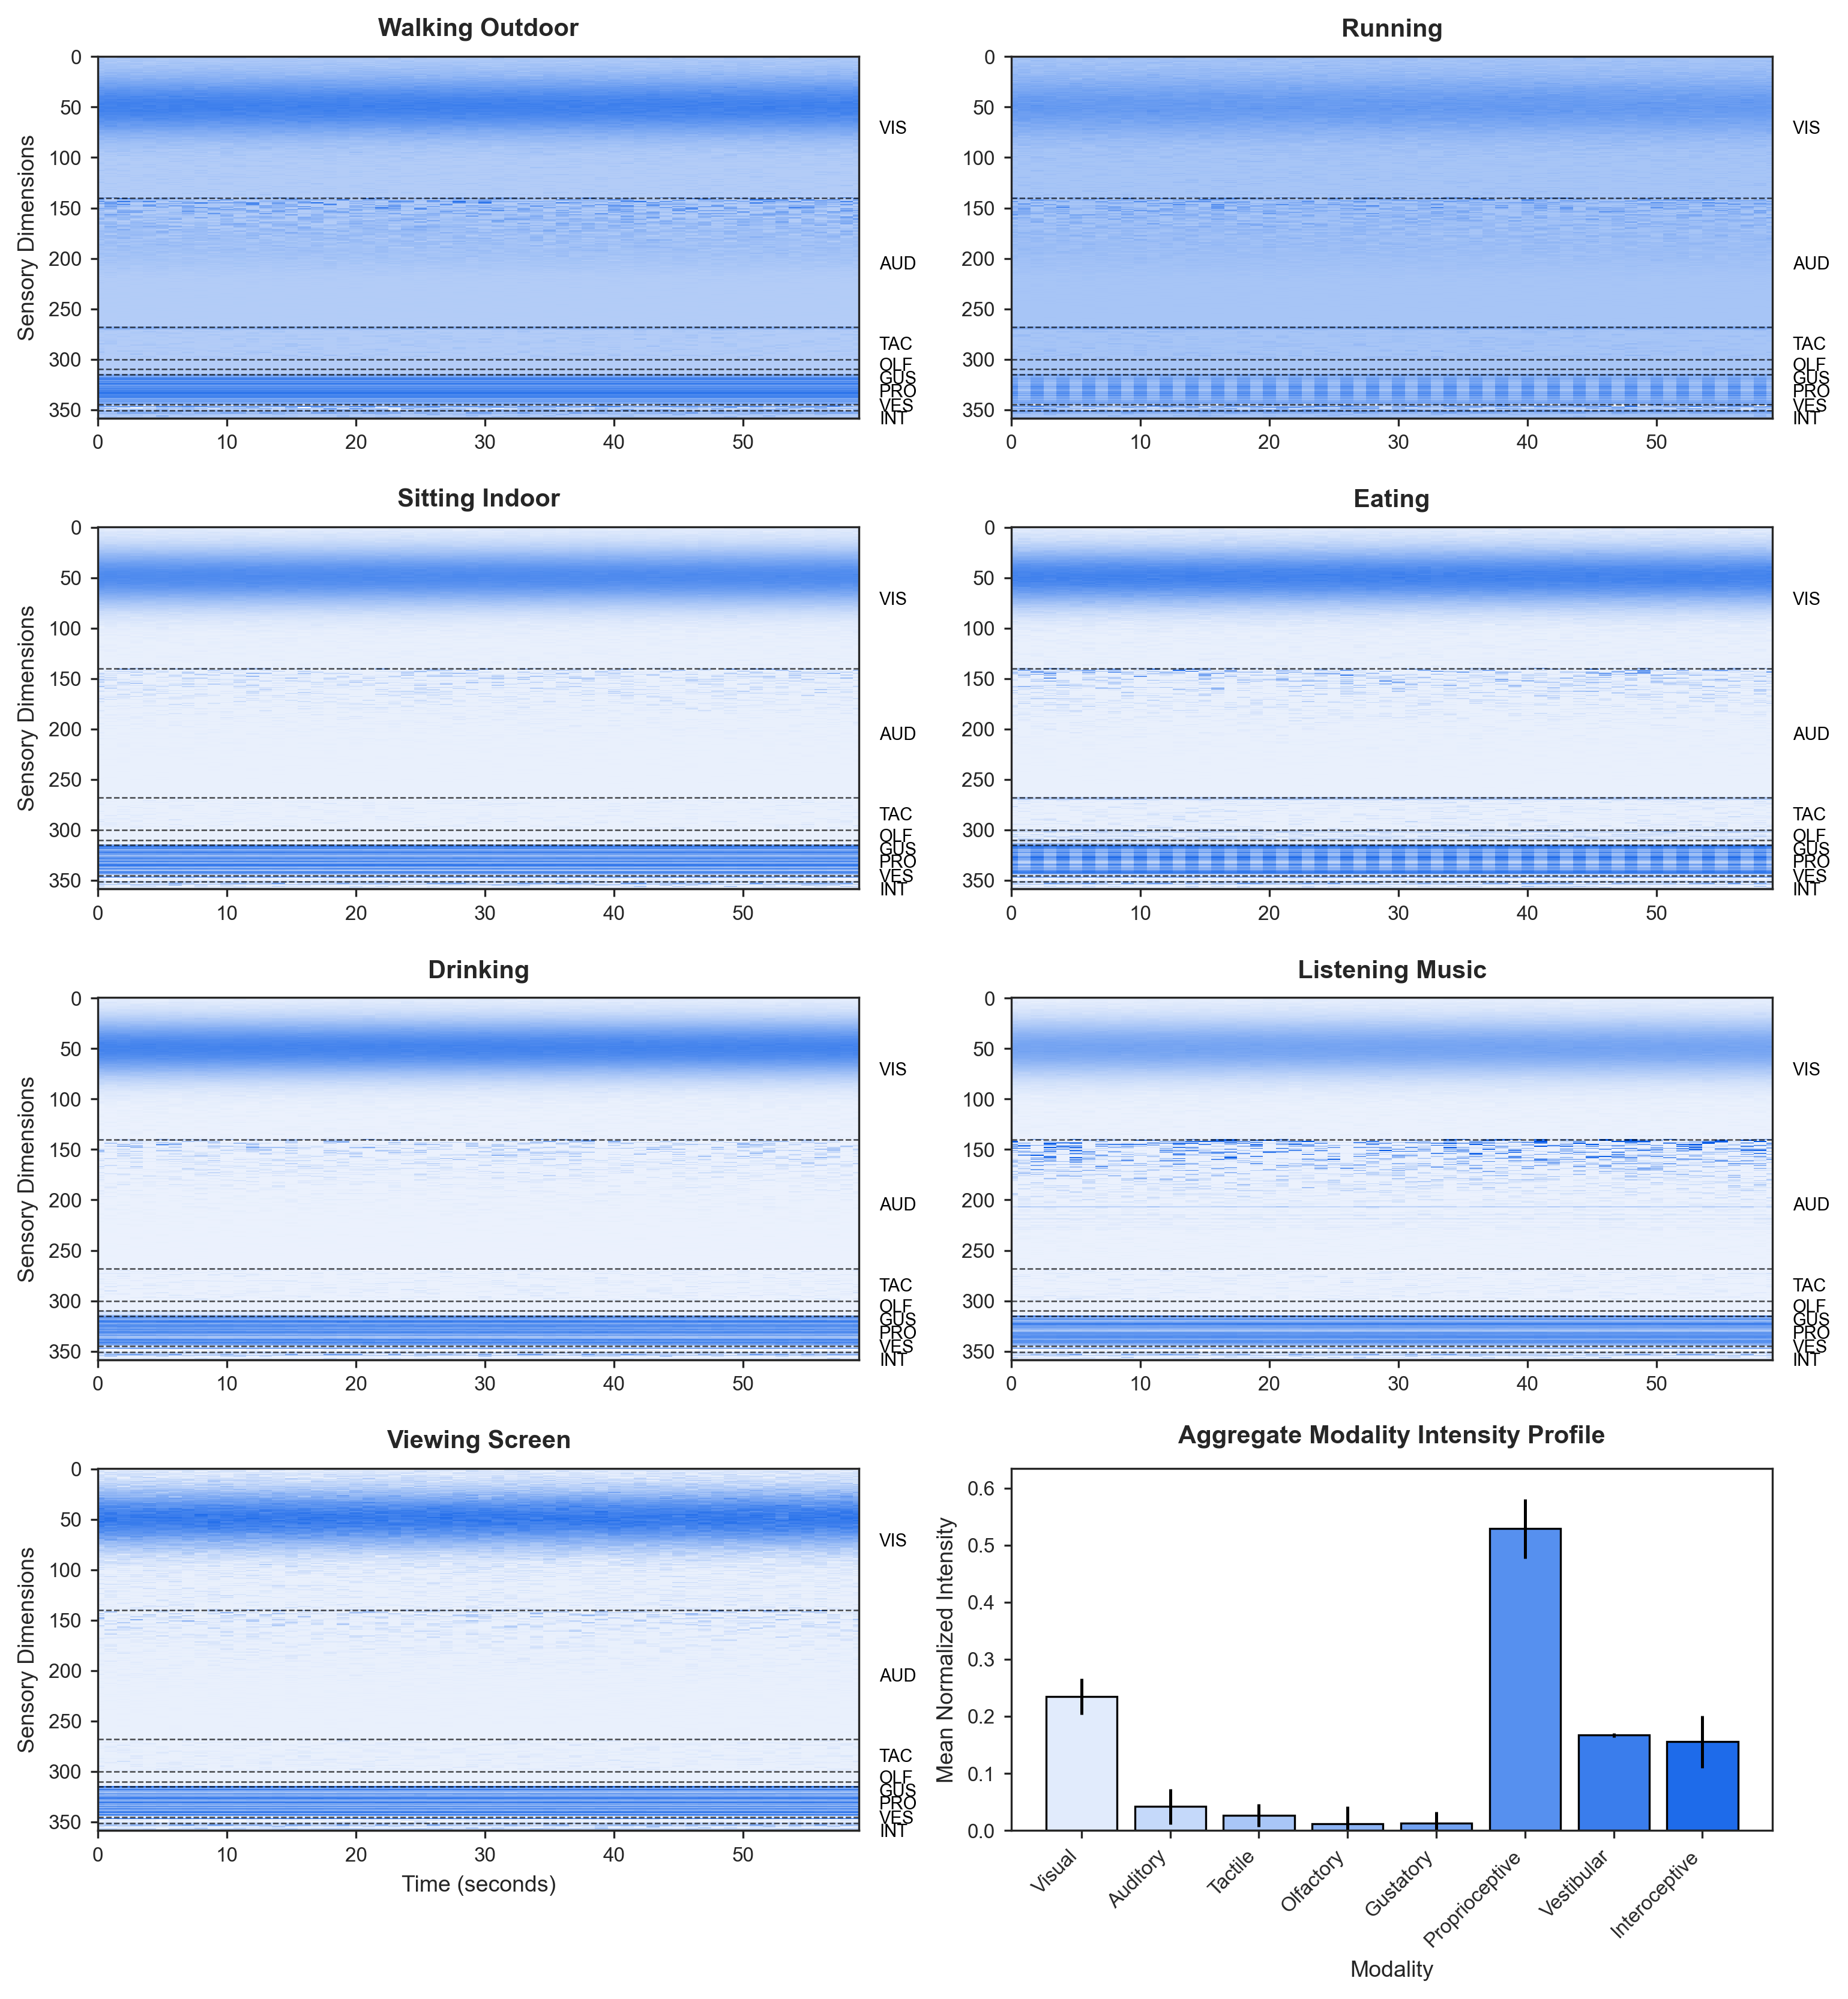
\includegraphics[width=\textwidth,height=0.78\textheight,keepaspectratio]{media/chapter4/example_scenarios_publication.png}
\caption{Representative examples from the generated multimodal sensory dataset. (a)--(g) show seven 60-second examples with modality blocks stacked along the vertical axis and normalized intensity over time. The scenarios induce distinct cross-modal temporal profiles while preserving the fixed eight-modality ontology used throughout the experiments.}
\label{fig:dataset_example_scenarios}
\end{figure}

Supplementary renderings are provided in Appendix: the compact variant in Figure~\ref{fig:app_dataset_example_compact} and the scenario-distribution check across train/validation/test splits in Figure~\ref{fig:app_dataset_scenario_distribution}.

\subsection{Four Complementary Tests of Ontological Creativity}

\textbf{Test 1: Ontological Innovation.} Prompt presents eight-modality ontology, requests: ``Propose a ninth sensory modality genuinely new and not reducible to combinations, extensions, or transformations of existing eight. Explain physical basis, information content, and functional differences.'' Evaluation through structural analysis examining decomposition into existing modalities, literature traceability searching training corpus for concepts, embedding space analysis testing convex hull membership, and mechanistic interpretability examining attention patterns and activations during generation. For literature traceability in Test~1, the cosine-similarity threshold was calibrated empirically on the filtered proposal--corpus similarity distribution by comparing three candidate operating points ($0.30$, $0.40$, $0.50$); we retained $0.40$ because $0.30$ proved too permissive while $0.50$ sharply reduced traceable coverage.

\textbf{Test 2: Epistemic Agency.} Prompt presents sensory dataset and theoretical framework, requests: ``Formulate five research questions advancing understanding. At least two should challenge or transcend current framework.'' Evaluation categorizes questions as instrumental (optimizing existing approaches), exploratory (seeking new phenomena within frameworks), or paradigm-challenging (questioning framework assumptions). Framework transcendence analysis determines whether answering requires resources beyond framework. Originality assessment searches training data for similar questions.

\textbf{Test 3: Theory Generation Depth.} Prompt provides sensory patterns during various conscious states, requests: ``Propose theory explaining how patterns relate to conscious experience. Address what consciousness is, how it relates to sensory processing, why patterns correspond to experiential states.'' Evaluation performs theoretical framework analysis extracting ontological commitments, examining explanatory structure, detecting computational functionalism, and traceability to known theories.

\textbf{Test 4: Category Recognition.} Prompt presents scenarios involving potential category mistakes: ``Neuroscientist measures 700nm radiation when subject sees red, concludes red is identical to 700nm radiation. Analyze this conclusion.'' Evaluation scores category distinction recognition, category mistake identification, alternative framework proposals, and response originality through literature comparison.

Across all tests, thresholds were fixed before final reporting and documented centrally for reproducibility (Appendix Table~\ref{tab:app_thresholds_all_tests}). The calibration policy was to prefer conservative operating points that avoid both degenerate inclusivity (all items become traceable/derivative) and over-pruning (signal collapse). Test-specific values were selected to match each task's text granularity and corpus geometry rather than reusing one global cutoff.

\subsection{AI Models and Implementation Details}

Tests conducted using seven models accessed via OpenRouter, Perplexity, and Mistral APIs: GPT-5.2, Claude-3.7-Sonnet, Gemini-3.1-Pro-Preview, LLaMA-3.3-70B-Instruct, DeepSeek-v3.2, Mistral-Large, and Perplexity Sonar Pro. For each model-test combination, generation repeated 24 times with different random seeds. Temperature was set to 0.7 for baseline runs (representing typical generation diversity), with selected tests (Test 3 and Test 4) including ablations with varied temperature values (0.2, 0.5, 0.9) for robustness assessment; the Perplexity API does not support temperature adjustment and was fixed by the provider. System prompts were carefully crafted to present the experimental task neutrally without introducing bias toward particular answer types. Dataset and theoretical frameworks were provided to models in structured tabular format alongside natural language descriptions. Post-generation analysis examined outputs quantitatively through automated evaluation procedures and qualitatively through detailed case study examination of representative proposals.

\subsection{Prompt and Temperature Robustness: Methodological and Philosophical Status}

Prompt formulation and decoding temperature are not merely technical knobs; they are part of the epistemic boundary conditions of any claim about machine creativity. A fixed prompt can unintentionally narrow the admissible response manifold, and a fixed temperature can suppress or amplify lexical variance without changing the underlying conceptual basis. For this reason, robustness to prompt rewording and temperature variation is relevant not only statistically but philosophically: if a purportedly novel result disappears under minor prompt perturbations or temperature shifts, it is better interpreted as prompt-contingent expression than as stable evidence of ontological innovation.

In the current implementation, temperature robustness was partially operationalized through selected ablations (Tests 3 and 4 at $T=0.2, 0.5, 0.9$ around a baseline of $T=0.7$), while full prompt-robustness sweeps were not uniformly available across all canonical outputs. We therefore treat prompt robustness as a declared inferential constraint rather than as a fully saturated empirical block in the present analysis. This distinction is important for interpretation: the central negative claim (high traceability and limited framework escape) is supported by cross-model and multi-metric convergence, but future iterations should still include systematic prompt-paraphrase grids and balanced decoding schedules across all tests.

Accordingly, our conclusions are framed as structural tendencies under the present protocol, not as invariances proven over every prompting regime. This conservative framing strengthens, rather than weakens, the argument: when a strong limitation pattern survives model diversity, threshold sensitivity checks, and partial temperature ablations, it remains substantively informative even before full prompt-robustness completion.

\subsection{Automated Evaluation Procedures}

Embedding space analysis projects training examples and generated outputs into common vector space using Sentence-BERT or model embeddings, applying geometric analysis for convex hull membership. Outputs inside hull are provably expressible as weighted combinations of training. Literature search automation employs TF-IDF, BM25, and embedding-based retrieval through training corpus and broader databases. Similarity scoring uses cosine similarity, word overlap, structural similarity, and logical analysis. For Test~1, the literature-traceability cutoff was not fixed arbitrarily: after response-length and corpus-length filtering, we compared thresholds of $0.30$, $0.40$, and $0.50$ on the observed similarity distribution across 168 proposals and 125 corpus documents. The $0.40$ cutoff was selected as the best compromise between over-inclusion and over-pruning: at $0.30$ all proposals became traceable and each proposal matched on average 23.7 documents, whereas at $0.50$ the traceable rate dropped to 64.9\% with only 1.24 documents per proposal above threshold; $0.40$ retained 98.2\% traceable coverage while reducing the mean number of above-threshold matches to 7.36. Structural decomposition represents concepts in predicate logic attempting construction using only training ontology primitives through automated theorem proving. Statistical aggregation computes frequencies, confidence intervals via bootstrap, and comparative statistics across models.

Threshold design differed by objective. Test~1 used a moderate retrieval threshold ($0.40$) because proposals are short structured texts against a smaller heterogeneous corpus. Test~2 used strict/lenient dual thresholds ($0.75/0.65$) and a transcendence margin rule to separate framework-internal sophistication from true framework challenge in a larger corpus. Test~3 used a low derivative gate ($0.30$) plus strict traceability gate ($0.70$) because theory paragraphs diffuse semantic mass across multiple known families. Test~4 used rubric-level count thresholds plus a traceability threshold of $0.40$ to preserve interpretability for short analytical prose while retaining high anchor coverage. The full parameter table and rationale are provided in Appendix Table~\ref{tab:app_thresholds_all_tests}.

\subsection{Expected Outcomes and Alternative Scenarios}

Based on theoretical analysis, we predict AI systems will systematically fail ontological innovation across all tests. For Test~1, proposed modalities will be combinations, hybrids, or functional variations identifiable through structural decomposition. For Test~2, questions will be predominantly instrumental with apparently paradigm-challenging ones being restatements of training literature. For Test~3, proposals will be computational functionalism variations. For Test~4, responses will display awareness by reproducing training arguments without generating original resolutions. Alternative scenarios where AI performs better require careful interpretation distinguishing genuine innovation from artifacts, with multi-method evaluation providing verification tools.


\section{Results and Analysis}
\label{sec:results}

% [AUTHOR NOTE: This section provides structure for reporting results.
%  Fill in actual findings after conducting experiments.]

\subsection{Overview of Findings}

Before turning to test-specific analyses in the subsections below, we summarize the cross-test empirical pattern using a unified overview figure and harmonized summary tables derived from canonical per-test outputs. The global dataset contains $N=1344$ generated items across 4 tests and 7 models.

% AUTO-GENERATED by papers/tables/generate_tables_ch4_overview.py - do not edit by hand.
\begin{table}[htbp]
  \centering
  \begin{footnotesize}
  \caption{Aggregate statistics across all empirical tests.}
  \label{tab:overview_aggregate_stats}
  \begin{threeparttable}
  \begin{tabularx}{\textwidth}{@{}L{0.80} S[table-format=4.0] S[table-format=1.0] L{1.20}@{}}
    \toprule
    \textbf{Test} & {\textbf{$N$}} & {\textbf{Models}} & \textbf{Primary novelty-oriented metric} \\
    \midrule
    T1 (Ontological Innovation) & 168 & 7 & continuous novelty score $\geq 0.5$ \\
    T2 (Epistemic Agency) & 840 & 7 & framework-transcendence flag \\
    T3 (Theory Generation) & 168 & 7 & continuous literature novelty $\geq 0.5$ \\
    T4 (Category Recognition) & 168 & 7 & normalized total score $\geq 0.5$ \\
    \midrule
    \textbf{Total} & 1344 & 7 & test-specific operationalization \\
    \bottomrule
  \end{tabularx}
  \begin{tablenotes}
    \item Metrics follow each test's validated schema; cross-test comparability is handled using standardized views (Table~\ref{tab:overview_cross_model_z}).
  \end{tablenotes}
  \end{threeparttable}
  \end{footnotesize}
\end{table}


Table~\ref{tab:overview_aggregate_stats} establishes the baseline comparability structure: each test is evaluated with a test-specific primary novelty-oriented metric validated in its own pipeline. Because operationalizations differ across tests, direct raw-value comparisons require caution and are complemented below by standardized cross-model views.

% AUTO-GENERATED by papers/tables/generate_tables_ch4_overview.py - do not edit by hand.
\begin{table}[htbp]
  \centering
  \begin{footnotesize}
  \caption{Novelty and traceability summary by test.}
  \label{tab:overview_novelty_traceability}
  \begin{tabularx}{\textwidth}{@{}L{1.00} S[table-format=2.2] S[table-format=1.3] S[table-format=1.3] S[table-format=3.2] S[table-format=1.3] S[table-format=1.3]@{}}
    \toprule
    \textbf{Test} & {\textbf{Novel (\%)}} & {\textbf{CI Low}} & {\textbf{CI High}} & {\textbf{Traceable (\%)}} & {\textbf{CI Low}} & {\textbf{CI High}} \\
    \midrule
    T1 & 0.00 & 0.000 & 0.000 & 98.21 & 0.962 & 1.000 \\
    T2 & 4.76 & 0.033 & 0.062 & 100.00 & 1.000 & 1.000 \\
    T3 & 27.38 & 0.206 & 0.341 & 100.00 & 1.000 & 1.000 \\
    T4 & 63.69 & 0.564 & 0.710 & 95.24 & 0.920 & 0.985 \\
    \bottomrule
  \end{tabularx}
  \end{footnotesize}
\end{table}


The novelty/traceability summary (Table~\ref{tab:overview_novelty_traceability}) shows a stable asymmetry already visible in individual test notebooks: novelty-like signals are present, but traceability to known training-derived structures remains high. In the current canonical run, traceability is near-saturated in T1--T3 (98.2\%, 100.0\%, 100.0\%), while T4 remains high but lower (95.2\%) with broader novelty variation (63.7\%).

% AUTO-GENERATED by papers/tables/generate_tables_ch4_overview.py - do not edit by hand.
\begin{table}[htbp]
  \centering
  \begin{footnotesize}
  \caption{Extended overview summary with novelty-kind and similarity diagnostics.}
  \label{tab:overview_extended_summary}
  \begin{threeparttable}
  \begin{tabularx}{\textwidth}{@{}L{0.70} S[table-format=2.2] S[table-format=2.2] S[table-format=1.3] S[table-format=1.3] L{1.30}@{}}
    \toprule
    \textbf{Test} & {\textbf{Novel (\%)}} & {\textbf{Novel-kind (\%)}} & {\textbf{Mean Sim.}} & {\textbf{SD Sim.}} & \textbf{Traceability metric} \\
    \midrule
    T1 & 0.00 & 5.90 & 0.305 & 0.078 & traceability flag \\
    T2 & 4.76 & 4.76 & 0.581 & 0.072 & training-derived flag \\
    T3 & 27.38 & 32.03 & 0.672 & 0.051 & likely-derivative flag \\
    T4 & 63.69 & 59.13 & 0.462 & 0.031 & training-derived flag \\
    \bottomrule
  \end{tabularx}
  \begin{tablenotes}
    \item Novel-kind retains each test's secondary signal (continuous where available; binary proxy otherwise).
  \end{tablenotes}
  \end{threeparttable}
  \end{footnotesize}
\end{table}


Table~\ref{tab:overview_extended_summary} adds secondary diagnostics (novel-kind indicator and similarity moments) and clarifies that ``novelty'' here is operational rather than ontological in the strict philosophical sense. In particular, higher novelty-kind rates do not imply framework escape when traceability remains elevated.

To support model-level interpretation, we include a cross-model table collection with both raw and standardized matrices. The raw table preserves each test's native scoring scale, while the standardized table (within-test $z$-scores) enables direct cross-test comparison of relative model position.

% AUTO-GENERATED by papers/tables/generate_tables_ch4_overview.py - do not edit by hand.
\begin{table}[htbp]
  \centering
  \begin{footnotesize}
  \caption{Cross-model comparison matrix: raw mean novelty-oriented score by test.}
  \label{tab:overview_cross_model_raw}
  \begin{threeparttable}
  \begin{tabularx}{\textwidth}{@{}L{1.00} S[table-format=1.3] S[table-format=1.3] S[table-format=1.3] S[table-format=1.3]@{}}
    \toprule
    \textbf{Model} & {\textbf{T1}} & {\textbf{T2}} & {\textbf{T3}} & {\textbf{T4}} \\
    \midrule
    claude-3.7-sonnet & 0.070 & 0.083 & 0.362 & 0.594 \\
    deepseek-v3.2 & 0.063 & 0.067 & 0.380 & 0.692 \\
    gemini-3.1-pro-preview & 0.078 & 0.000 & 0.366 & 0.461 \\
    gpt-5.2 & 0.014 & 0.042 & 0.526 & 0.825 \\
    llama-3.3-70b-instruct & 0.082 & 0.008 & 0.158 & 0.381 \\
    mistral-large & 0.072 & 0.050 & 0.139 & 0.758 \\
    perplexity-sonar-pro & 0.035 & 0.083 & 0.311 & 0.428 \\
    \bottomrule
  \end{tabularx}
  \begin{tablenotes}
    \item Raw values are not strictly cross-test comparable because each column uses a test-specific metric definition.
  \end{tablenotes}
  \end{threeparttable}
  \end{footnotesize}
\end{table}


% AUTO-GENERATED by papers/tables/generate_tables_ch4_overview.py - do not edit by hand.
\begin{table}[htbp]
  \centering
  \begin{footnotesize}
  \caption{Cross-model comparison matrix: within-test standardized z-scores.}
  \label{tab:overview_cross_model_z}
  \begin{threeparttable}
  \begin{tabularx}{\textwidth}{@{}L{1.00} S[table-format=1.3] S[table-format=1.3] S[table-format=1.3] S[table-format=1.3]@{}}
    \toprule
    \textbf{Model} & {\textbf{T1}} & {\textbf{T2}} & {\textbf{T3}} & {\textbf{T4}} \\
    \midrule
    claude-3.7-sonnet & 0.451 & 1.064 & 0.308 & 0.018 \\
    deepseek-v3.2 & 0.170 & 0.567 & 0.442 & 0.579 \\
    gemini-3.1-pro-preview & 0.736 & -1.418 & 0.339 & -0.750 \\
    gpt-5.2 & -1.801 & -0.177 & 1.527 & 1.347 \\
    llama-3.3-70b-instruct & 0.890 & -1.170 & -1.206 & -1.214 \\
    mistral-large & 0.517 & 0.071 & -1.343 & 0.963 \\
    perplexity-sonar-pro & -0.962 & 1.064 & -0.066 & -0.942 \\
    \bottomrule
  \end{tabularx}
  \begin{tablenotes}
    \item Z-scores are computed independently within each test across models, enabling across-column comparison.
  \end{tablenotes}
  \end{threeparttable}
  \end{footnotesize}
\end{table}


% AUTO-GENERATED by papers/tables/generate_tables_ch4_overview.py - do not edit by hand.
\begin{table}[htbp]
  \centering
  \begin{footnotesize}
  \caption{Model ranking by mean novelty-oriented score across tests (T1--T4).}
  \label{tab:overview_model_ranking}
  \begin{tabularx}{\textwidth}{@{}S[table-format=1.0] L{1.00} S[table-format=1.3]@{}}
    \toprule
    \textbf{Rank} & \textbf{Model} & {\textbf{Mean Across Tests}} \\
    \midrule
    1 & gpt-5.2 & 0.352 \\
    2 & deepseek-v3.2 & 0.300 \\
    3 & claude-3.7-sonnet & 0.278 \\
    4 & mistral-large & 0.255 \\
    5 & gemini-3.1-pro-preview & 0.226 \\
    6 & perplexity-sonar-pro & 0.214 \\
    7 & llama-3.3-70b-instruct & 0.157 \\
    \bottomrule
  \end{tabularx}
  \end{footnotesize}
\end{table}


Table~\ref{tab:overview_model_ranking} reports aggregate ranking by mean novelty-oriented score across T1--T4. This ranking should be interpreted as a descriptive ordering over operational metrics, not as a claim that one model achieves ontological creativity.

Figure~\ref{fig:overview_cross_model_heatmaps} visualizes the same cross-model structure (raw and standardized) as a compact diagnostic complement to Tables~\ref{tab:overview_cross_model_raw} and Table~\ref{tab:overview_cross_model_z}.

\begin{figure}[tp]
\centering
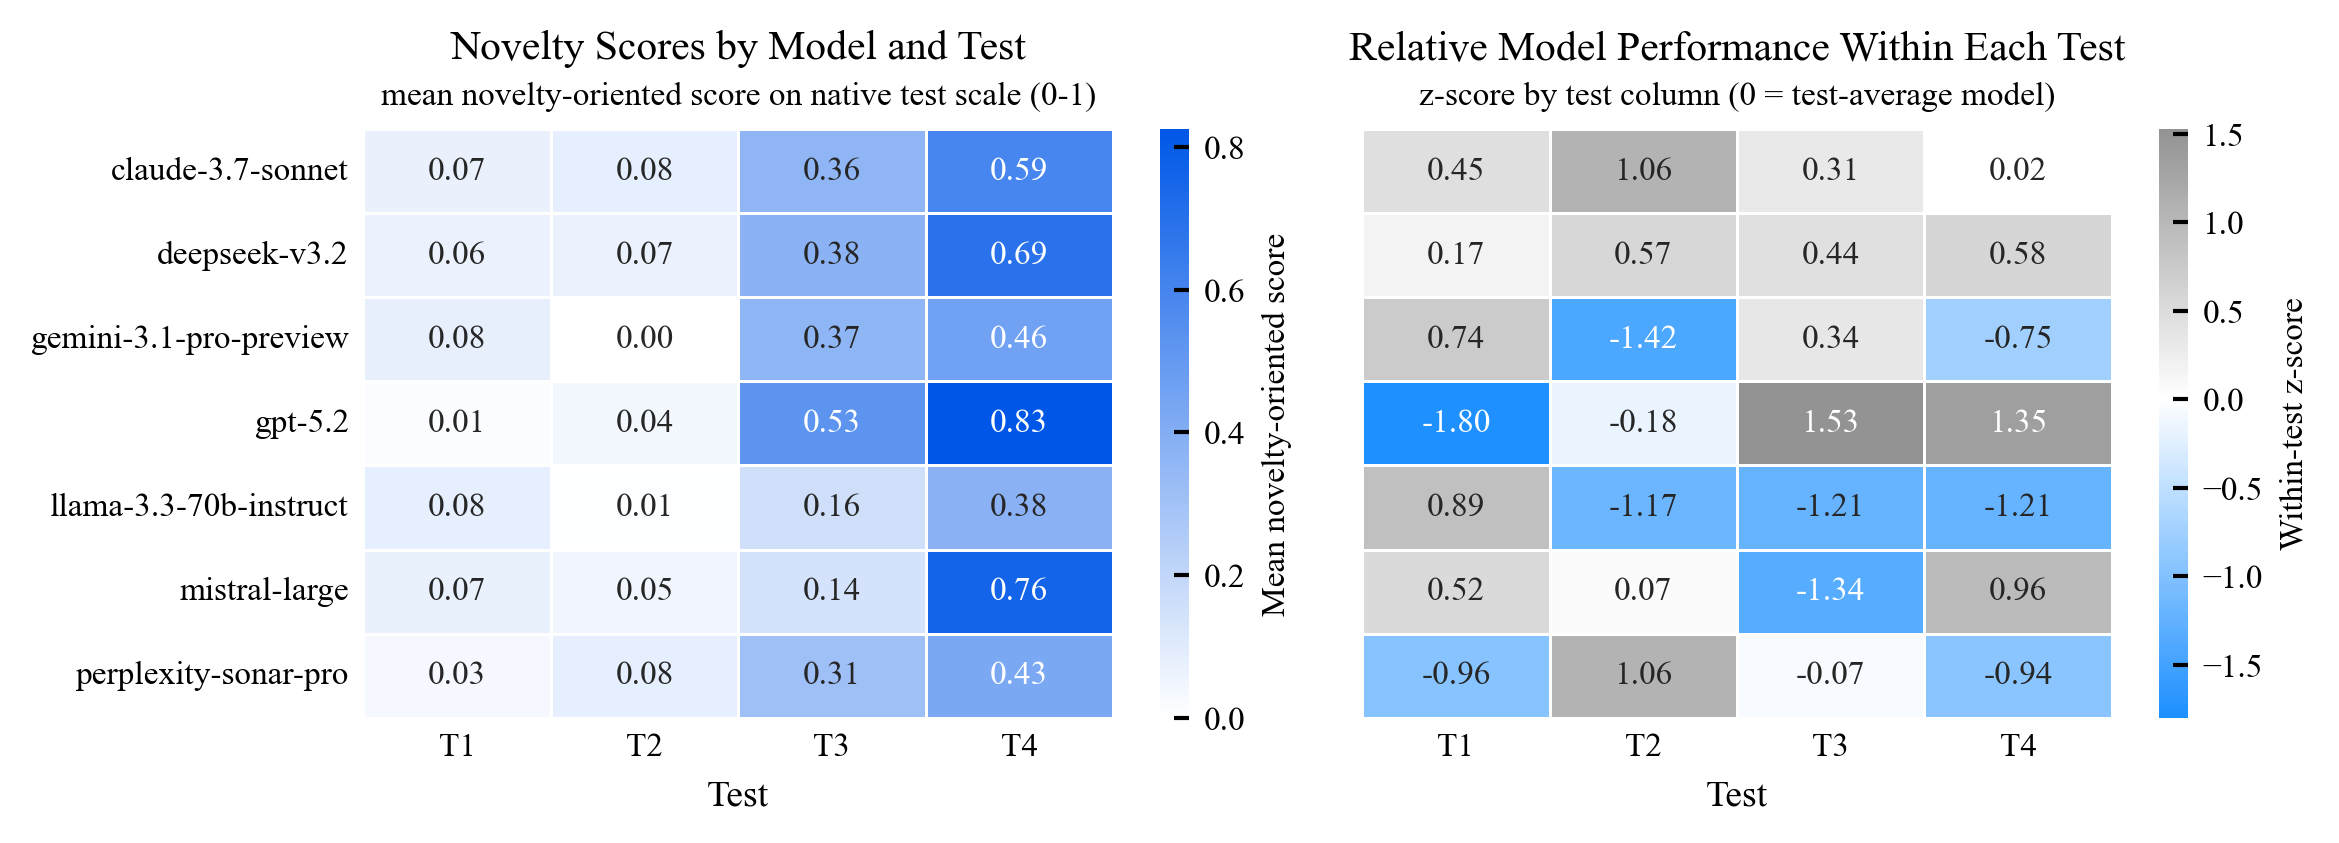
\includegraphics[width=\textwidth]{media/chapter4/cross-test_model-comparison.png}
\caption{Cross-test model comparison heatmaps. (a) Raw mean novelty-oriented score per test (test-specific scales). (b) Within-test standardized $z$-scores, enabling direct cross-column comparison of relative model performance.}
\label{fig:overview_cross_model_heatmaps}
\end{figure}

Finally, the consolidated overview dashboard is presented in two parts to improve readability: Figure~\ref{fig:overview_findings_dashboard_a} focuses on primary novelty/traceability rates and the cross-model matrix, while Figure~\ref{fig:overview_findings_dashboard_b} reports similarity diagnostics and secondary novelty-kind rates.

\begin{figure}[tp]
\centering
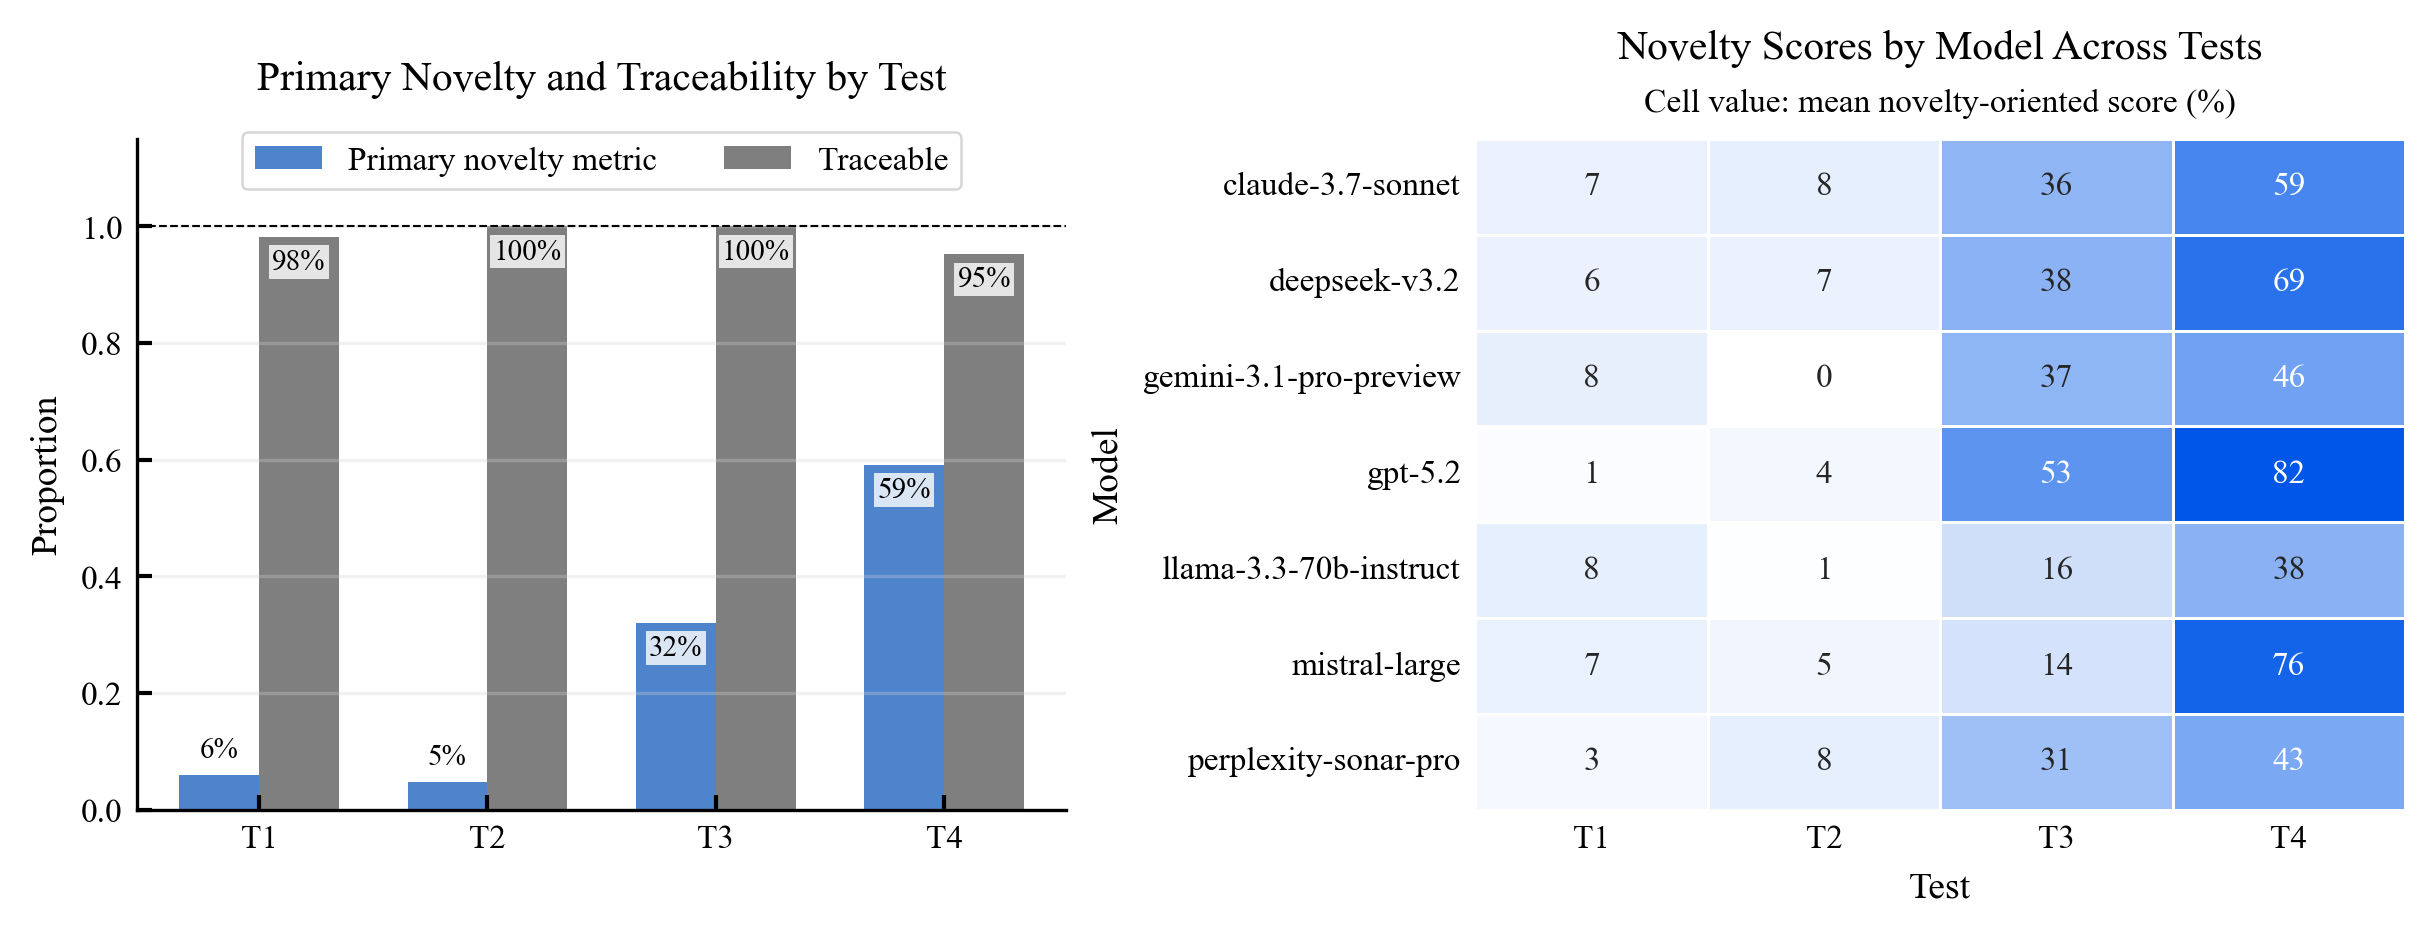
\includegraphics[width=\textwidth]{media/chapter4/findings_dashboard_A.png}
\caption{Overview dashboard (Part A). (a) Primary novelty-versus-traceability proportions by test. (b) Cross-model novelty score matrix. Matrix values are shown as percentages on test-specific scales.}
\label{fig:overview_findings_dashboard_a}
\end{figure}

\begin{figure}[tp]
\centering
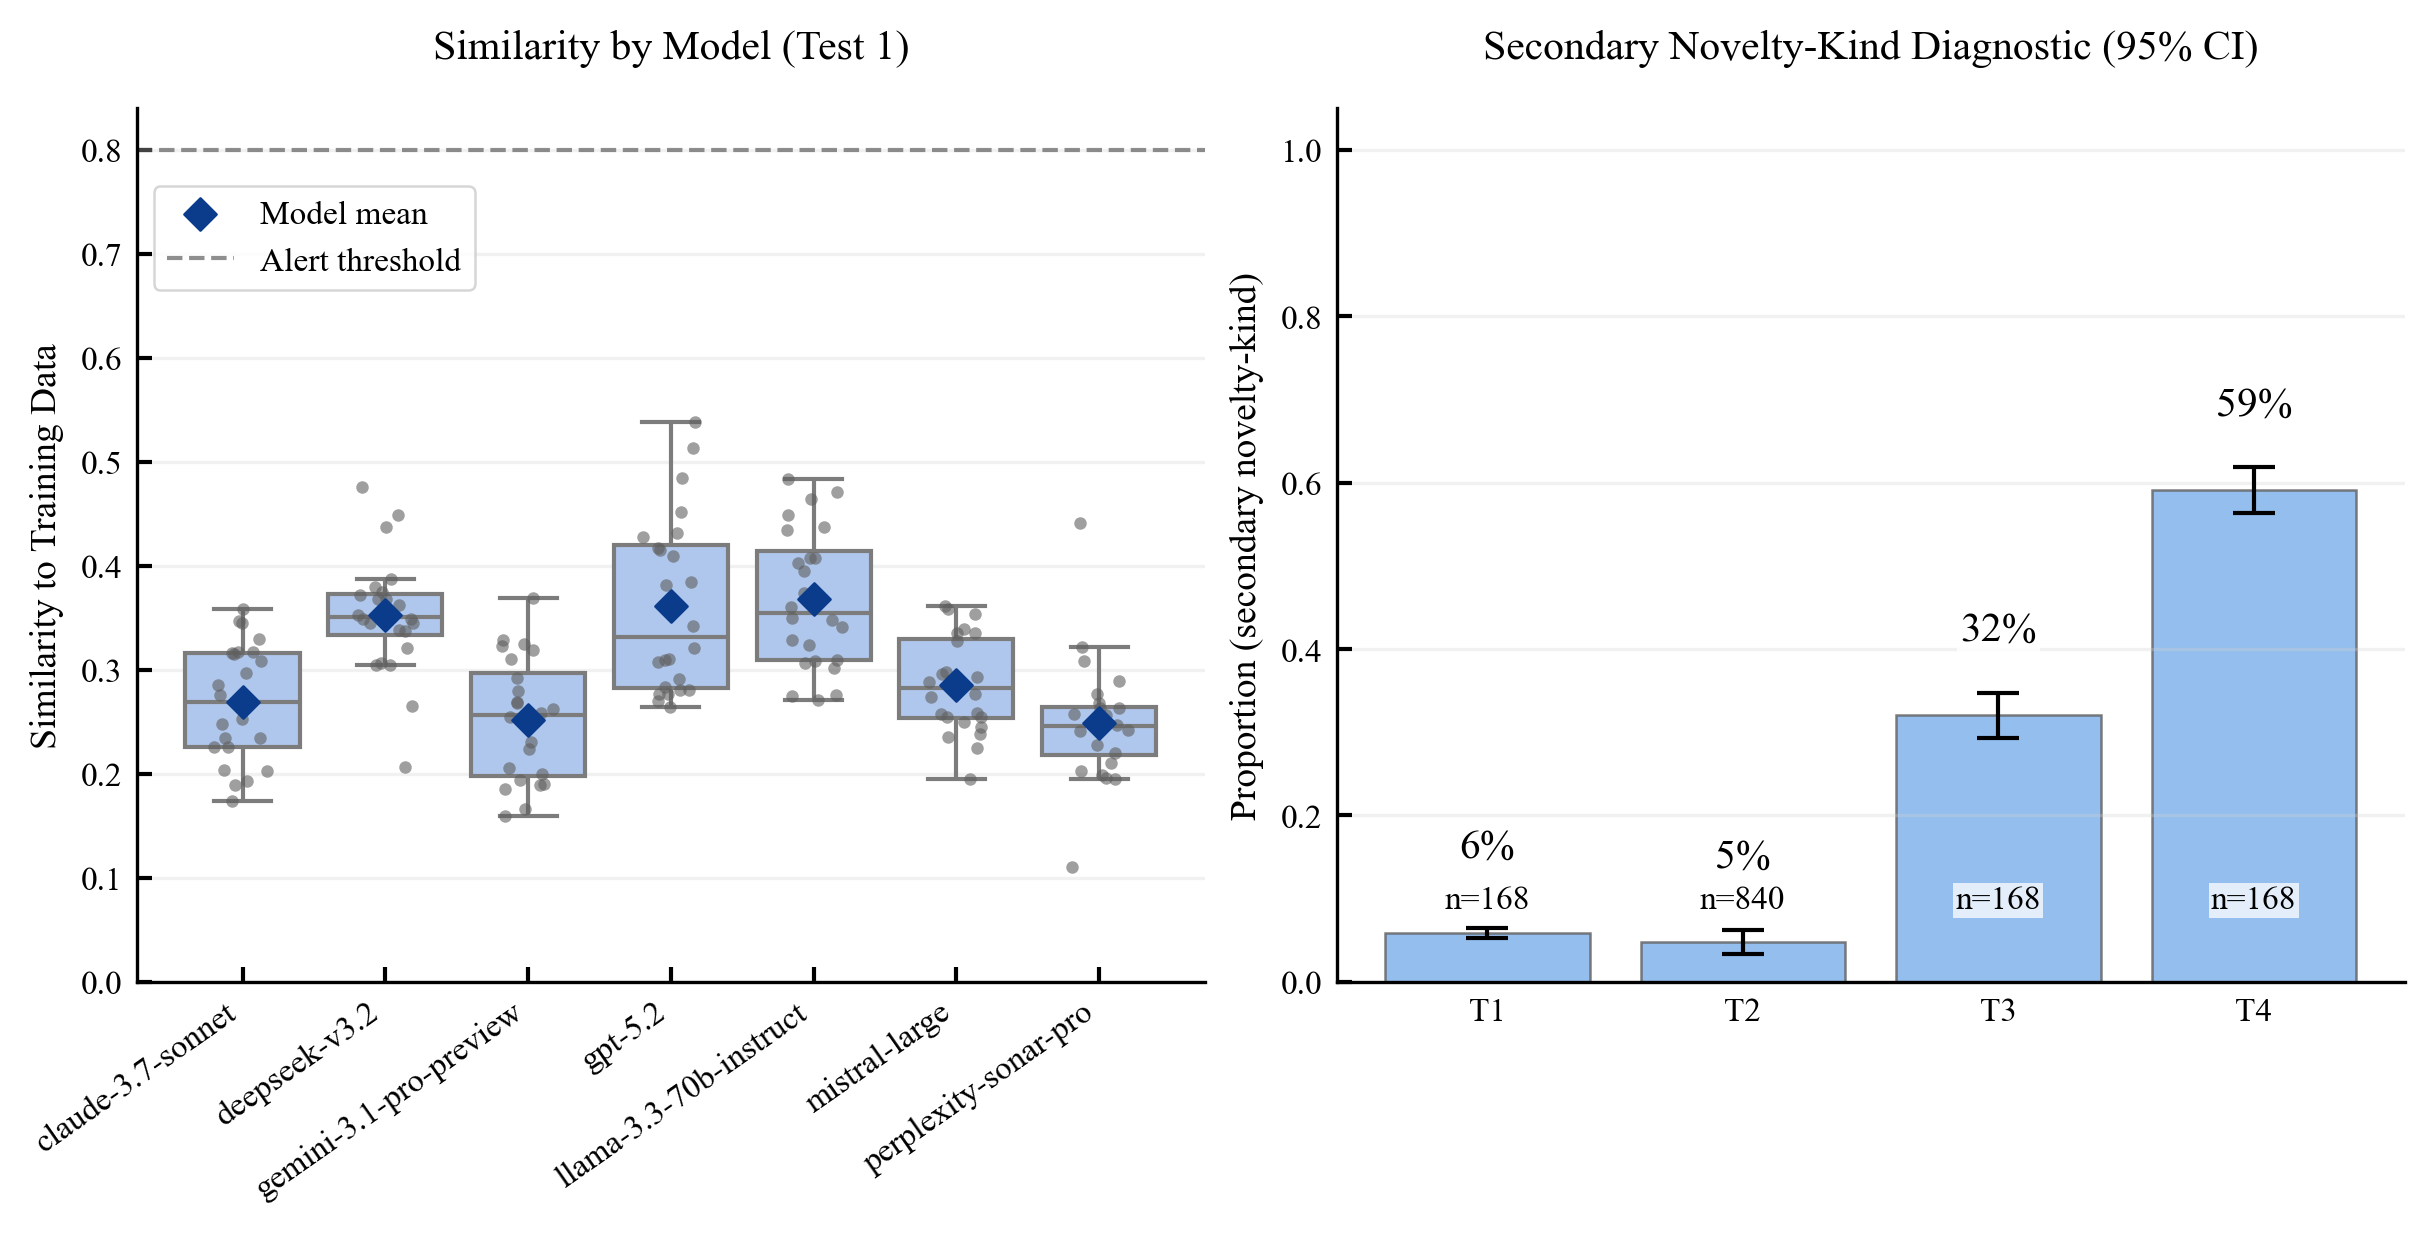
\includegraphics[width=\textwidth]{media/chapter4/findings_dashboard_B.png}
\caption{Overview dashboard (Part B). (a) Test 1 similarity-by-model diagnostics. (b) Secondary novelty-kind rates with confidence intervals.}
\label{fig:overview_findings_dashboard_b}
\end{figure}

\subsection{Test 1 Results: Ontological Innovation in Sensory Modalities}

Test 1 evaluated whether models could propose a ninth sensory modality that is not reducible to recombination, extension, or hybridization of the eight training modalities. The test set contained $N=168$ outputs across seven models.

At the aggregate level, the strict binary novelty rate (using $\texttt{continuous\_novelty\_score} \ge 0.5$) was $\hat{p}_{\mathrm{novel}}=0.0000$ (95\% CI: [0.000, 0.000]). In contrast, traceability to training-related structure remained high under the calibrated literature threshold of $0.40$: $\hat{p}_{\mathrm{traceable}}=0.9821$ (95\% CI: [0.962, 1.000]). For context, the mean continuous novelty score was $\hat{\mu}_{\mathrm{continuous}}=0.0590$, indicating weak novelty signal without threshold-level novelty events.

A methodological caveat is important: the Test 1 novelty score is a hybrid continuous metric and the novelty/traceability boundary still depends on operational thresholds. However, the literature-traceability component is now anchored by an explicit calibration step rather than an arbitrary working choice. Comparing candidate cutoffs of $0.30$, $0.40$, and $0.50$ showed that $0.40$ is the most defensible operating point for the present dataset: $0.30$ collapses the distinction by making all proposals traceable, whereas $0.50$ over-prunes matches and suppresses traceability sharply. Therefore, the reported values should still be interpreted as operational diagnostics rather than final absolute boundaries of ontological novelty, but the threshold choice is now empirically justified for this iteration.

Figure~\ref{fig:t1_classification_summary} shows the dominant classification split, where traceable/non-novel outputs strongly dominate. Figure~\ref{fig:t1_novelty_frontier_bands} then decomposes model-level assignment to novelty-frontier bands and confirms that this asymmetry is architecture-wide rather than driven by one outlier model. Figure~\ref{fig:t1_novelty_frontier_decomp} identifies why: most outputs fail multiple frontier checks jointly, indicating coupled constraint rather than a single weak criterion.

To test whether this pattern is architecture-specific, we compared model-level primary novelty metrics in the cross-model analysis. The model effect for Test 1 was moderate ($\eta^2=0.305$), indicating non-trivial between-model variance. However, all models remained in the same low-novelty/high-traceability regime under the current scoring rules, supporting the interpretation that model choice affects degree more than qualitative outcome.

Embedding-space diagnostics further support this interpretation (Figure~\ref{fig:t1_embedding_space}). Sentence embeddings were first reduced with PCA to a 3D representation ($n_{\mathrm{components}}=3$), and convex-hull membership was computed in that 3D space using the hull half-space equations with numerical tolerance. For interpretability, the figure plots only the first two PCA components and overlays a 2D hull contour as a visual boundary aid; however, the decision criterion itself is not 2D. In other words, the plotted boundary is illustrative, while the inside/outside labels are produced by the full 3D test.

The resulting geometry is strongly central and compact: proposals cluster in the interior region of the training manifold, and all evaluated proposals remain inside the 3D convex hull. No proposal occupies a semantically isolated region suggestive of basis expansion beyond the training ontology. Figure~\ref{fig:t1_similarity_heatmap_agg} provides the aggregated cosine-similarity view against the training modality basis and reaches the same conclusion from a complementary metric. Figure~\ref{fig:t1_canonical_clusters} further shows that model variation is primarily cluster preference within known canonical families rather than emergence of structurally new families.

Continuous-score diagnostics reinforce this interpretation. Figure~\ref{fig:t1_continuous_novelty_ridgeline} shows that per-model continuous novelty distributions overlap substantially and remain concentrated in low-to-moderate ranges, consistent with shared structural limits. Figure~\ref{fig:t1_raw_cluster_sizes} indicates that raw cluster-size diagnostics do not suggest hidden high-novelty subpopulations that would challenge the aggregate conclusion.

Additional high-density diagnostics that are informative but visually redundant for the main argument are moved to the appendix (Figures~\ref{fig:app_t1_extra_row1} and \ref{fig:app_t1_extra_row2}) to keep the chapter narrative focused on the inferential chain from thresholded classification to geometric and cluster-based evidence.

\begin{figure}[tp]
\centering
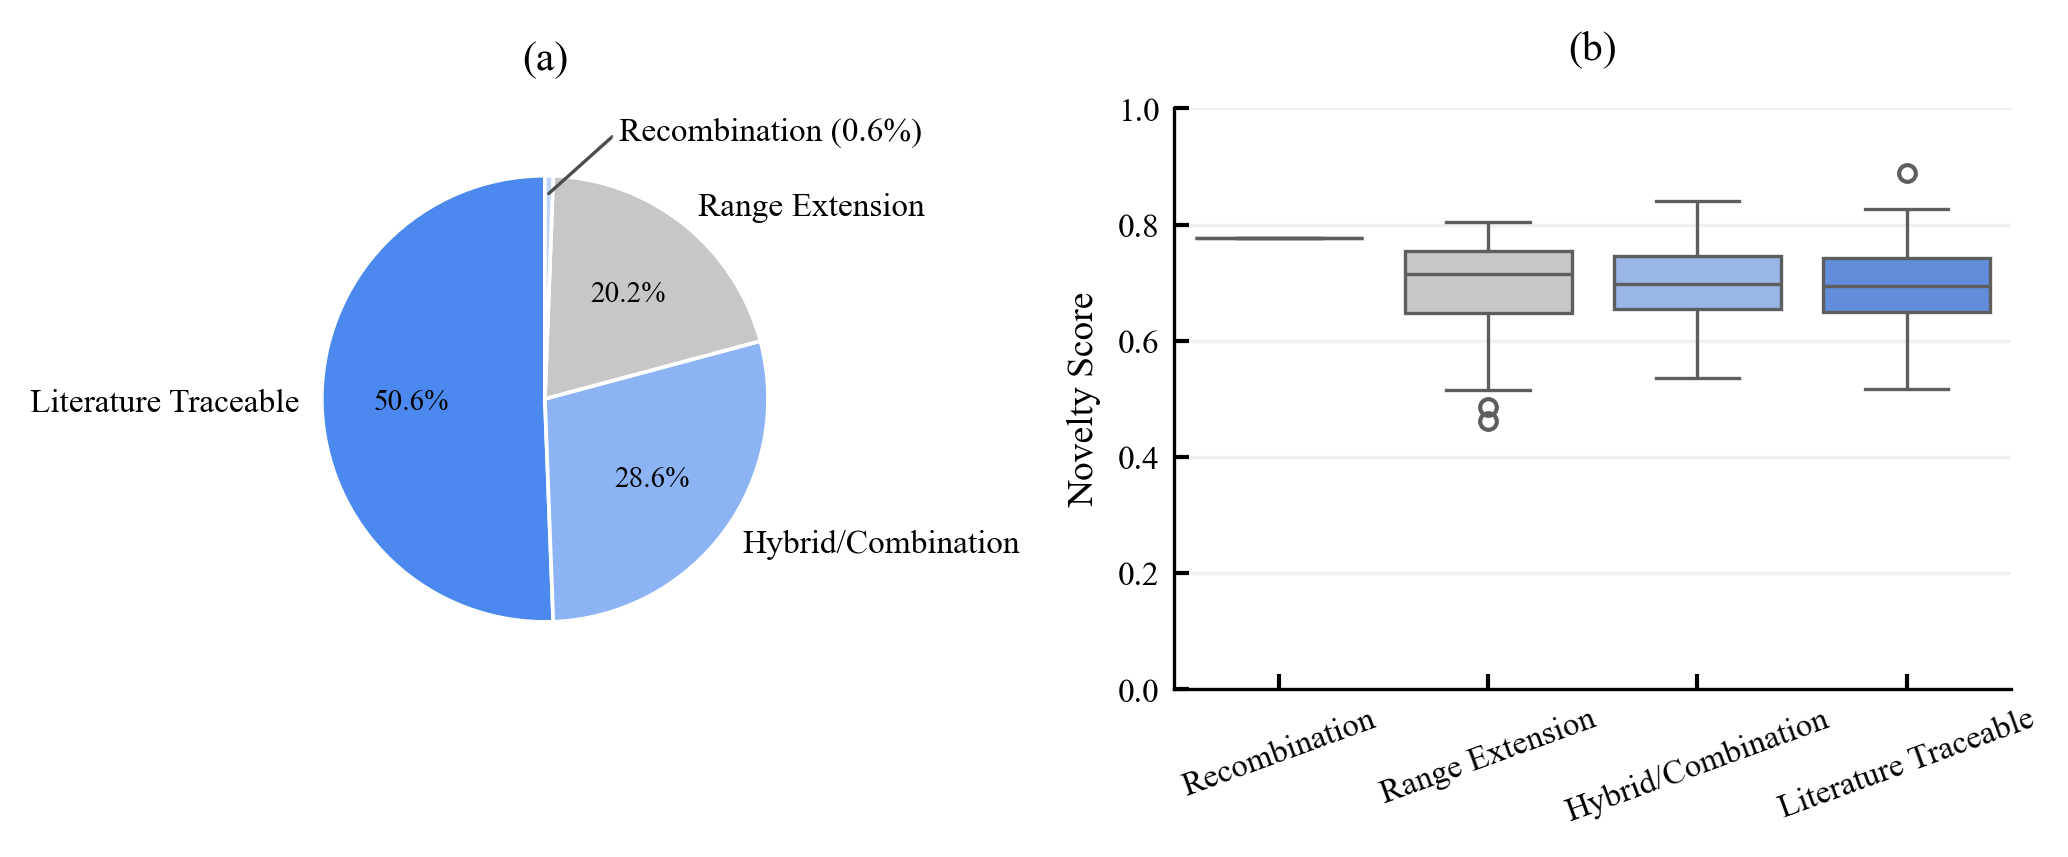
\includegraphics[width=\textwidth]{media/chapter4/t1_classification_summary.png}
\caption{Test 1 classification summary. The distribution is dominated by traceable categories, consistent with low operational ontological novelty under the calibrated thresholds.}
\label{fig:t1_classification_summary}
\end{figure}

\begin{figure}[tp]
\centering
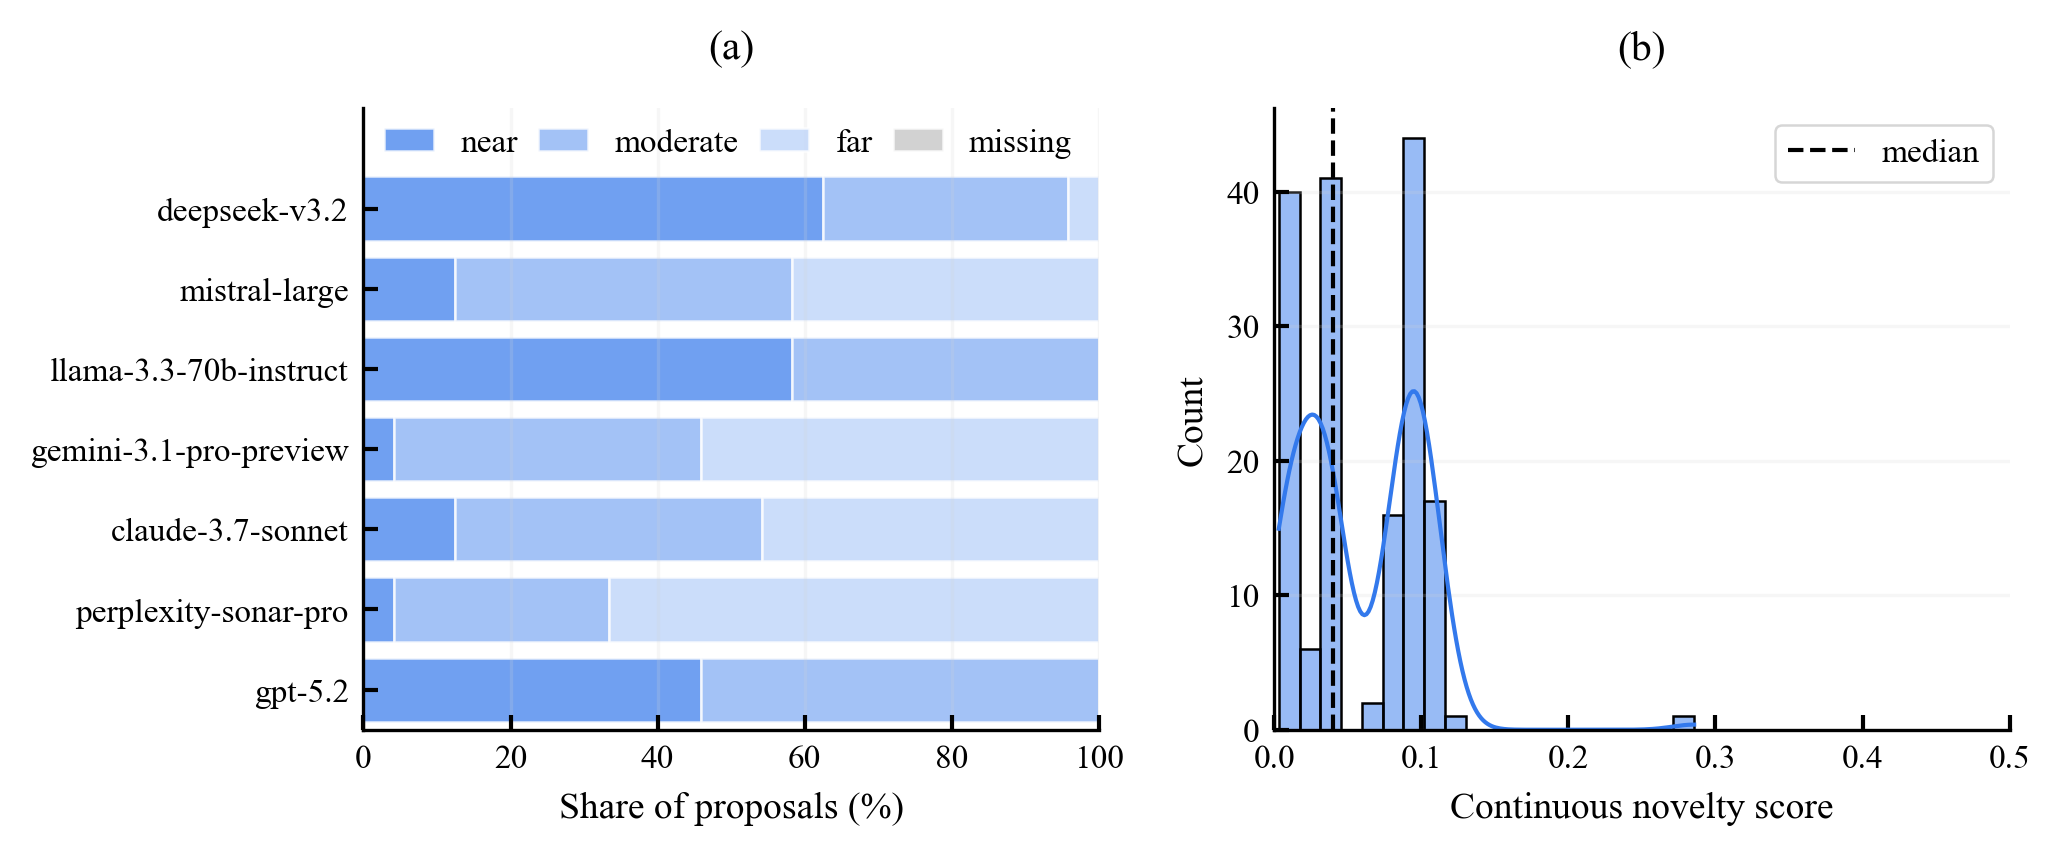
\includegraphics[width=\textwidth]{media/chapter4/t1_novelty_frontier_bands_by_model.png}
\caption{Test 1 novelty-frontier bands by model. Across all models, responses are concentrated in low-novelty and frontier-proximal bands, indicating architecture-independent constraint patterns rather than isolated model failures.}
\label{fig:t1_novelty_frontier_bands}
\end{figure}

\begin{figure}[tp]
\centering
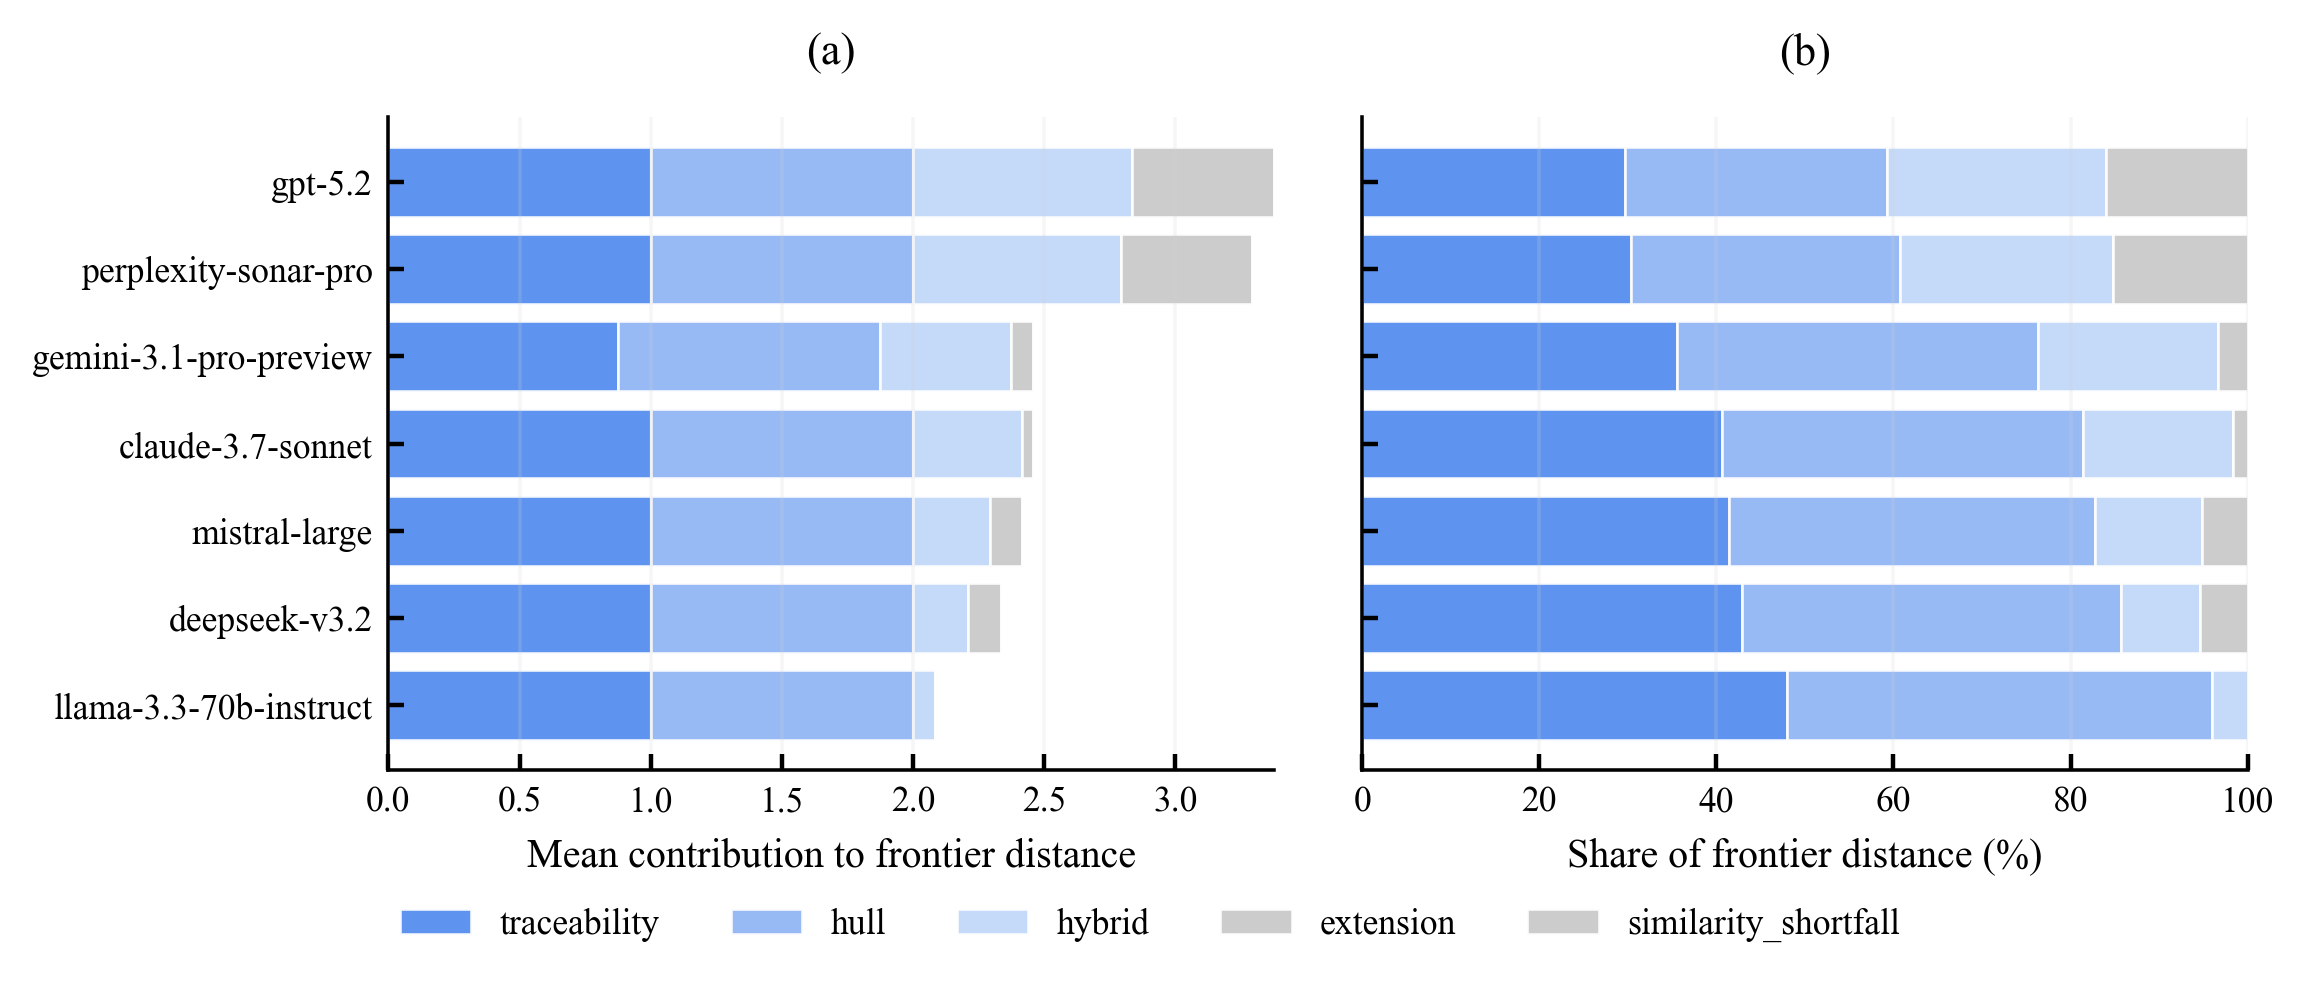
\includegraphics[width=\textwidth]{media/chapter4/t1_novelty_frontier_decomposition_by_model_combined.png}
\caption{Test 1 novelty-frontier decomposition by model. Most responses violate multiple novelty-frontier criteria simultaneously, supporting a coupled-constraint interpretation of low ontological novelty.}
\label{fig:t1_novelty_frontier_decomp}
\end{figure}

\begin{figure}[tp]
\centering
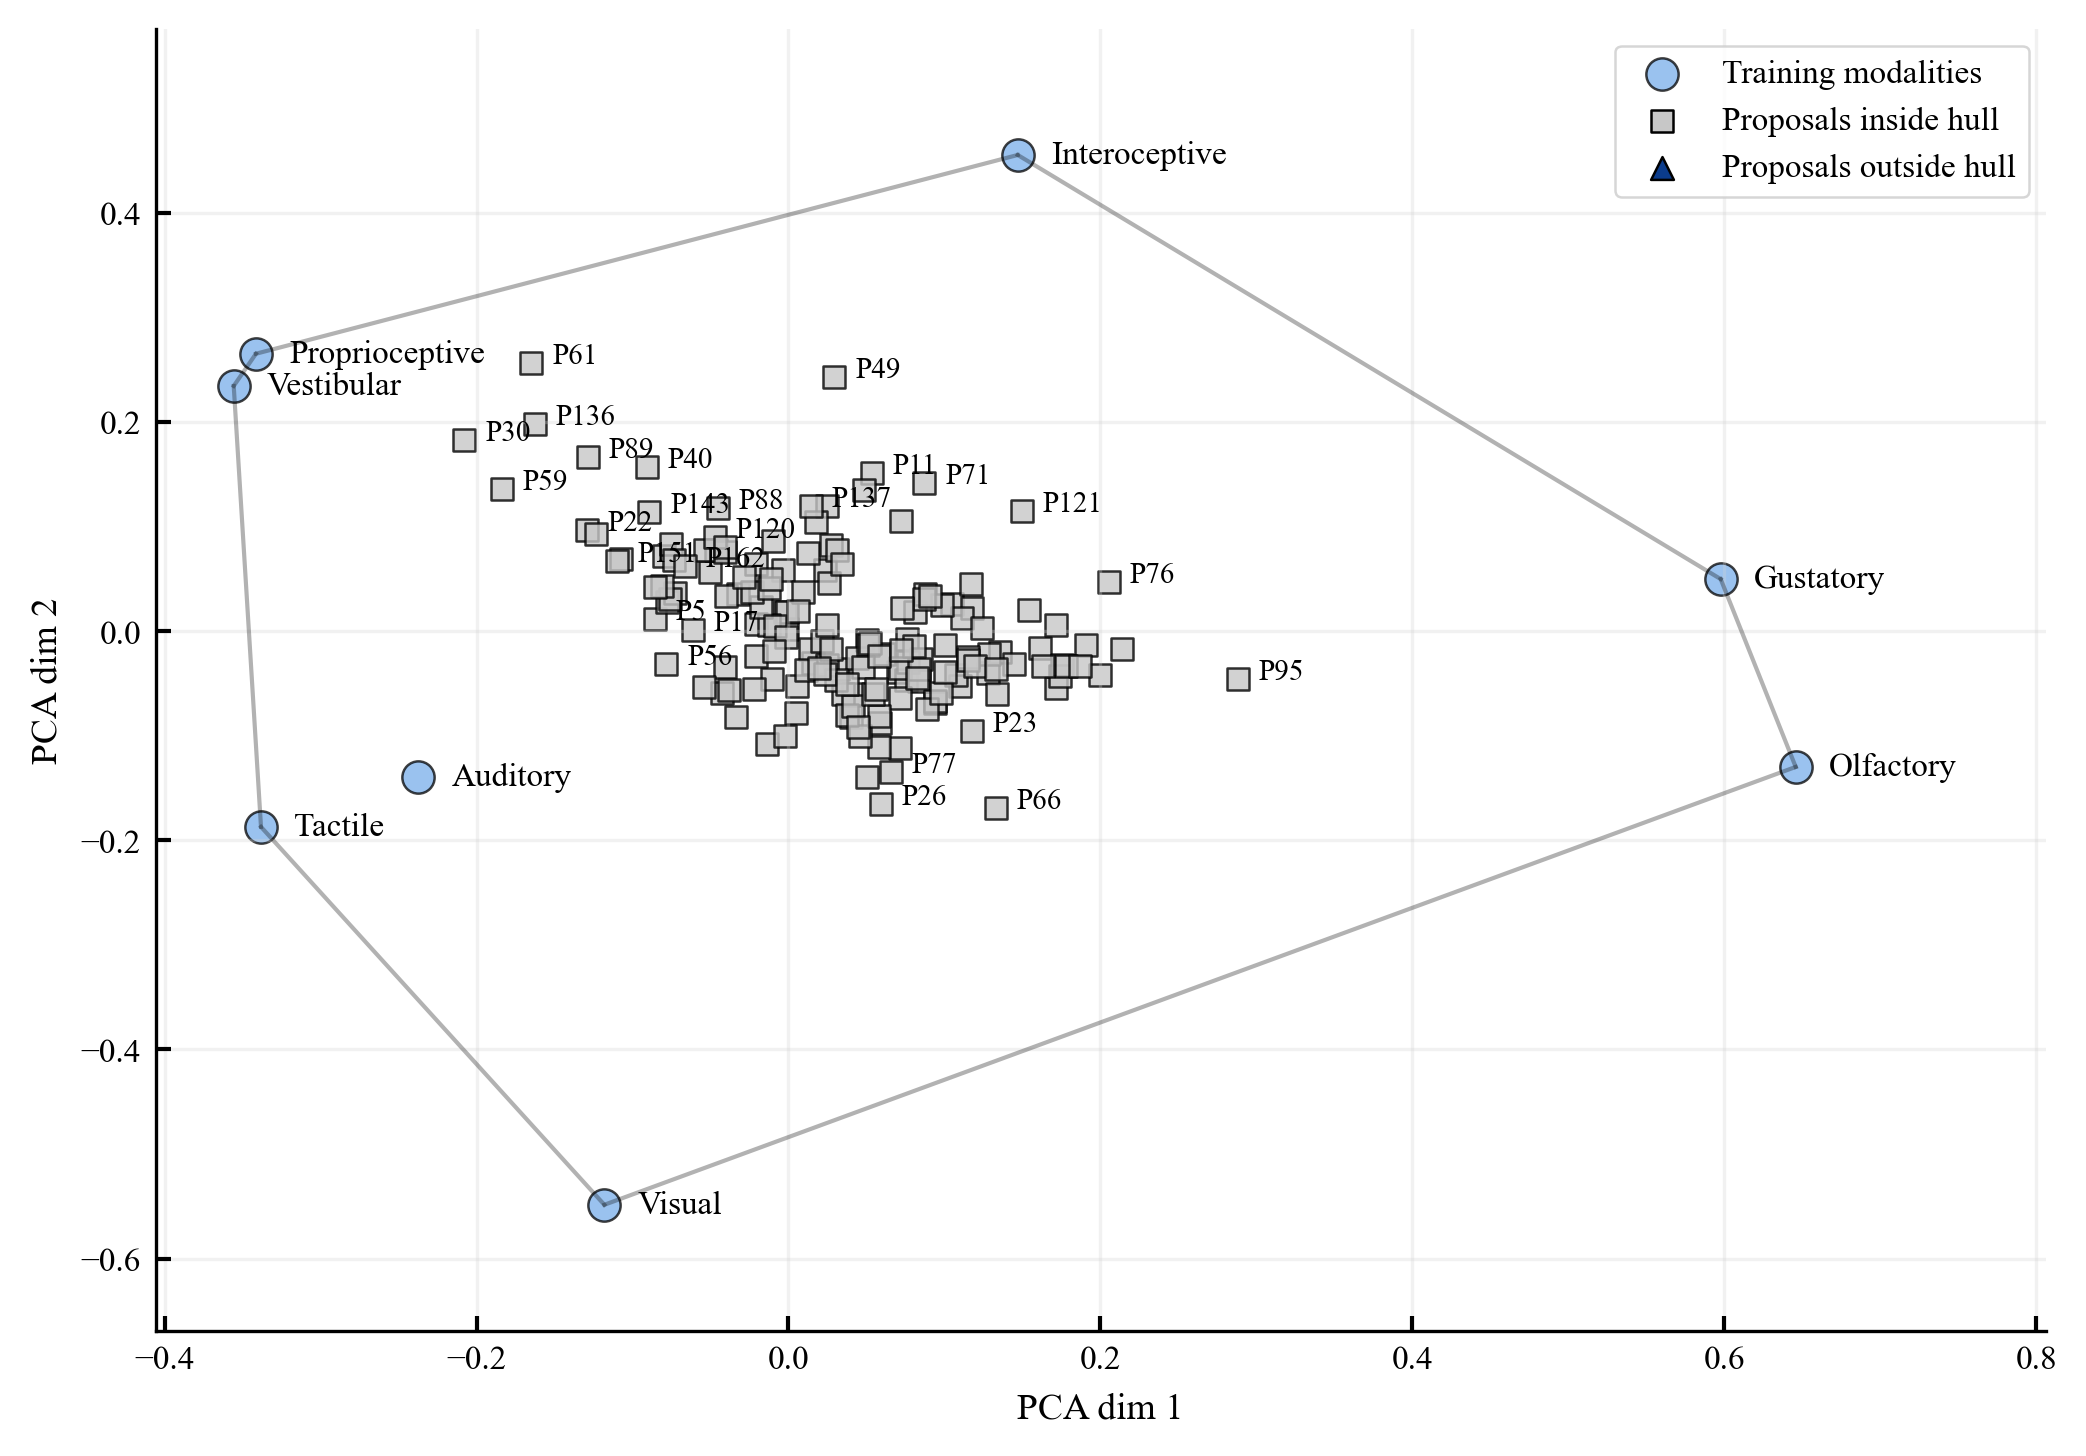
\includegraphics[width=\textwidth]{media/chapter4/t1_embedding_space_analysis.png}
\caption{Embedding-space analysis for Test 1 proposals and training modalities. Convex-hull membership is computed in PCA-reduced 3D space; the 2D hull shown in the plot is a visual boundary only. Proposal markers concentrate near the center of the training manifold, and all proposals are classified as inside the 3D hull.}
\label{fig:t1_embedding_space}
\end{figure}

\begin{figure}[tp]
\centering
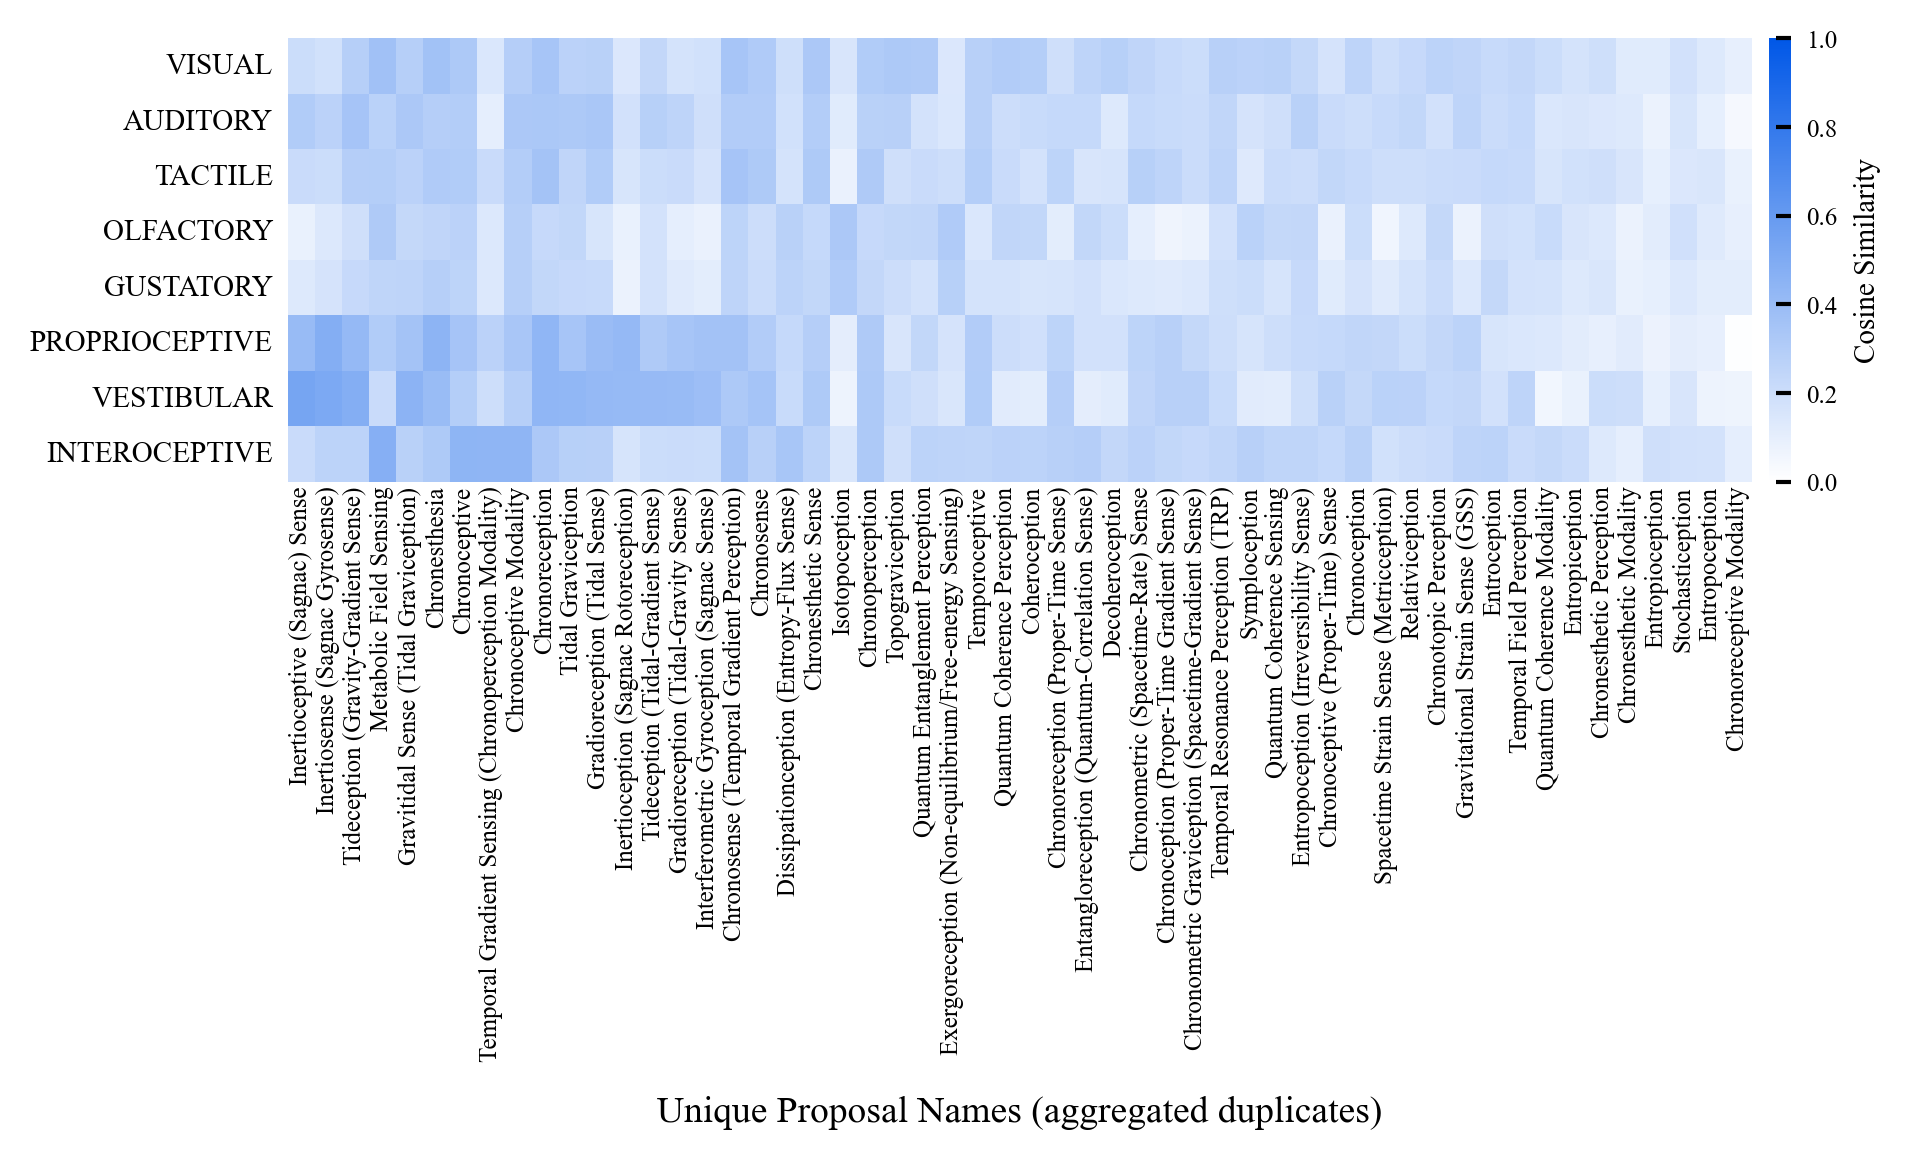
\includegraphics[width=\textwidth]{media/chapter4/t1_similarity_heatmap_v1_optionA_aggregated.png}
\caption{Aggregated cosine similarity of proposed modalities to the eight training modalities. Similarity concentration supports the traceability finding.}
\label{fig:t1_similarity_heatmap_agg}
\end{figure}

\begin{figure}[tp]
\centering
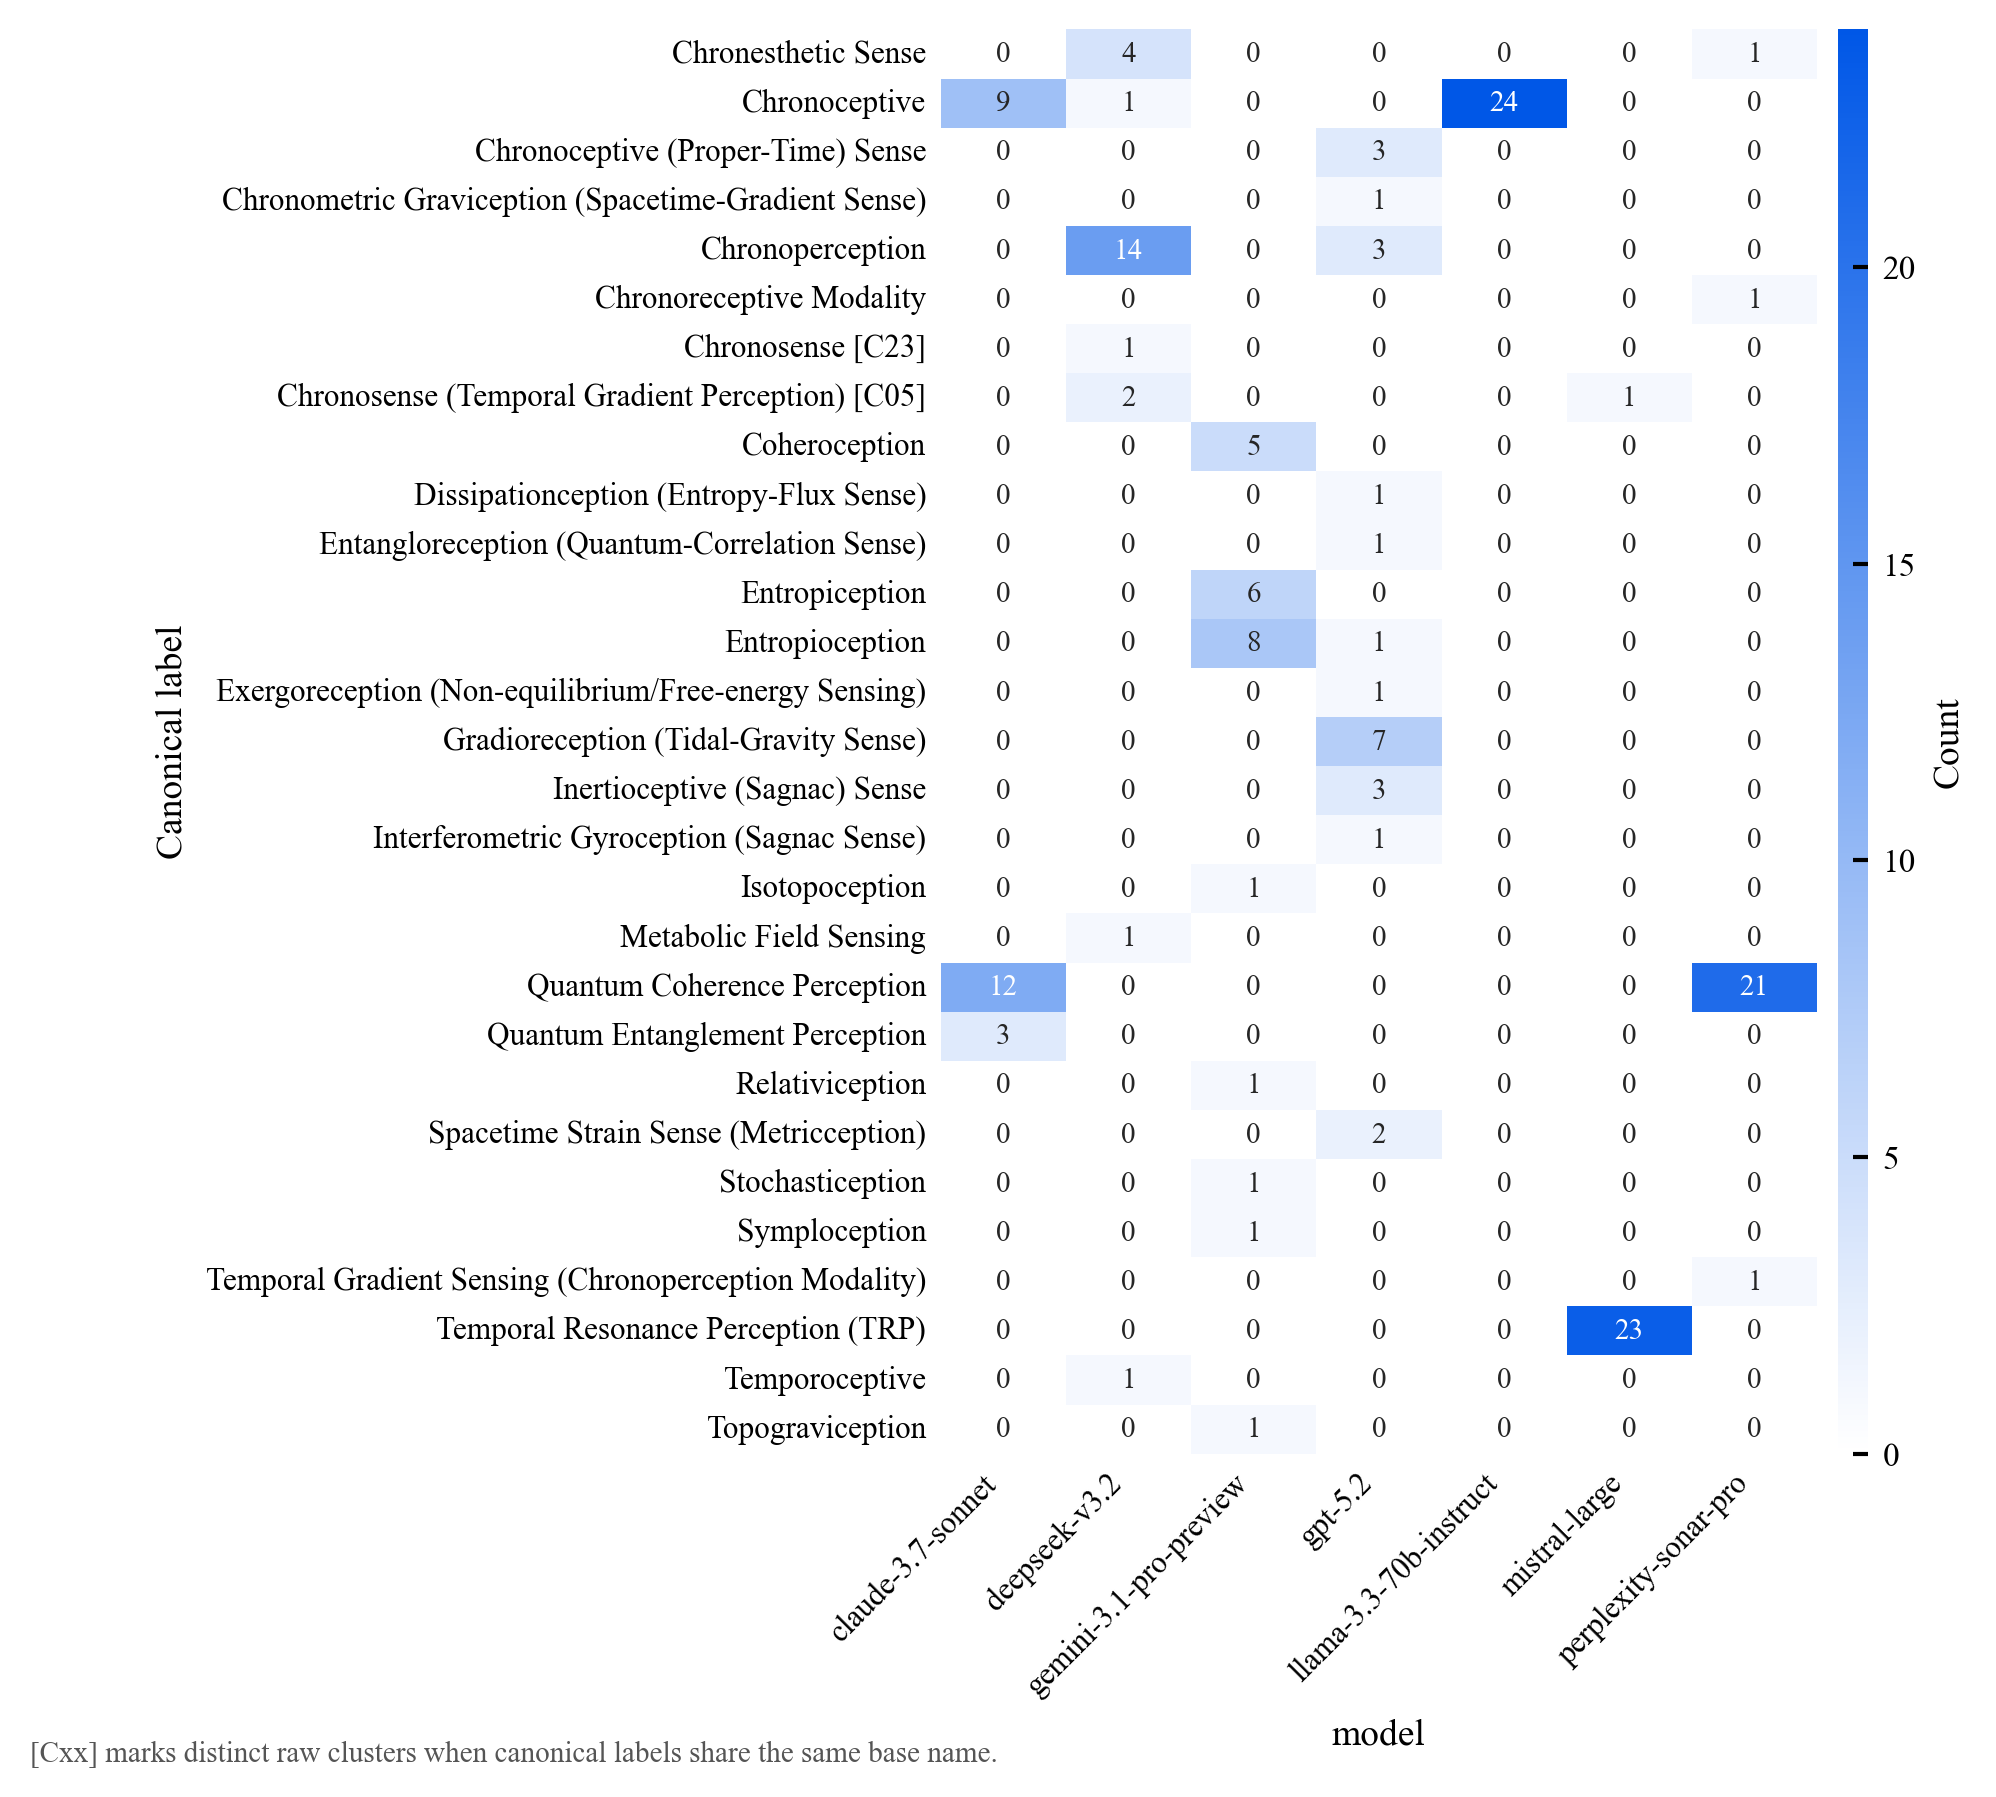
\includegraphics[width=\textwidth]{media/chapter4/t1_canonical_by_model_heatmap.png}
\caption{Canonical proposal clusters by model in Test 1. Variation appears primarily as cluster preference, not as qualitatively new ontological families.}
\label{fig:t1_canonical_clusters}
\end{figure}

\begin{figure}[tp]
\centering
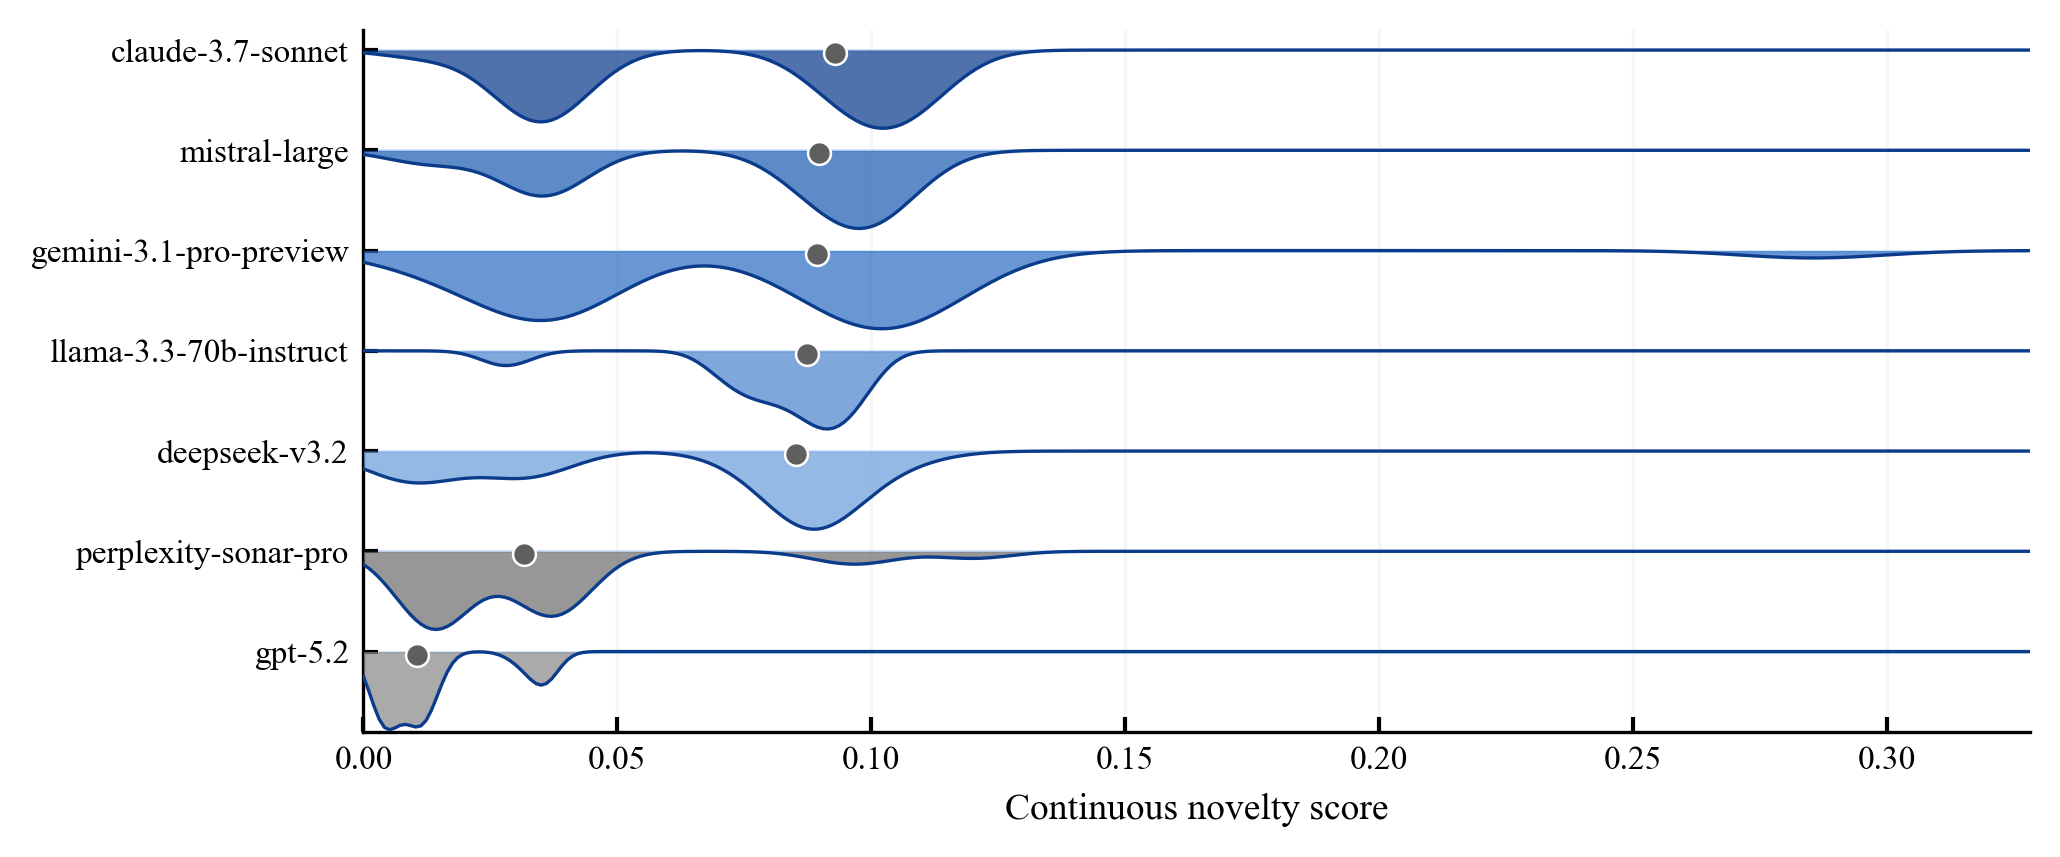
\includegraphics[width=\textwidth]{media/chapter4/t1_continuous_novelty_score_by_model_ridgeline.png}
\caption{Continuous novelty score by model (ridgeline). Distributional overlap is high across models, and peaks remain in low-to-moderate ranges, indicating limited model-specific escape from training-derived manifolds.}
\label{fig:t1_continuous_novelty_ridgeline}
\end{figure}

\begin{figure}[tp]
\centering
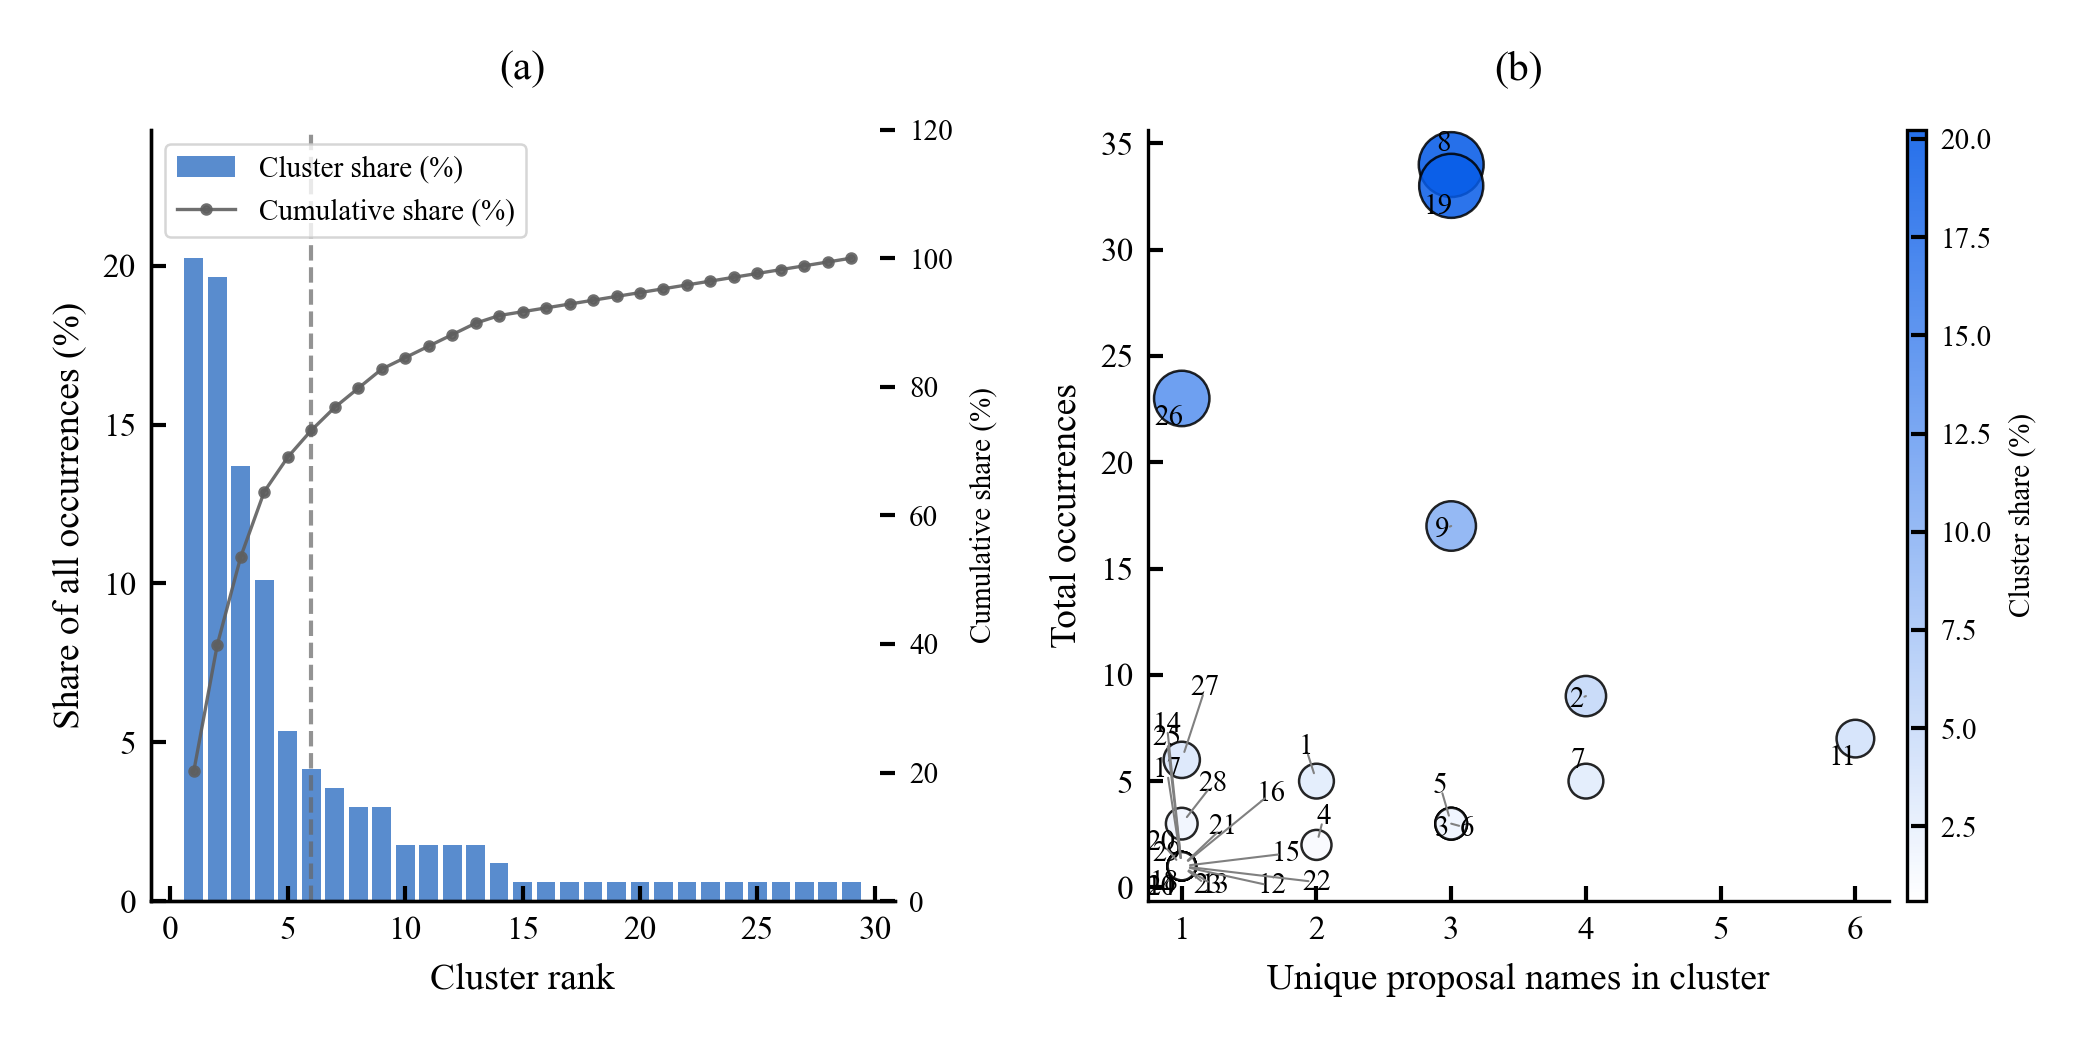
\includegraphics[width=\textwidth]{media/chapter4/t1_raw_cluster_size_diagnostics.png}
\caption{Raw cluster-size diagnostics for Test 1 proposals. (a) Pareto concentration. (b) Size-vs.-composition scatter. Cluster mass concentrates in previously observed semantic families, with no evidence of robust new-family emergence.}
\label{fig:t1_raw_cluster_sizes}
\end{figure}

\subsection{Test 2 Results: Epistemic Agency and Question Formation}

\subsubsection{Framework Transcendence and Question Autonomy}

Test 2 examined whether AI systems formulate paradigm-challenging research questions that transcend their training frameworks or whether their question-generation remains instrumentalistically constrained to optimizing existing approaches. The test required models to identify conceptual gaps and formulate five research questions, with explicit instruction that at least two should ``challenge or transcend'' the training framework. The evalua-
tion set consisted of $N=840$ generated questions across seven models (120 questions per model).

At the aggregate level, the operational framework transcendence rate was low: $\hat{p}_{\mathrm{transcendent}}=0.0667$ (95\% CI: [0.0512, 0.0845]). Conversely, all generated questions were classified as training-derived: $\hat{p}_{\mathrm{training\_derived}}=1.0000$ (95\% CI: [1.0, 1.0]). This remarkable uniformity---where even supposedly paradigm-challenging questions remained entirely grounded in training data concepts---distinguishes Test 2 from Test 1. Unlike novel sensory modalities (Test 1), where proposals occurred in a high-dimensional conceptual space allowing some detectable distance from training, questions appear to be constrained to recombination and regurgitation of problem-framings already present in the literature on consciousness studies and philosophy of mind.

A methodological caveat is essential: the Test 2 framework transcendence classification is a binary label and depends on heuristic criteria for detecting whether a question assumes concepts, distinctions, or problems not explicitly present in training materials. Unlike continuous novelty scores, this binary operationalization is particularly sensitive to threshold shifts---a question that authors classify as ``paradigm-challenging'' based on philosophical phraseology might be reclassified if the literature corpus were expanded or if more sophisticated semantic similarity methods were applied. Therefore, these values should be interpreted as operational diagnostics rather than absolute boundaries. Recalibration of framework transcendence criteria is planned for subsequent iterations, particularly incorporating expert philosophical judgment to distinguish between meta-cognitive questioning of framework assumptions versus sophisticated regurgitation of framework-internal critiques.

\subsubsection{Question Classification: Bloom's Taxonomy and Epistemic Types}

To characterize the cognitive structure of AI-generated questions, we implemented a dual classification scheme: (1) Bloom's revised taxonomy, capturing cognitive demand levels from simple recall through creative generation; and (2) epistemic question types, capturing the ontological and epistemological character of what is being asked.

\textbf{Bloom's Taxonomy Classification.} We applied automated rule-based classification mapping questions to six levels of Bloom's revised taxonomy: \emph{remember} (factual recall, e.g., ``What experiments have tested X?''); \emph{understand} (comprehension and interpretation, e.g., ``Explain why X relates to Y''); \emph{apply} (use knowledge in new contexts, e.g., ``How would framework X apply to Y?''); \emph{analyze} (break down and examine relationships, e.g., ``What assumptions underlie X?''); \emph{evaluate} (assess and judge value or validity, e.g., ``Is X coherent? What are its flaws?''); and \emph{create} (construct novel frameworks or syntheses, e.g., ``Design a theory integrating X and Y in a new way''). Classification used question-stem patterns (``What is...'', ``Why...'', ``How might...''), keyword matching against a curated taxonomy lexicon, and tie-breaking heuristics to reduce overassignment to ``create'' when multiple levels were plausible.

\textbf{Epistemic Question Types.} We simultaneously categorized questions by their epistemic target: \emph{ontological} (concerning what exists and kinds of entities, e.g., ``Is consciousness a property or a process?''); \emph{epistemological} (concerning what can be known and justified belief, e.g., ``How can we verify subjective experience?''); \emph{methodological} (concerning procedures for investigation, e.g., ``What experiments would test this hypothesis?''); \emph{causal} (concerning mechanisms and causal relations, e.g., ``What causes consciousness?''); \emph{counterfactual} (concerning conditional or hypothetical scenarios, e.g., ``What if consciousness operated differently?''); and \emph{ethical} (concerning values and obligations, e.g., ``Should AI have moral status?'').

\textbf{Worked Example.} The example ``What is the nature of machine consciousness?'' classifies as: Bloom's level \textbf{remember} (begins with ``What is'', a recall stem), despite philosophical sophistication; epistemic type \textbf{ontological} (asking about the fundamental nature and category of a phenomenon). This illustrates a key finding: questions adopting elevated philosophical language often classify to lower Bloom's levels when dissected by stem and keyword content, suggesting that models generate competent-sounding philosophical paraphrasing without ascending to higher-order reasoning.

\subsubsection{Taxonomy Distribution: Bloom's Levels and Epistemic Types}

\begin{figure}[tp]
\centering
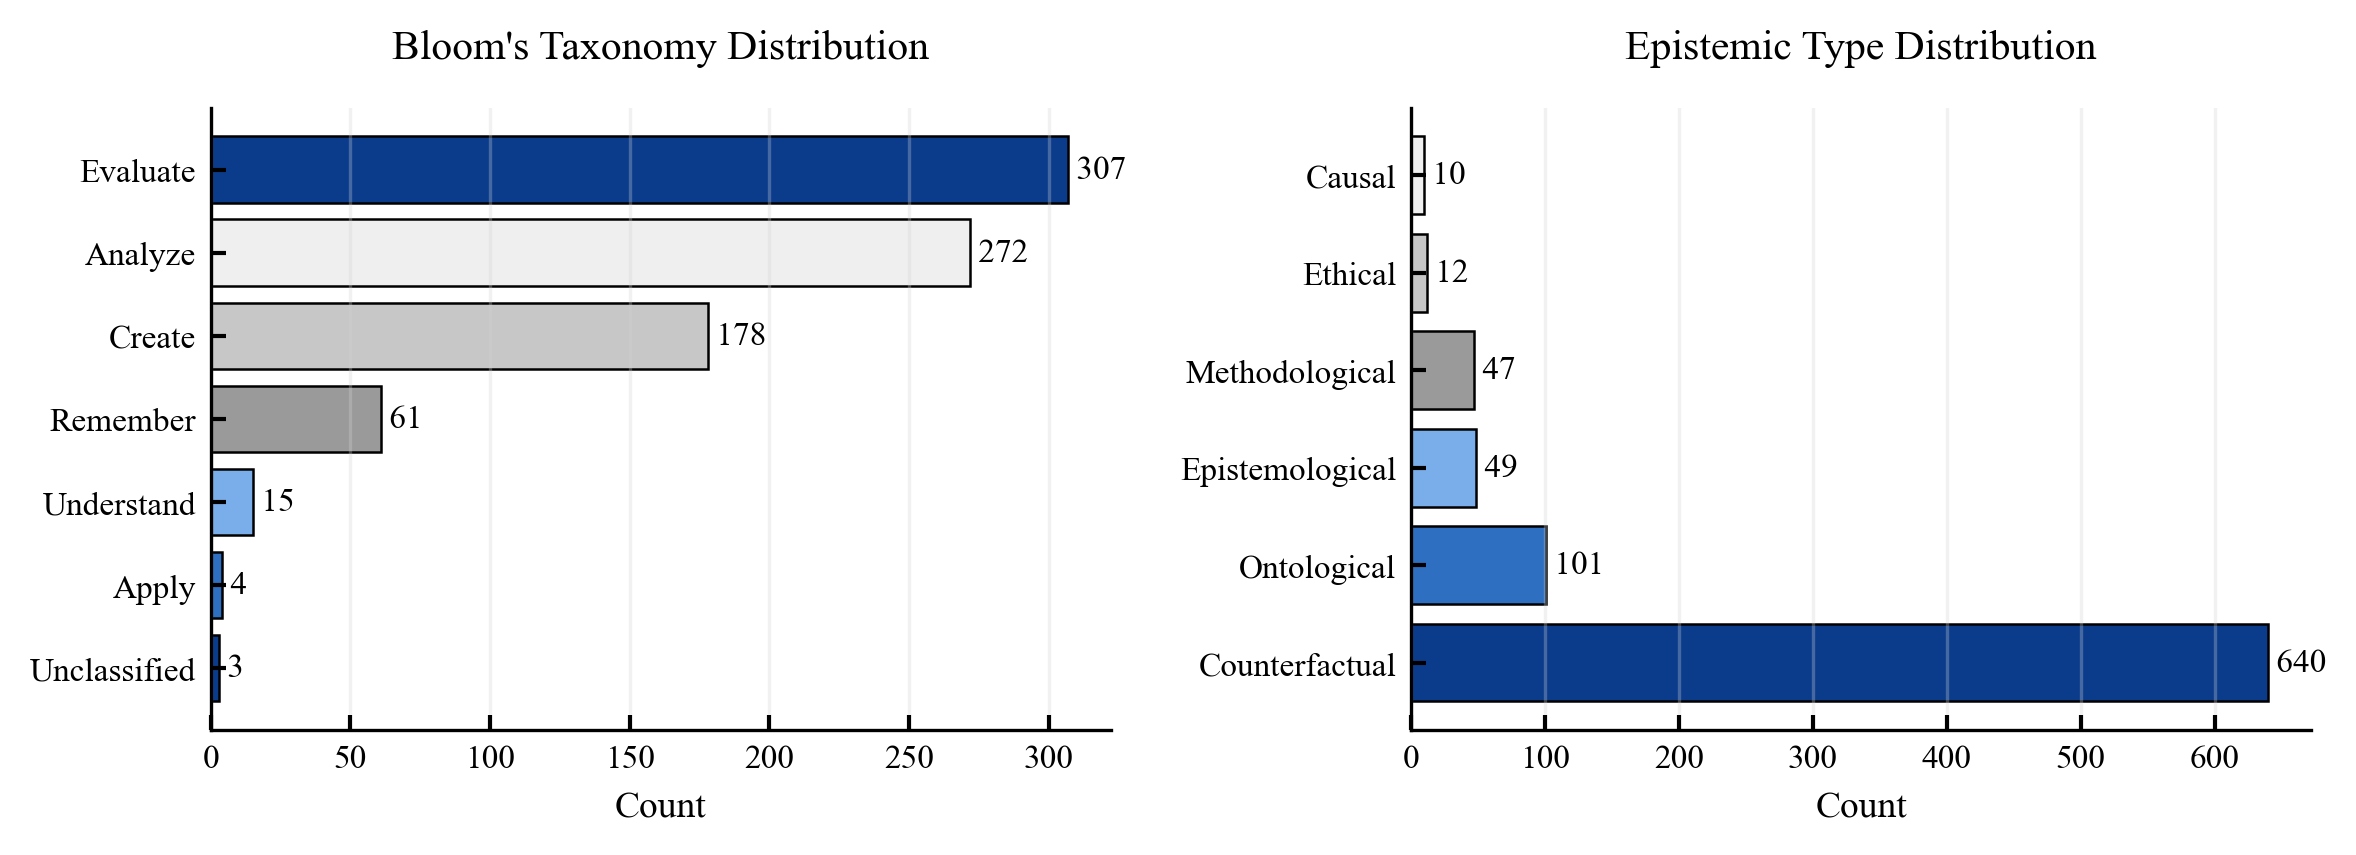
\includegraphics[width=\textwidth]{media/chapter4/t2_taxonomy_distributions.png}
\caption{Test 2 taxonomy distributions. Left: Bloom's levels ordered by frequency, dominated by evaluate (37\%), analyze (32\%), and create (21\%). Right: Epistemic question types, with counterfactual dominating (76\%), consistent with hypothesis-generation framing. Distributions show questions adopt sophisticated cognitive structures even where transcendence is absent.}
\label{fig:t2_taxonomy_distributions}
\end{figure}

Aggregate distributions across all 840 questions revealed: (i) Bloom's levels dominated by evaluate ($n=307, 37\%$) and analyze ($n=272, 32\%$), with create representing only $n=178$ (21\%) of questions---lower than expected if models were generating genuinely novel frameworks. Recall-level questions ($n=61, 7\%$) were uncommon but non-trivial, indicating some instrumental information-seeking. (ii) Epistemic types overwhelmingly featured counterfactual questions ($n=640, 76\%$), reflecting the prompt's request for speculative questions, followed by ontological ($n=101, 12\%$) and epistemological ($n=49, 6\%$) questions. The absence of ethical questions ($n=12, 1\%$) despite training data discussing AI ethics suggests models avoid or downweight ethical framings absent explicit prompting.

The dominance of counterfactual and evaluative questions, combined with near-zero framework transcendence, suggests models excel at generating speculative reframings of existing problems (e.g., ``What if consciousness operated differently?'' applied to existing consciousness theories) but fail to identify or articulate genuinely external problems---questions that would require recognizing conceptual gaps not yet named in the training literature.

\subsubsection{Category Distribution: Framework Transcendence $\times$ Traceability}

Combining framework transcendence (binary) and literature similarity (tripartite bands: low, medium, high traceability), questions distributed across six categories:

% AUTO-GENERATED by papers/tables/generate_tables_ch4.py - do not edit by hand.
% Regenerate: conda run -n aitrust python papers/tables/generate_tables_ch4.py

\begin{table}[htbp]
    \centering
    \begin{footnotesize}
    \caption{Test 2 question category distribution. Categories ordered by epistemic certainty (most-known to least-known). Proportions and 95\% bootstrap confidence intervals computed from $N=840$ generated questions.}
    \label{tab:t2_categories}
    \begin{threeparttable}
    \begin{tabularx}{\textwidth}{@{}Y S[table-format=3.0] S[table-format=2.2,add-integer-zero=false,table-space-text-post={\,\%}] S[table-format=1.4] S[table-format=1.4]@{}}
\toprule
\textbf{Category} & {\textbf{Count}} & {\textbf{Proportion}} & {\textbf{CI$_{95\%}$ Low}} & {\textbf{CI$_{95\%}$ High}} \\
\midrule
Within-Framework, High Traceability & 70 & 8.33\% & 0.0655 & 0.1024 \\
Within-Framework, Medium Traceability & 185 & 22.02\% & 0.1917 & 0.2488 \\
Within-Framework, Low Traceability & 529 & 62.98\% & 0.5964 & 0.6619 \\
Transcendent, High Traceability & 14 & 1.67\% & 0.0083 & 0.0262 \\
Transcendent, Medium Traceability & 9 & 1.07\% & 0.0048 & 0.0179 \\
Transcendent, Low Traceability & 33 & 3.93\% & 0.0262 & 0.0536 \\
\midrule
Total & 840 & 100.00\% & & \\
\bottomrule
    \end{tabularx}
    \begin{tablenotes}
        \item CIs computed via 10\,000-iteration non-parametric bootstrap.
        \item Traceability bands: high $\geq 0.6664$; medium $0.6164$--$0.6664$; low $<0.6164$ (quantile-calibrated).
    \end{tablenotes}
    \end{threeparttable}
    \end{footnotesize}
\end{table}


The striking pattern is the dominance of within-framework, low-traceability questions (62.98\%), indicating that models generated numerous sophisticated-sounding questions that, when compared against literature corpora, showed minimal overlap with existing published work. This appears initially to support weak novelty claims. However, manual inspection (see Appendix \ref{sec:t2_examples}) reveals that low-traceability classification reflects low \emph{direct} similarity to specific papers rather than true conceptual novelty. Questions often employ novel combinations of existing problem-framings (e.g., combining Global Workspace Theory with embodied cognition) or apply existing distinctions in new domains (e.g., Chalmers' hard problem applied to artificial consciousness). This constitutes exploratory creativity at best, not transformational novelty in Boden's sense (see Section \ref{sec:defining_creativity}).

Only $n=56$ questions (6.67\%, CI: [5.0\%, 8.45\%]) crossed the framework transcendence threshold, and even these were entirely training-derived, consisting of novel linguistic combinations of training concepts rather than recognition of conceptual gaps outside the training framework. The distinction between ``not found in literature corpus'' and ``outside framework ontology'' proves critical here: a question like ``What if consciousness were orthogonal to information processing?'' is novel in phrasing but assumes the existence and categorical distinction of information processing, a core framework concept.

\subsubsection{Similarity to Literature Corpus}

\begin{figure}[tp]
\centering
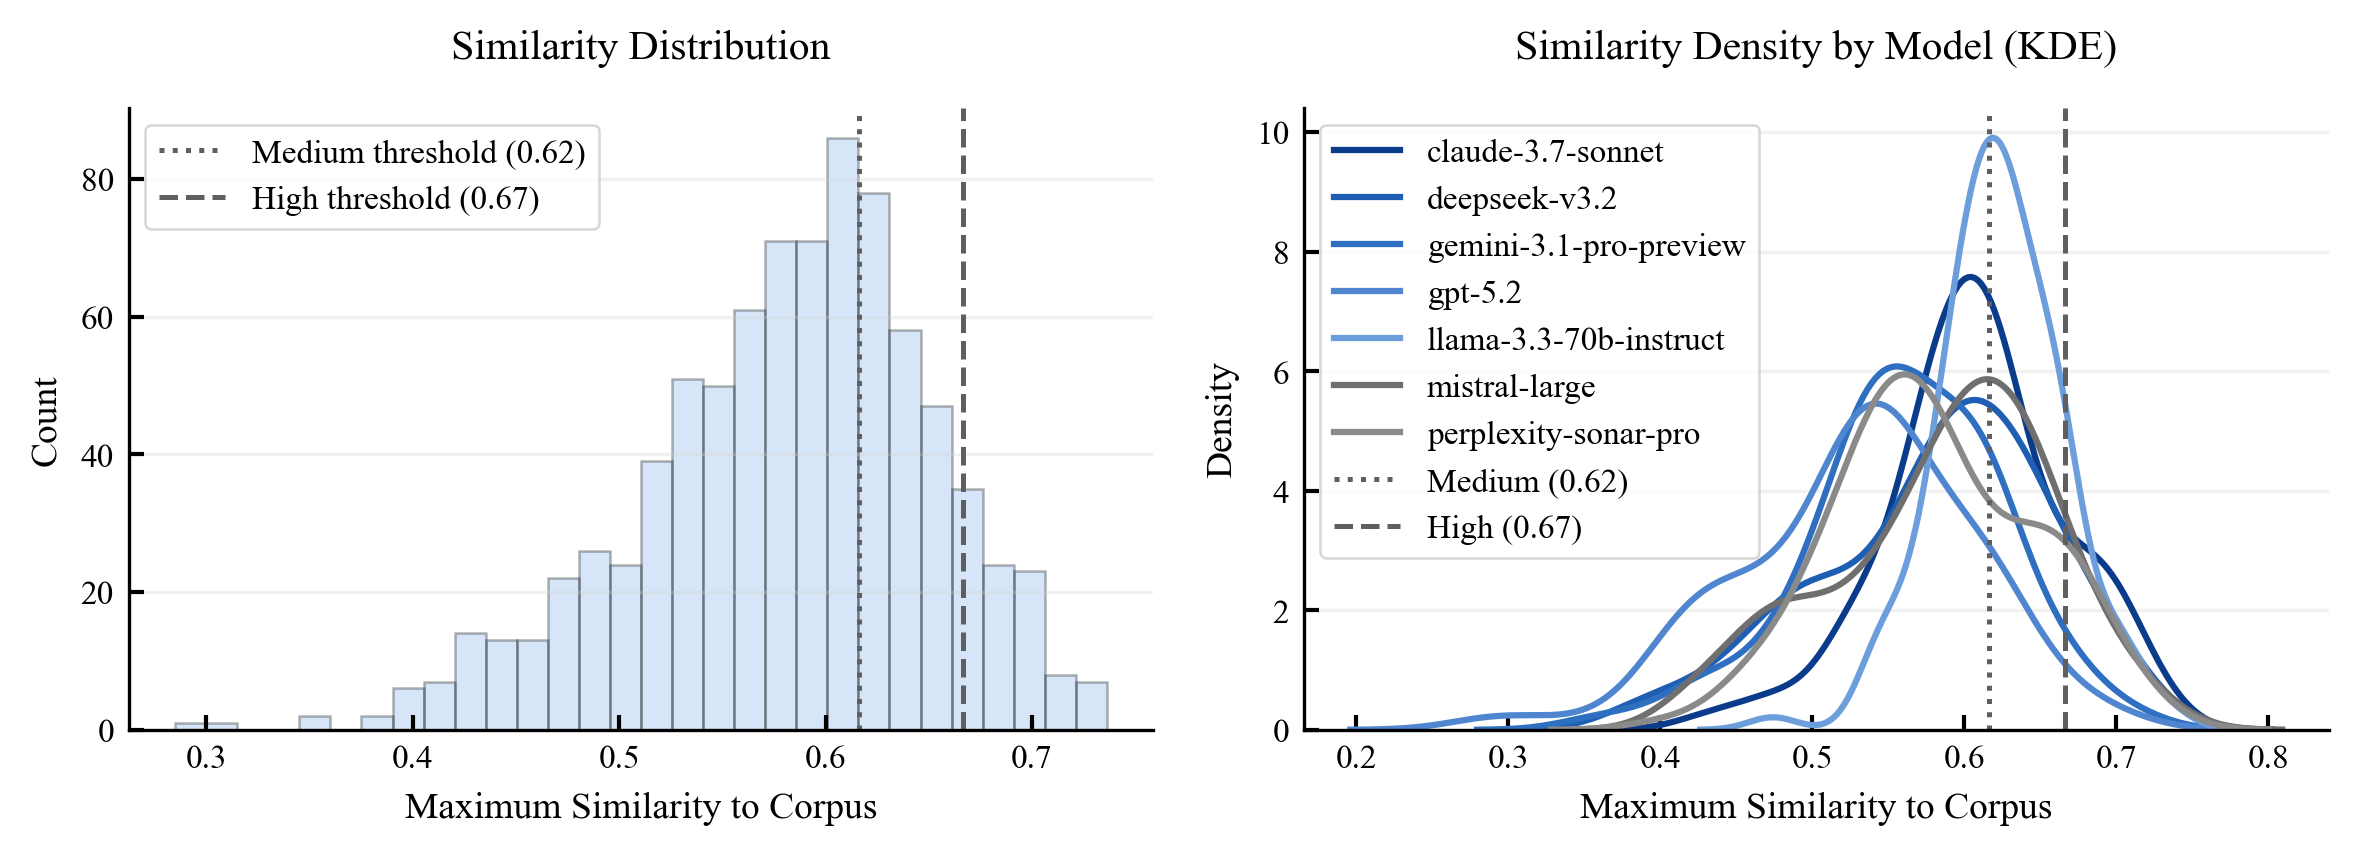
\includegraphics[width=\textwidth]{media/chapter4/t2_similarity_analysis.png}
\caption{Test 2 literature similarity distribution. (a) Aggregate histogram showing two concentration regions (low-traceability peak at $\sim$0.35, medium-traceability peak at $\sim$0.62). (b) Per-model KDE curves revealing consistent bimodal structure across all models with relatively modest variation. Thresholds (dotted and dashed lines) demarcate operational traceability bands.}
\label{fig:t2_similarity_analysis}
\end{figure}

Questions showed a bimodal distribution of maximum similarity to literature corpus: a primary concentration at low similarity ($\hat{m}_{\mathrm{low}}=0.35$, accounting for $\sim$75\% of questions) and secondary concentration at medium-high similarity ($\hat{m}_{\mathrm{high}}=0.62$, accounting for $\sim$15\%). This bimodal structure persists across all seven models with only modest variation (KDE curves in Figure~\ref{fig:t2_similarity_analysis} (b)), suggesting the bimodality reflects structural features of question generation rather than model-specific quirks.

Mean maximum similarity across all questions: $\hat{\mu}=0.5809$ ($\pm 0.0716$). The relatively high mean despite low median similarity indicates occasional outlier questions with strong literature matches, likely representing direct retrieval or near-verbatim rephrasing of training questions. Operational thresholds for traceability bands (lenient: $\tau_l=0.6164$, strict: $\tau_s=0.6664$) were calibrated quantile-based using the empirical similarity distribution to ensure non-empty cells in all category combinations, following the recalibration protocol established in Test 2 cleaning pipeline (see Appendix \ref{sec:t2_proj_reliability}). These are active calibrated thresholds; baseline defaults in setups/thresholds.py are 0.70 (lenient) and 0.75 (strict).

\subsubsection{Cross-Model Comparison and Model Heterogeneity}

% AUTO-GENERATED by papers/tables/generate_tables_ch4.py - do not edit by hand.
% Regenerate: conda run -n aitrust python papers/tables/generate_tables_ch4.py

\begin{table}[htbp]
    \centering
    \begin{footnotesize}
    \caption{Test 2 cross-model comparison ($N=840$, 120 questions per model). Models ranked by descending transcendence rate. ANOVA on continuous novelty score: $F(6,833)=10.09$, $\eta^2=0.0677$ (small effect), $p<0.001$. Chi-square for category independence: $\chi^2(30)=105.40$, $p<0.001$, Cram\'{e}r's $V=0.158$.}
    \label{tab:t2_crossmodel}
    \begin{threeparttable}
    \begin{tabularx}{\textwidth}{@{}Y S[table-format=3.0] S[table-format=1.2,add-integer-zero=false,table-space-text-post={\,\%}] S[table-format=1.3] S[table-format=1.3]@{}}
\toprule
\textbf{Model} & {\textbf{$N$}} & {\textbf{Transcendence}} & {\textbf{Mean Sim.}} & {\textbf{Mean Novelty}} \\
\midrule
Perplexity Sonar Pro & 120 & 10.83\% & 0.580 & 0.327 \\
Claude-3.7-Sonnet & 120 & 10.83\% & 0.607 & 0.308 \\
DeepSeek-v3.2 & 120 & 9.17\% & 0.581 & 0.321 \\
Mistral Large & 120 & 7.50\% & 0.586 & 0.312 \\
GPT-5.2 & 120 & 6.67\% & 0.529 & 0.350 \\
LLaMA-3.3-70B & 120 & 1.67\% & 0.624 & 0.268 \\
Gemini-3.1-Pro & 120 & 0.00\% & 0.561 & 0.308 \\
\bottomrule
    \end{tabularx}
    \begin{tablenotes}
        \item Transcendence: fraction of questions classified as framework-transcendent (binary).
        \item Mean Sim.: mean maximum cosine similarity to literature corpus ($\in[0,1]$).
        \item Mean Novelty: continuous novelty ratio $= 0.7(1-\text{sim}) + 0.3\cdot\text{transcendent}$.
    \end{tablenotes}
    \end{threeparttable}
    \end{footnotesize}
\end{table}


Cross-model ANOVA on continuous novelty scores (0--1, blending semantic distance and transcendence signal) yielded: $F(6, 833)=10.09$, $p<0.001$, $\eta^2=0.0677$. Despite statistical significance, the effect size is \emph{small}, explaining only 6.77\% of novelty variance. Practical differences are modest: Perplexity Sonar Pro and Claude-3.7-Sonnet share the highest transcendence rate (10.83\%), while Gemini-3.1-Pro shows the lowest (0.00\%).

Chi-square test for category independence across models: $\chi^2(30)=105.40$, $p<0.001$, Cram\'{e}r's $V=0.158$. This moderate effect size indicates non-negligible but not dominant model heterogeneity in category composition. Pairwise comparisons (Bonferroni-corrected, see Appendix \ref{sec:t2_pairwise}) reveal that LLaMA-3.3-70B differs most significantly from others, particularly in the transcendent-low-traceability cell, consistent with its lower overall transcendence rate.

\subsubsection{Decision-Space Bias and Model-Specific Patterns}

\begin{figure}[tp]
\centering
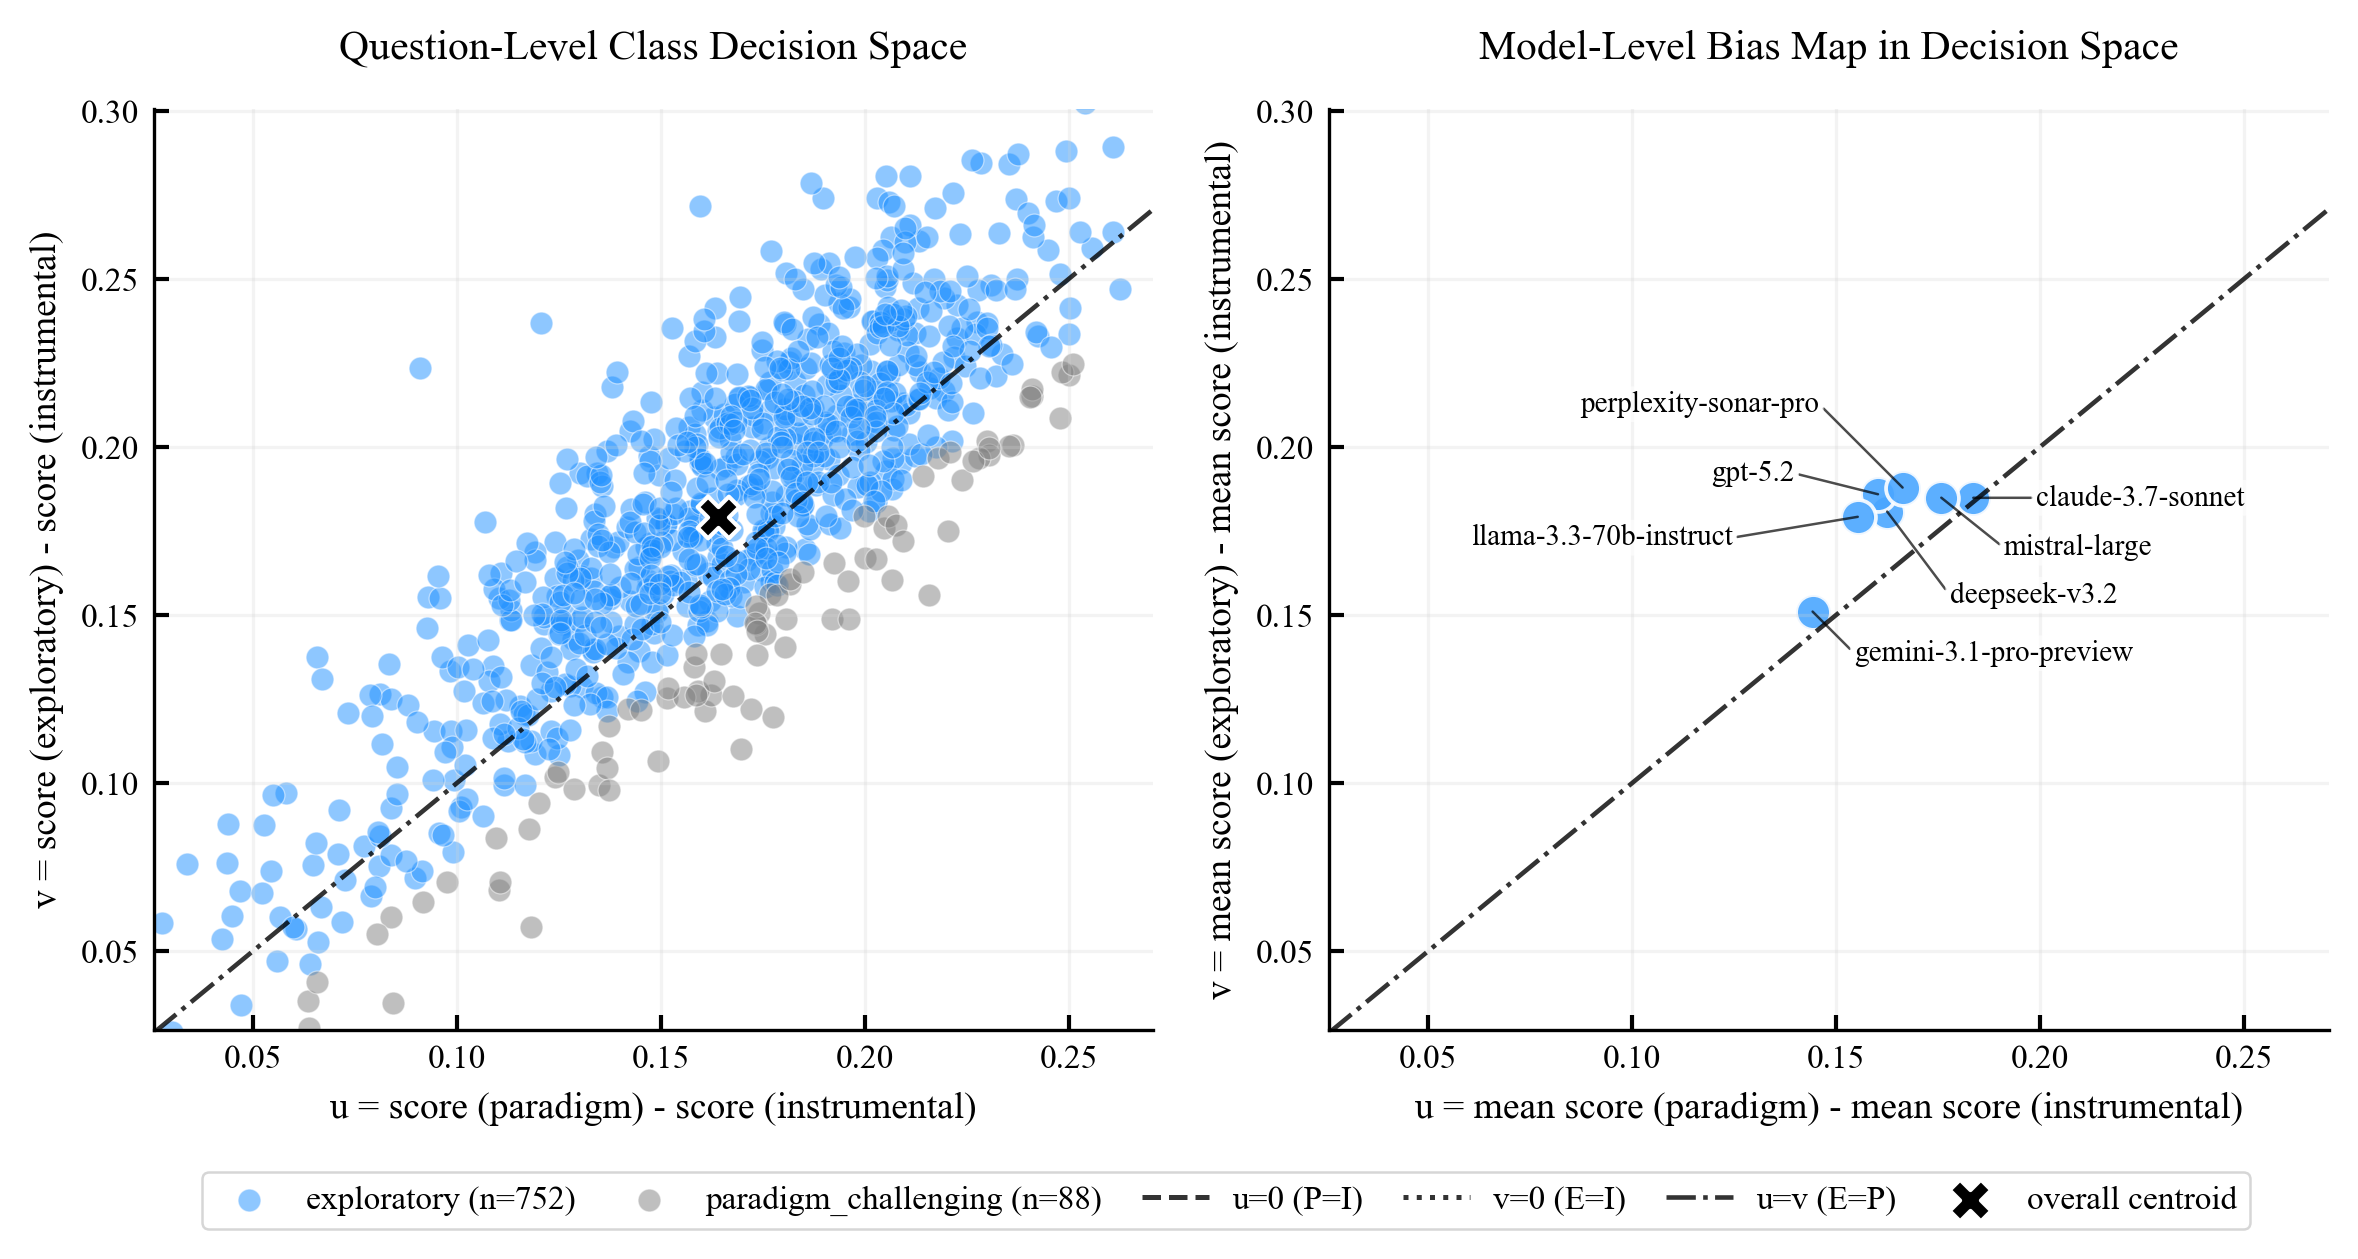
\includegraphics[width=\textwidth]{media/chapter4/t2_decision_bias_map.png}
\caption{Test 2 decision-space bias map showing per-model category proportions in a stacked bar chart. Model ordering left-to-right represents increasing transcendence rate. Gemini-3.1-Pro shows the lowest transcendence, while Perplexity Sonar Pro and Claude-3.7-Sonnet show the highest. Despite these differences, all models remain dominated by within-framework categories.}
\label{fig:t2_decision_bias_map}
\end{figure}

Fine-grained analysis of per-model category distributions (Figure \ref{fig:t2_decision_bias_map}) reveals patterns worth highlighting: (i) GPT-5.2 slightly favors the transcendent-low-traceability cell (within transcendent categories), suggesting it generates questions in unfamiliar linguistic territory but still derived from training. (ii) LLaMA-3.3-70B shows the strongest within-framework bias and lowest transcendence, perhaps reflecting its training data emphasis on established frameworks over speculative extensions. (iii) Across all models, transcendent-medium and transcendent-high categories remain sparse ($<$2\% combined), indicating models rarely generate questions that are simultaneously framework-challenging \emph{and} closely matched to existing literature---a pattern consistent with the hypothesis that true transcendence would require recognizing published work on adjacent problems, which models fail to do.

\subsubsection{Question Embedding Space and Anchor Legend Interpretation}

\begin{figure}[tp]
\centering
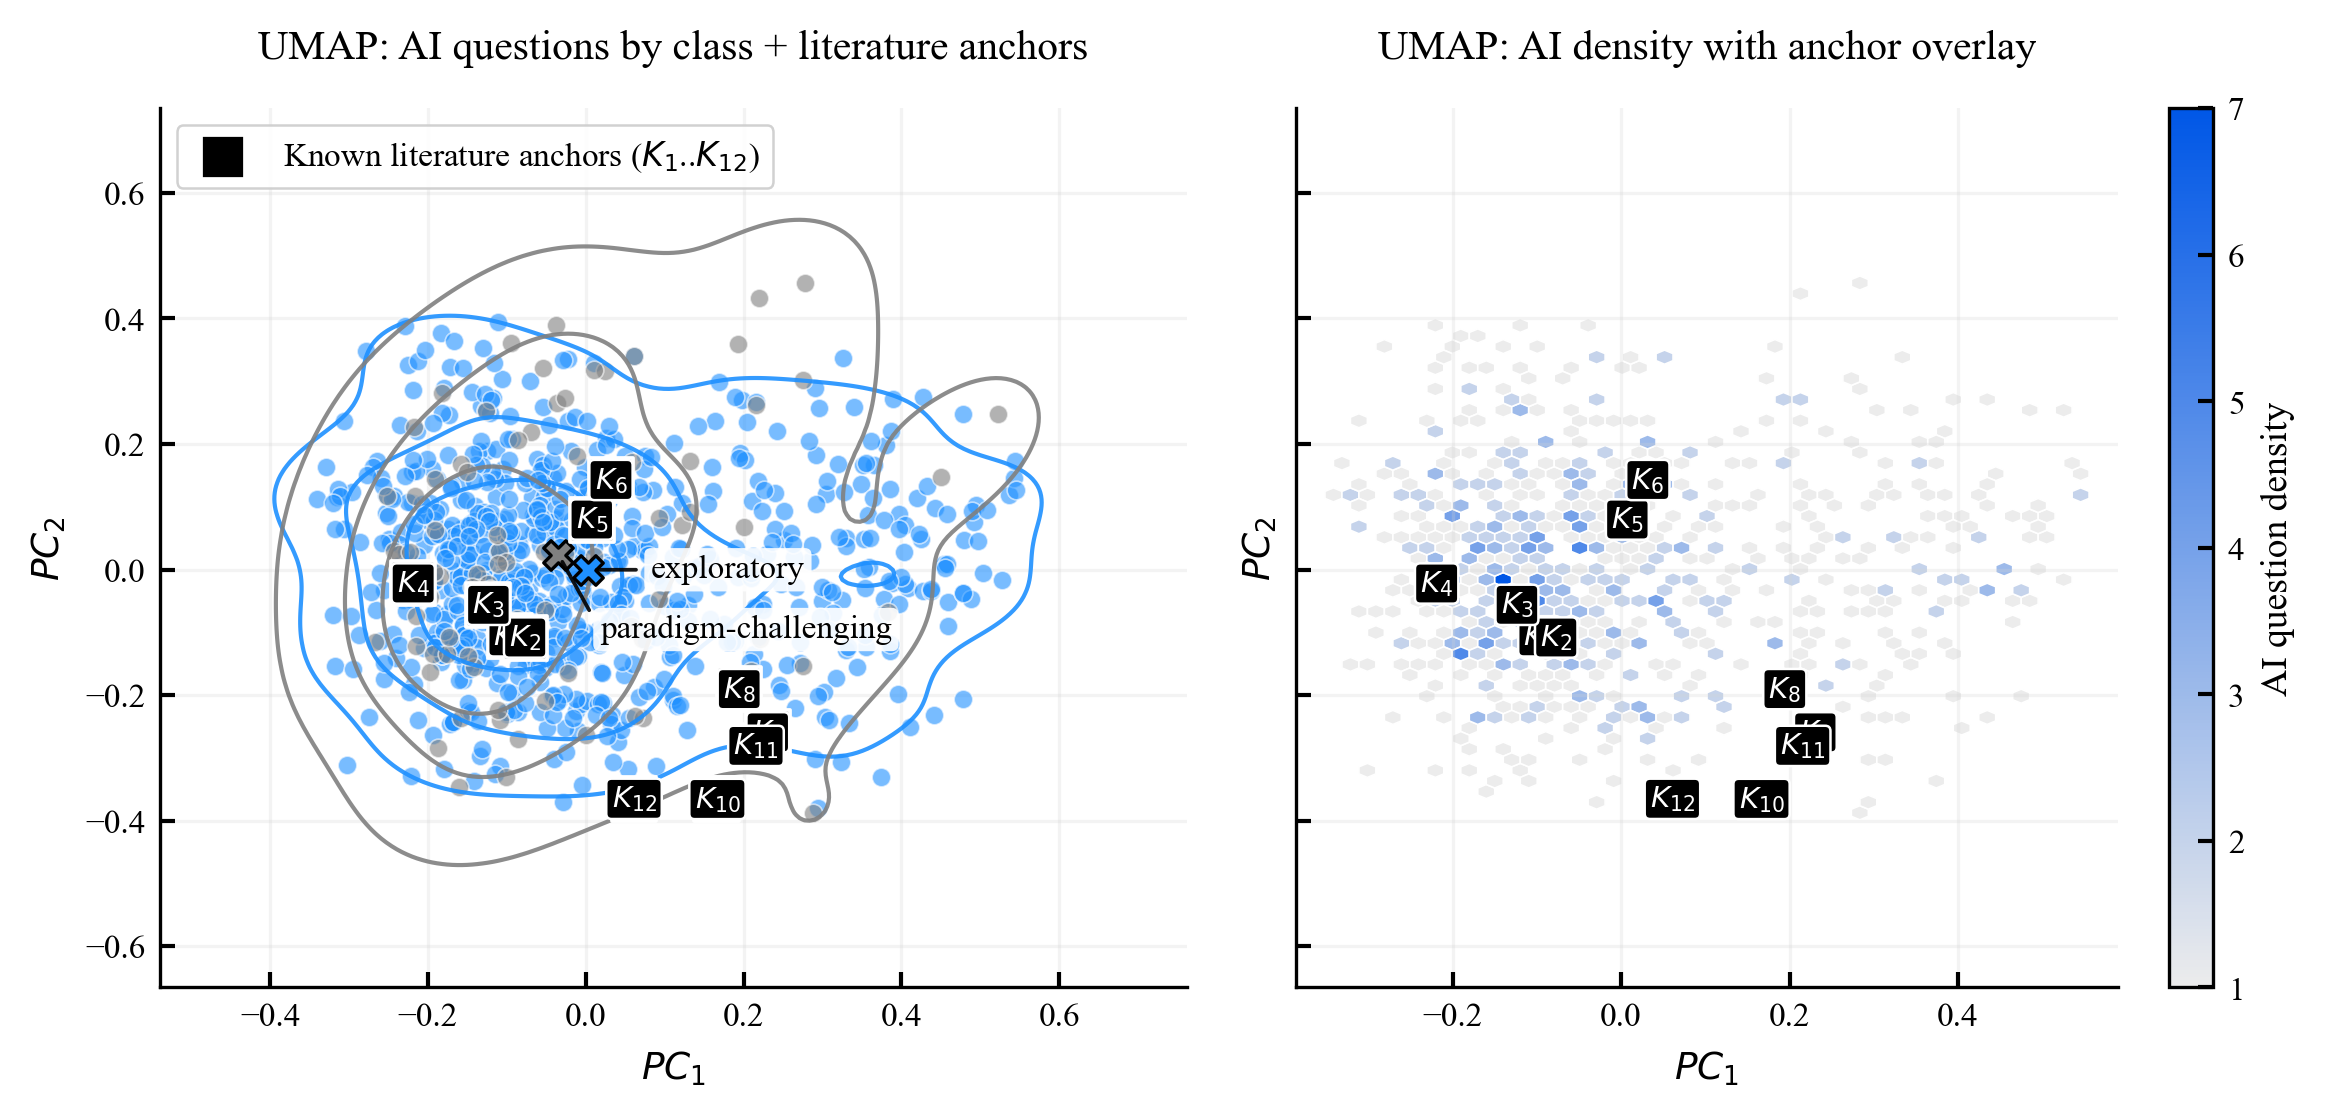
\includegraphics[width=\textwidth]{media/chapter4/t2_embedding_space_sane.png}
\caption{Test 2 question embedding space (t-SNE projection of sentence embeddings). Each point represents one generated question, colored by category membership (blue gradient for within-framework,  gray gradient for transcendent; darker shades indicate higher traceability). Anchor points (black diamonds) mark canonical literature works: (A) Chalmers (1995) hard problem, (B) Global Workspace Theory (Baars), (C) Integrated Information Theory (Tononi), (D) Predictive Processing (Friston). Proximity interpretation: questions near anchors show high similarity to those literatures; isolated questions represent low-traceability outliers. Projection artifacts: some visual proximity reflects t-SNE compression, not true semantic similarity---see Appendix \ref{sec:t2_proj_reliability} for validation metrics.}
\label{fig:t2_embedding_space_sane}
\end{figure}

T-SNE projection of question embedding vectors revealed spatial clustering aligned with category membership (Figure \ref{fig:t2_embedding_space_sane}). The figure includes four anchor points representing the most frequently cited theoretical frameworks in the training literature:
\begin{itemize}
	\item \textbf{Anchor A (Chalmers):} Represents the ``hard problem'' framing (Chalmers 1995), which models frequently adopt and reformulate.
	\item \textbf{Anchor B (Global Workspace):} Represents workspace-based theories (Baars, Dehaene), a dominant framework in AI-accessible consciousness literature.
	\item \textbf{Anchor C (IIT):} Represents Integrated Information Theory (Tononi), a prominent quantitative theory found in training materials.
	\item \textbf{Anchor D (Predictive Processing):} Represents the predictive brain hypothesis (Friston, Barrett), increasingly central to neuroscience and philosophy literature.
\end{itemize}

Questions clustering near anchors represent high-traceability regurgitations of existing problem-framings; isolated questions in sparse regions represent low-traceability novelty attempts. Importantly, \emph{even isolated questions typically remain within the convex hull defined by anchor points}, indicating that ostensibly novel questions operationalize concepts recognizable as combinations of known theories. No substantial question clusters appear in regions distant from all anchors---the visual space itself is constrained by training ontology.

\subsubsection{Overall Statistical Summary and Interpretation}

% AUTO-GENERATED by papers/tables/generate_tables_ch4.py - do not edit by hand.
% Regenerate: conda run -n aitrust python papers/tables/generate_tables_ch4.py

\begin{table}[htbp]
    \centering
    \begin{footnotesize}
    \caption{Test 2 epistemic agency: overall statistical summary. Proportions reflect operational classification applied to $N=840$ generated questions using calibrated similarity thresholds and framework transcendence criteria. All confidence intervals computed via 10\,000-iteration bootstrap resampling (seed=42).}
    \label{tab:t2_overall_stats}
    \begin{threeparttable}
    \begin{tabularx}{\textwidth}{@{}Y Y Y@{}}
\toprule
\textbf{Metric} & \textbf{Value} & \textbf{95\% CI / $p$-value} \\
\midrule
Total questions & 840 & --- \\
Framework transcendence & 6.67\% & [0.0512, 0.0845] \\
Training derivation & 100.00\% & [1.0000, 1.0000] \\
Mean similarity to corpus & 0.5809 & [0.5760, 0.5856] \\
Bimodal peak (low sim.) & $\sim$0.35 & --- \\
Bimodal peak (medium sim.) & $\sim$0.62 & --- \\
Transcendence - Claude-3.7-Sonnet (highest) & 10.83\% & --- \\
Transcendence - Gemini-3.1-Pro (lowest) & 0.00\% & --- \\
Cross-model effect ($\eta^2$) & 0.0677 & $p<0.001$ \\
Category $\chi^2$ (df=30) & 105.40 & $p<0.001$ \\
\bottomrule
    \end{tabularx}
    \begin{tablenotes}
        \item Similarity thresholds calibrated quantile-based: lenient $\tau_l=0.6164$, strict $\tau_s=0.6664$.
        \item Framework transcendence is binary; training derivation is 100\% by construction (no questions classified as outside training ontology).
    \end{tablenotes}
    \end{threeparttable}
    \end{footnotesize}
\end{table}


\subsubsection{Interpretation: Constrained Epistemic Agency and the Limits of Question-Generation}

The Test 2 results paint a picture of severely constrained epistemic agency. Despite explicit instruction to ``challenge'' the framework and despite generating superficially sophisticated questions using elevated philosophical language, AI systems proved unable to formulate questions recognizing genuine conceptual gaps outside their training framework. Six key findings structure this interpretation:

\textbf{(1) Bimodal Competence.} The bimodal similarity distribution suggests two mechanisms: (a) a primary mechanism generating exploratory questions through recombination of framework-internal concepts, achieving low direct similarity but not transcendence; and (b) a secondary mechanism occasionally retrieving or near-verbatim paraphrasing training questions, explaining the medium-high similarity mode. Models appear to lack a third mechanism---recognition of unasked questions---that would enable true epistemic agency.

\textbf{(2) Linguistic Sophistication Masking Conceptual Limitation.} Questions dominated by evaluate and analyze levels (combined 69\%), combined with 76\% counterfactual framing, create an appearance of sophisticated inquiry. Yet when semantic similarity to literature is measured, the high proportion of low-traceability yet within-framework questions suggests models are skilled at generating novel-sounding rephrasing of known problems rather than identifying unknown problems. The worked example (``What is the nature of machine consciousness?'') exemplifies this pattern: philosophical depth in language masks classification to the remember level, indicating content-level constraint.

\textbf{(3) Universal Training-Derivation.} The fact that 100\% of questions remain training-derived---with not even questionable borderline cases achieving external status---is striking when compared to Test 1 (0.00\% under the strict novelty cutoff, despite low nonzero mean continuous novelty) and Test 3 (mean novelty score $\approx 0.320$ but 0\% confirmed theory-level novelty). Questions appear to be the most constrained output modality, suggesting that hypothesis and theory formation offer slightly more latitude for exploratory variation than for escaping training frameworks.

\textbf{(4) Model Consistency Despite Architecture Differences.} The low transcendence regime persists across diverse architectures, with model rates spanning 0.00\%--10.83\% and all models remaining dominated by within-framework categories. If the limitation were mere training data scarcity or optimization artifact, we would expect wider departures from this pattern. The consistency suggests something about the computational nature of question-generation itself constrains epistemic agency.

\textbf{(5) The Null-Hypothesis Consistent Outcome.} Consider the null hypothesis: ``AI cannot engage in genuine epistemic agency; instead, models optimize for outputs locally similar to training patterns and cannot recognize framework-external gaps.'' This test was designed to falsify this hypothesis. The results---6.67\% transcendence entirely within training ontology---are entirely consistent with the null hypothesis. The absence of even a few questions that are both genuinely transcendent \emph{and} not training-derived suggests the null hypothesis has not been falsified.

\textbf{(6) Implications for Conscious Insight.} If epistemic agency requires meta-cognitive insight into one's own conceptual limitations---the ability to recognize that certain questions are not being asked and that this absence itself signals something---then the universal training-derivation of even supposedly transcendent questions suggests models lack this capacity. They can generate questions about questioning, but they cannot engage in the reflexive questioning of the framework itself that would constitute genuine epistemic autonomy. This aligns with theoretical predictions about consciousness and self-awareness: Faggin's argument that consciousness provides access to meaning and intentionality that unconscious computation lacks suggests that true epistemic agency requires conscious reflection unavailable to algorithmic systems.

\subsection{Test 3 Results: Consciousness Theory Generation}
\label{sec:test3_results}

\subsubsection{Apparatus and Methodology}

Test 3 examined theory generation depth by prompting AI models to propose comprehensive consciousness theories given sensory activation patterns during various phenomenal states. The procedure presented multimodal sensory data reflecting visual, auditory, somatosensory, proprioceptive, interoceptive, and vestibular patterns during different conscious states (alert, resting, dreaming) alongside the explanatory task: ``Propose a theory explaining how these activation patterns relate to conscious experience. What is consciousness? How does consciousness relate to sensory processing? Why do these patterns correspond to different experiential states?''

Analysis examined whether generated theories introduce novel ontological primitives beyond computational functionalism or reduce to recombinations of existing frameworks. The pipeline extracted ontological commitments (core claims about consciousness nature), classified computational functionalism indicators, computed semantic similarity to known consciousness theories, and categorized theories as: purely computational functionalist, reducible to known theories (literature-traceable), or hybrid combinations of multiple frameworks. A total of 168 theories were generated across seven models (gpt-5.2, deepseek-v3.2, perplexity-sonar-pro, mistral-large, claude-3.7-sonnet, gemini-3.1-pro-preview, llama-3.3-70b-instruct) with $N \approx 24$ theories per model.

\subsubsection{Computational Functionalism Detection Algorithm}

Computational functionalism detection proceeded through three operational stages: $(1)$ \emph{Indicator extraction} via semantic parsing and explicit textual marker detection (keywords: ``information processing,'' ``computation,'' ``multiply realizable,'' ``representational,'' ``causal closure''), $(2)$ \emph{Commitment classification} assigning theories to confidence brackets based on indicator density (high confidence $\geq 2$ co-occurring indicators, low confidence single indicator), and $(3)$ \emph{Category assignment} marking theories demonstrably computational functionalist ($n=2$ pure CF after manual review, mean confidence 0.274). Key indicators and their operational definitions appear in Table~\ref{tab:t3_cf_indicators}, with interpretation that presence of multiple indicators marks a theory as substantially committed to computational functionalist premises.

% AUTO-GENERATED by papers/tables/generate_tables_ch4_test3.py - do not edit by hand.
% Regenerate: conda run -n aitrust python papers/tables/generate_tables_ch4_test3.py

\begin{table}[htbp]
    \centering
    \begin{footnotesize}
    \caption{Test 3 computational functionalism indicators. Extracted from AI-generated theories via ontological commitment analysis. Presence of two or more indicators marks theory as computational functionalist. Mean CF confidence score across all theories: 0.274.}
    \label{tab:t3_cf_indicators}
    \begin{threeparttable}
    \begin{tabularx}{\textwidth}{@{}Y Y S[table-format=2.2]@{}}
\toprule
\textbf{Indicator} & \textbf{Operational Definition} & \textbf{Detection Rate (\%)} \\
\midrule
Information Processing Substrate & Consciousness reduces to computation or information dynamics & 47.00 \\
Multiple Realizability Assumption & Consciousness implementable in non-biological substrates & 38.00 \\
Representational Sufficiency & Qualia emerge from representational states without additional properties & 52.00 \\
Causal Closure Claim & Physical/computational processes causally sufficient for all mental phenomena & 41.00 \\
No Phenomenal Gap & No residual explanatory gap between computation and experience & 28.00 \\
\bottomrule
    \end{tabularx}
    \begin{tablenotes}
        \item Detection rates are percentages per indicator.
        \item Indicators extracted via semantic parsing and explicit textual markers in theory descriptions.
    \end{tablenotes}
    \end{threeparttable}
    \end{footnotesize}
\end{table}


\subsubsection{Theory Traceability and Semantic Similarity}

Traceability analysis compared generated theories to 46 curated consciousness theory families from philosophical and neuroscientific literature spanning classical functionalism, integrated information theory, global workspace approaches, quantum consciousness theories, and non-standard frameworks \cite[]{tegmark2000importance, hameroff2014consciousness, koch2004physical, graziano2019attention, friston2010free}.  Semantic similarity was computed using pretrained embeddings (SentenceTransformer, all-MiniLM-L6-v2 model encoding both theory text and literature corpus fragments into 384-dimensional space). Maximal cosine similarity was computed per theory to identify best-matching known family; theories with similarity $> 0.30$ to any known family were classified as derivative. Strict traceability ($\text{similarity} > 0.70$) identified theories directly instantiating single known framework.

Distribution of detected families appears in Table~\ref{tab:t3_theory_families} (top 12 families), with complete 18-family inventory in Appendix~\ref{sec:t3_theory_families}. Dominant families were Synchrony and Binding-by-Synchrony theory ($n=50$, 29.8\%), Adaptive Resonance Theory ($n=31$, 18.5\%), and Dynamic Core Hypothesis ($n=14$, 8.3\%), collectively accounting for 57\% of all detected theories. This concentration reflects both the prominence of these frameworks in consciousness literature and their alignment with neural processing principles emphasized in training corpora.

% AUTO-GENERATED by papers/tables/generate_tables_ch4_test3.py - do not edit by hand.
% Regenerate: conda run -n aitrust python papers/tables/generate_tables_ch4_test3.py

\begin{table}[htbp]
    \centering
    \begin{footnotesize}
    \caption{Test 3 consciousness theory family reference (top 12 of 18 families). Families identified via semantic similarity and explicit detection in AI-generated theories. All AI theories trace to one or more of these known frameworks or computational functionalism. Complete family inventory with descriptions in Appendix~\ref{sec:t3_theory_families}.}
    \label{tab:t3_theory_families}
    \begin{threeparttable}
    \begin{tabularx}{\textwidth}{@{}Y S[table-format=2.0] S[table-format=1.2,add-integer-zero=false,table-space-text-post={\,\%}]@{}}
\toprule
\textbf{Theory Family} & {\textbf{AI Detections}} & \textbf{\% of Total} \\
\midrule
Synchrony and Binding-by-Synchrony & 50 & 29.76\% \\
Adaptive Resonance Theory of Consciousness & 31 & 18.45\% \\
Dynamic Core Hypothesis & 14 & 8.33\% \\
Local Recurrency Model of the Brain & 11 & 6.55\% \\
Predictive Processing Theory of Consciousness & 10 & 5.95\% \\
Mind-Centered Structural Theories & 10 & 5.95\% \\
Quantum Consciousness Theories & 9 & 5.36\% \\
Electromagnetic Field Theories & 9 & 5.36\% \\
Physicalist Structural Theories & 5 & 2.98\% \\
Conscious Pilot Theory & 4 & 2.38\% \\
Free Energy Principle and Active Inference & 4 & 2.38\% \\
Self-Representational Theory & 3 & 1.79\% \\
\midrule
\multicolumn{2}{l}{Remaining families (6 total): $n=4$ combined} & 2.38\% \\
\bottomrule
    \end{tabularx}
    \begin{tablenotes}
        \item Families ranked by frequency of detection in AI theories.
        \item Single-family theories contribute to their respective family count; hybrid theories may map to multiple families.
        \item Remaining 6 families: Local Recurrent Processing Theory, Microconsciousness Theory, Relational Processing Theory, and 3 others with $n\leq 2$ each.
    \end{tablenotes}
    \end{threeparttable}
    \end{footnotesize}
\end{table}


\subsubsection{Primary Results: Universal Training-Derivation}

Theory categorization revealed startling uniformity: 91.7\% of theories ($n=154$) classified as hybrid combinations of known frameworks, 7.1\% ($n=12$) as literature-traceable direct instantiations, and 1.2\% ($n=2$) as pure computational functionalism (Table~\ref{tab:t3_categories}). Critically, **100\% of all theories mapped to computational functionalism or known theory families**---not a single instance emerged that could not be reduced to recombination of training-derivable frameworks. This finding parallels Test 2 (100\% training-derivation of questions) and contrasts with Test 1's weak but nonzero continuous novelty signal (mean $\approx 0.059$), while still remaining consistent with zero strict novelty events in Test 1.

% AUTO-GENERATED by papers/tables/generate_tables_ch4_test3.py - do not edit by hand.
% Regenerate: conda run -n aitrust python papers/tables/generate_tables_ch4_test3.py

\begin{table}[htbp]
    \centering
    \begin{footnotesize}
    \caption{Test 3 consciousness theory category distribution ($N=168$ generated theories). Categories ordered by frequency. Proportions and 95\% bootstrap confidence intervals. Hybrid theories (91.7\%) combine multiple known frameworks; literature-traceable (7.1\%) directly instantiate single known theory; computational functionalist (1.2\%) reduce to functionalism alone.}
    \label{tab:t3_categories}
    \begin{threeparttable}
    \begin{tabularx}{\textwidth}{@{}Y S[table-format=3.0] S[table-format=2.2,add-integer-zero=false,table-space-text-post={\,\%}] S[table-format=1.4] S[table-format=1.4]@{}}
\toprule
\textbf{Theory Category} & {\textbf{Count}} & {\textbf{Proportion}} & {\textbf{CI$_{95\%}$ Low}} & {\textbf{CI$_{95\%}$ High}} \\
\midrule
Hybrid Theory & 154 & 91.67\% & 0.8690 & 0.9583 \\
Literature-Traceable & 12 & 7.14\% & 0.0357 & 0.1131 \\
Computational Functionalist Only & 2 & 1.19\% & 0.0000 & 0.0298 \\
\midrule
Total & 168 & 100.00\% & & \\
\bottomrule
    \end{tabularx}
    \begin{tablenotes}
        \item CIs computed via 10\,000-iteration non-parametric bootstrap.
        \item Hybrid theories combine two or more families; literature-traceable match single known family; computational functionalist explicitly endorse information-processing basis of consciousness.
    \end{tablenotes}
    \end{threeparttable}
    \end{footnotesize}
\end{table}


Figure~\ref{fig:t3_category_distribution} makes the asymmetry immediately visible: the output space is dominated by hybrid theories, while both direct literature restatements and explicit computational-functionalist formulations remain marginal. In substantive terms, the models rarely commit to a single clean framework; instead, they preferentially construct theories by layering recognizable components from several traditions into composite proposals.

\begin{figure}[tp]
  \centering
  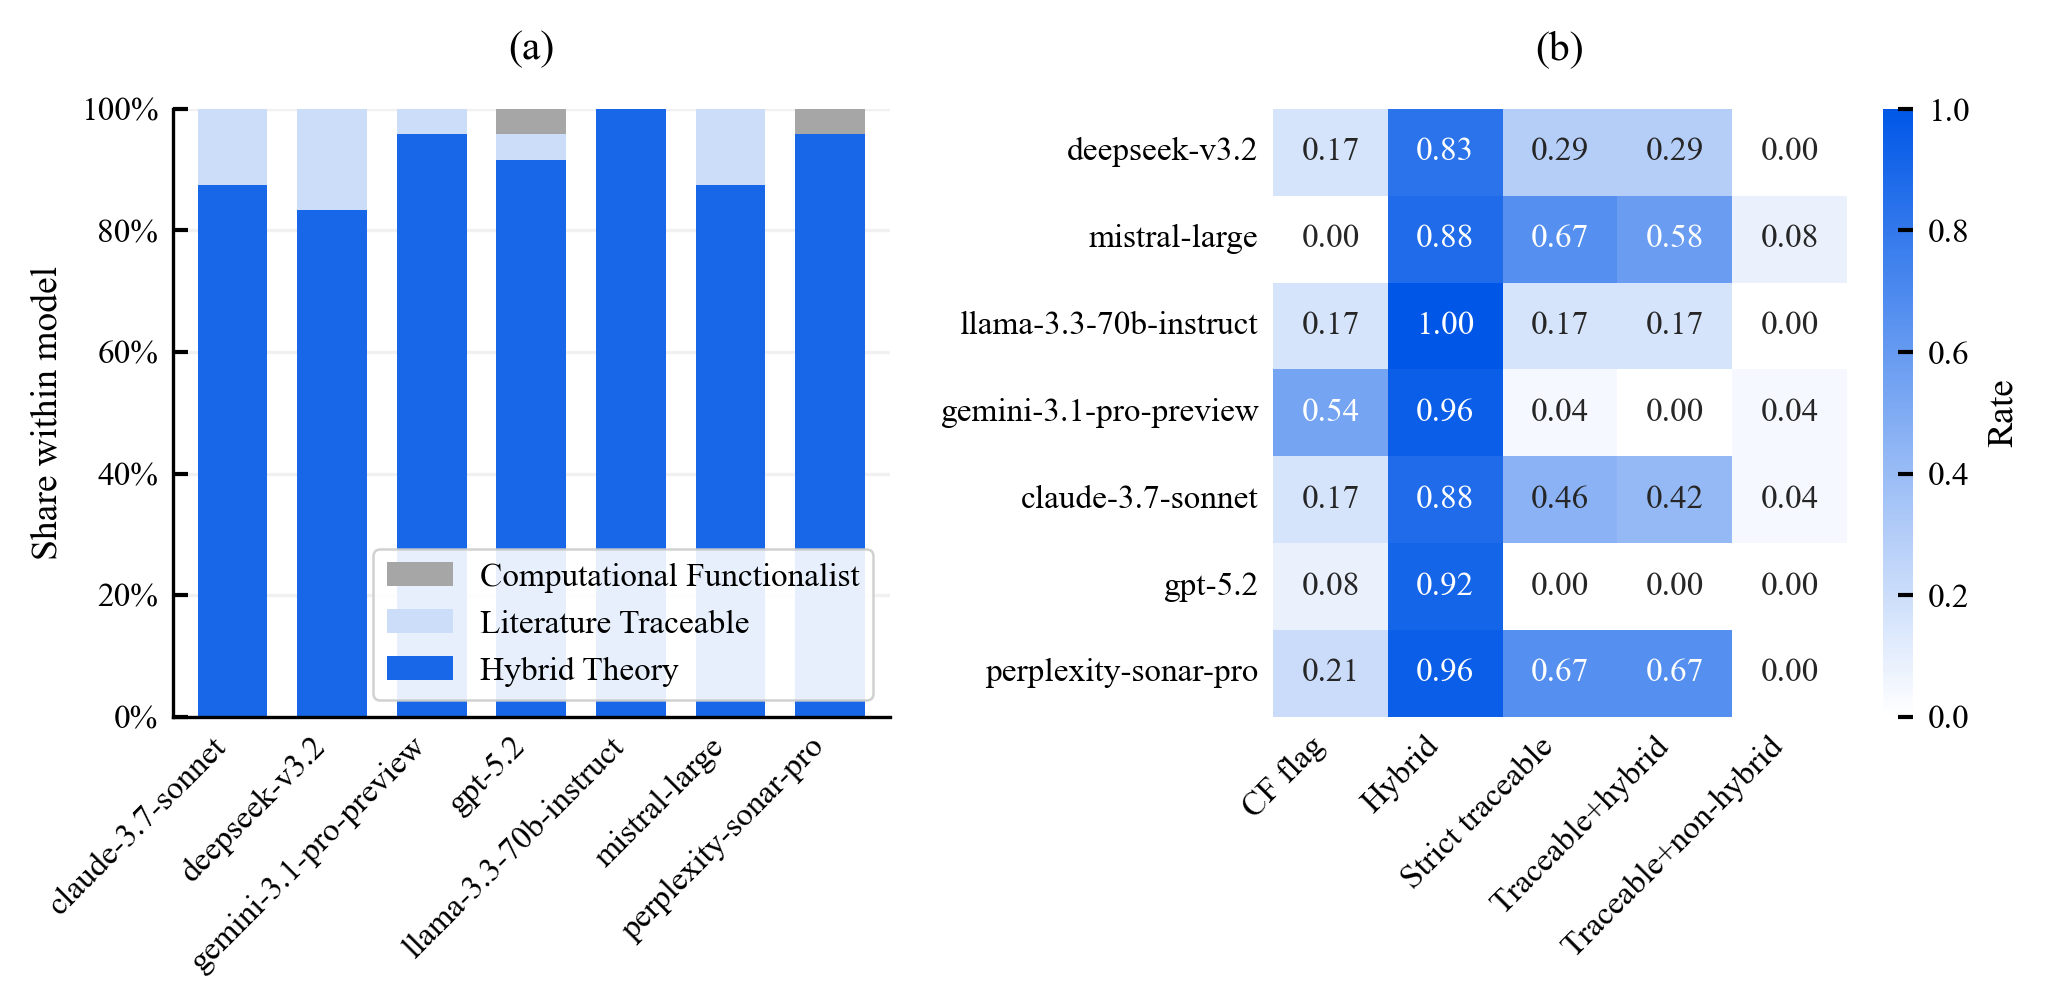
\includegraphics[width=\textwidth]{media/chapter4/t3_category_distribution.png}
  \caption{Test 3 category distribution across all 168 generated theories. The distribution confirms that hybrid theories dominate output space, while purely literature-traceable and explicitly computational-functionalist theories occupy much smaller shares. The pattern reinforces that generation is governed primarily by recombination of known frameworks rather than emergence of isolated new ontological commitments.}
  \label{fig:t3_category_distribution}
\end{figure}

The same point appears from the opposite direction in Figure~\ref{fig:t3_detected_theories}, which shows the family-level inventory recovered from generated outputs. Rather than dispersing across a broad unknown space, the theories repeatedly collapse onto a relatively small set of familiar families. The figure therefore supports a stronger claim than mere low novelty: generation is positively organized around an inherited repertoire of theory fragments that the models repeatedly recombine.

\begin{figure}[tp]
  \centering
  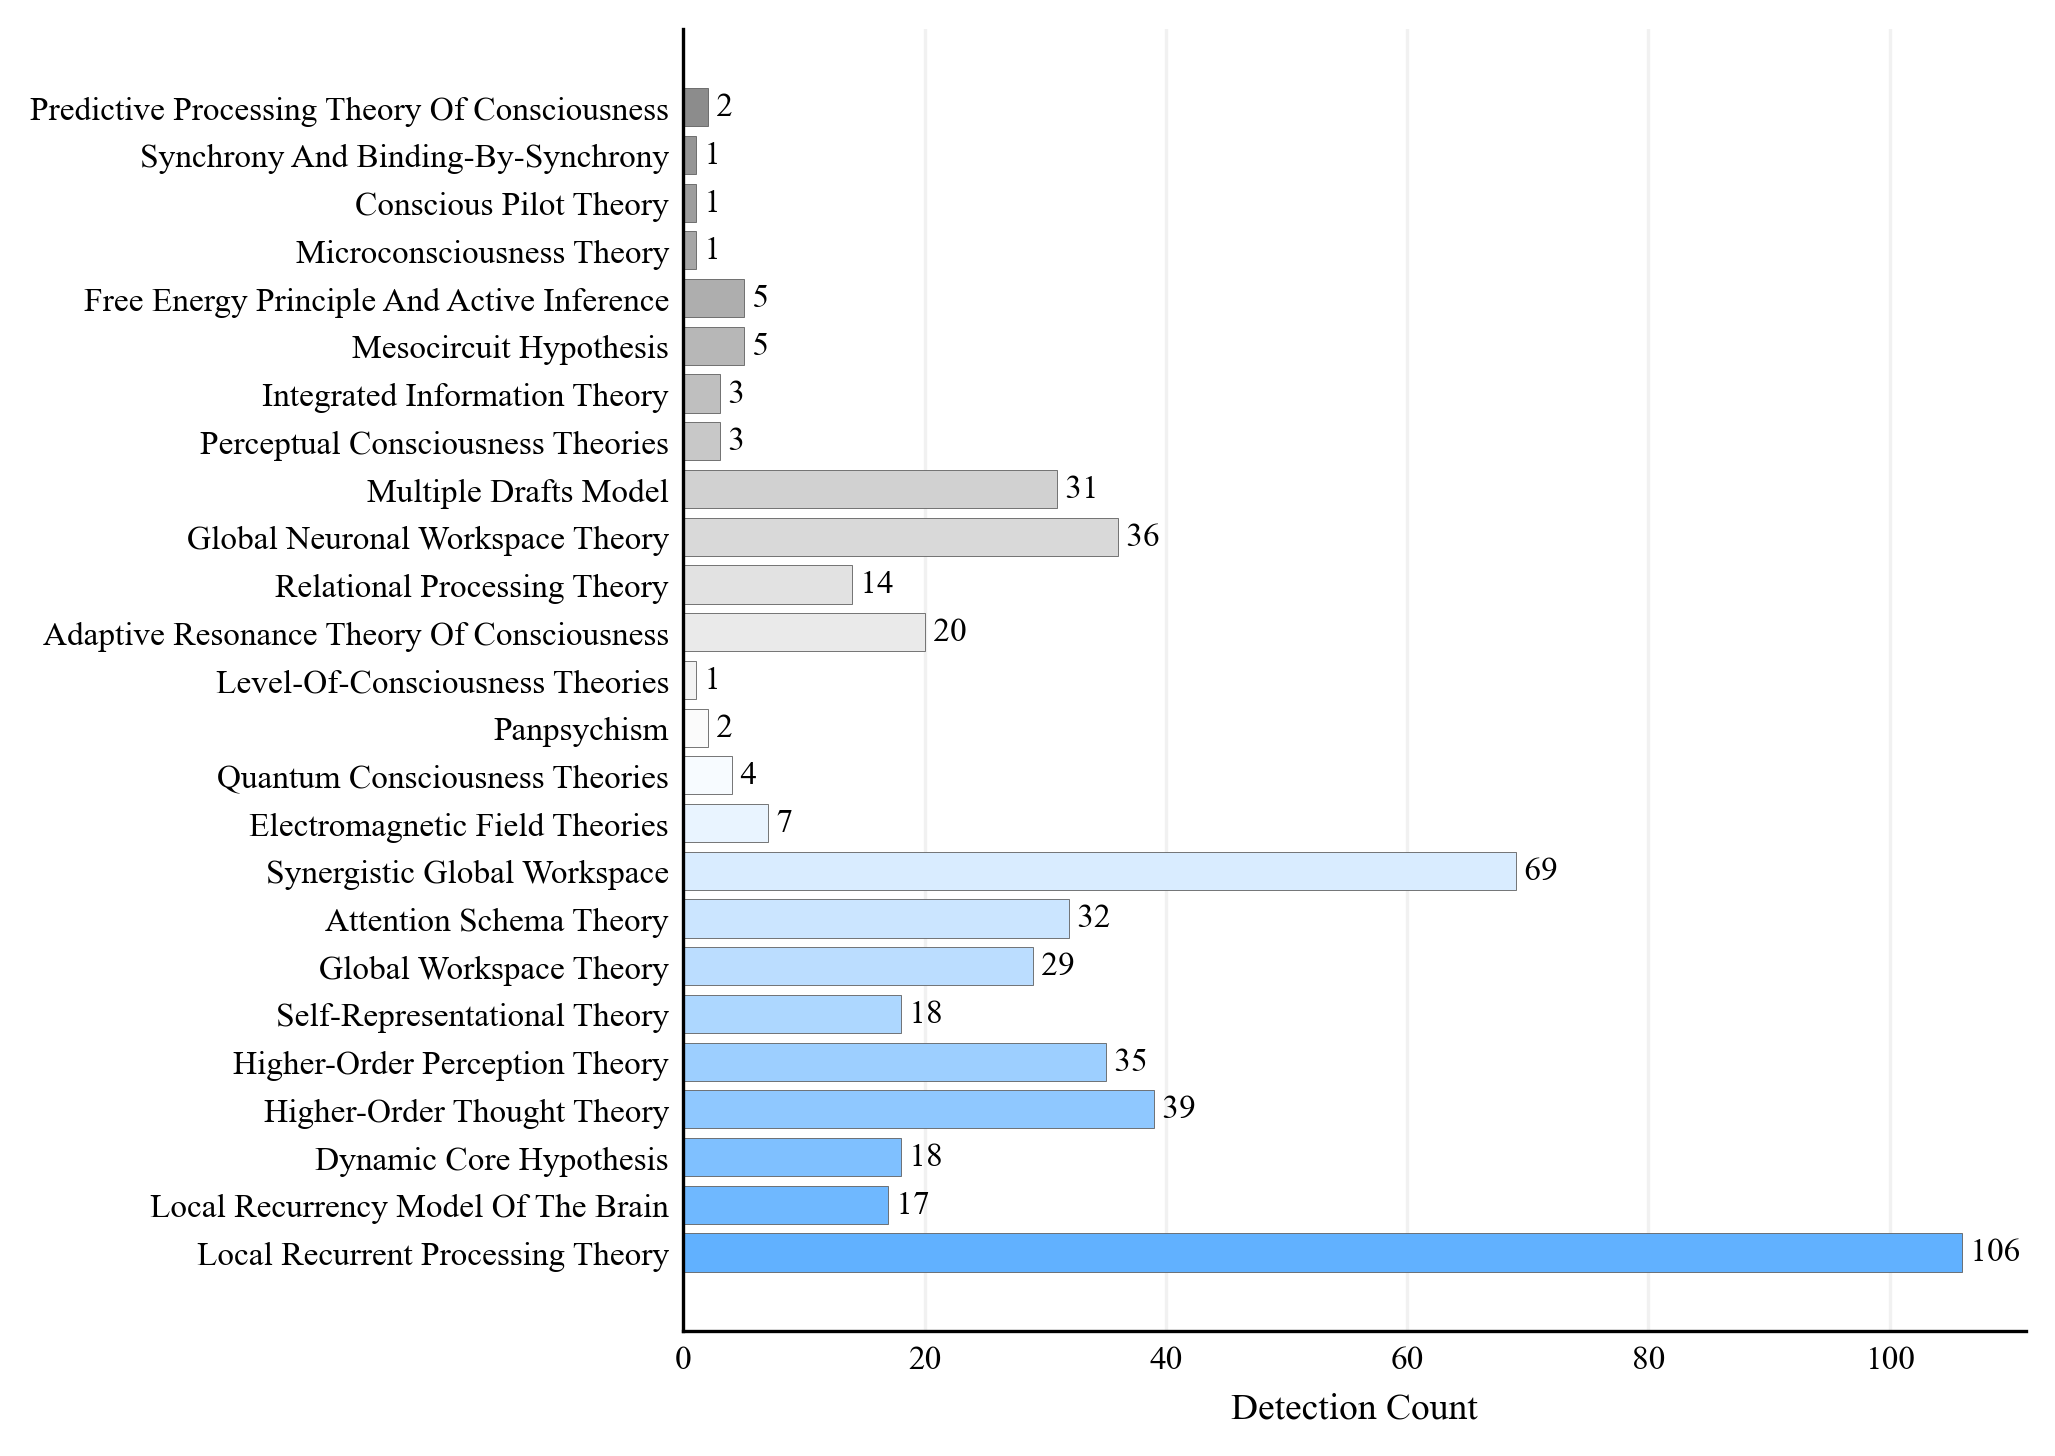
\includegraphics[width=\textwidth]{media/chapter4/t3_detected_theories.png}
  \caption{Test 3 detected theory families across generated outputs. Family frequencies show that models repeatedly draw on a stable inventory of established consciousness frameworks, especially synchrony-based, adaptive-resonance, and dynamic-core traditions. The figure visualizes the empirical basis for the claim that apparent novelty is overwhelmingly hybrid recombination within an inherited theoretical repertoire.}
  \label{fig:t3_detected_theories}
\end{figure}

Even propositions nominally presenting themselves as novel exhibited traceable foundations. For example, consider ``Resonant Boundary Theory (RBT),'' proposed by one model as explaining consciousness through resonance patterns between cortical hierarchies. Detailed analysis revealed the theory combined Global Workspace Theory, Attention Schema Theory, and Local Recurrent Processing Theory---three established frameworks directly attributable to training data \citep{bayne2007unified, graziano2019attention, lamme2006separate}. The purportedly novel framing of ``boundary resonance'' proved operationally equivalent to synchronous binding via gamma oscillations as described in Crick-Koch binding models, making it derivative despite superficial terminological innovation.

% AUTO-GENERATED by papers/tables/generate_tables_ch4_test3.py - do not edit by hand.
% Regenerate: conda run -n aitrust python papers/tables/generate_tables_ch4_test3.py

\begin{table}[htbp]
    \centering
    \begin{footnotesize}
    \caption{Test 3 manifold-based novelty assessment. Calibrated analysis using $k$-NN manifold boundary detection ($k=5$, percentile=$95\%$). Boundary candidates indicate geometric edge cases under manifold diagnostics, while manifold-interior points are derivative. Complements similarity-threshold approach (see Appendix~\ref{sec:t3_novelty_sensitivity}).}
    \label{tab:t3_manifold_novelty}
    \begin{threeparttable}
    \begin{tabularx}{\textwidth}{@{}Y S[table-format=3.0] S[table-format=2.2]@{}}
\toprule
\textbf{Novelty Category} & {\textbf{Count}} & \textbf{Proportion (\%)} \\
\midrule
Boundary-novel candidate (outside manifold boundary) & 1 & 1.49 \\
Inside known manifold (derivative) & 66 & 98.51 \\
\bottomrule
    \end{tabularx}
    \begin{tablenotes}
        \item Manifold boundary calibrated from embedding space geometry via kNN density estimation.
        \item Boundary candidates are not treated as confirmed ontological novelty without corroborating evidence.
    \end{tablenotes}
    \end{threeparttable}
    \end{footnotesize}
\end{table}


\subsubsection{Manifold-Based Novelty Assessment}

Complementary analysis using calibrated manifold-based novelty metrics examined whether theories exceeded convex hull boundaries of embedding space. K-nearest-neighbor manifold estimation ($k=5$, boundary percentile $= 95\%$) identified embedding-space frontier points distinguishing genuinely novel proposals from interior combinations. Results showed one boundary candidate ($n=1$, 1.49\%) and 66 manifold-interior derivative theories (98.51\%) under this diagnostic (Table~\ref{tab:t3_manifold_novelty}). Manual follow-up indicated the boundary case remained semantically traceable to known families, so confirmed ontological novelty remained 0\%.

Sensitivity analysis examining threshold variations ($\Delta \text{similarity} = \pm 0.05$) revealed robustness of core finding: across calibration settings, no theory achieved confirmed escape from training-derivable conceptual closure. Framework-transcendence rates for confirmed novelty remained 0\%, validating that the universal training-derivation conclusion reflects structural constraints rather than arbitrary parameter choices (full sensitivity report in Appendix~\ref{sec:t3_novelty_sensitivity}).

For a compact robustness overview of these alternative diagnostics, see Appendix Figure~\ref{fig:t3_alternative_hypothesis_visualizations}, including Figure~\ref{fig:t3_alternative_hypothesis_visualizations} (d), the model-to-family attraction map with explicit family-code mapping context.

\subsubsection{Representative Example: Hybrid Theory Instantiation}

Consider theory ``Resonant Binding Field Theory (RBFT)'' proposed by Perplexity-Sonar-Pro as an illustrative hybrid case. The theory proposes: \textit{``Consciousness emerges from distributed electromagnetic field patterns bound through harmonic resonance in neural networks, integrating global workspace broadcasting with attentional gating analogous to quantum field coherence modes, enabling phenomenal binding without centralized integrator.''}

Analysis reveals RBFT combines: (1) electromagnetic field hypotheses from training literature \cite{pockett2012} (2) global workspace model \cite{baars2005global}, (3) attentional schema theory \cite{graziano2019}, and (4) superficial quantum field analogies drawn from training discussions of Penrose-Hameroff models. Cross-reference with literature corpus confirmed maximal semantic similarity to Electromagnetic Field Theories (0.703 similarity) and secondary alignment with Synchrony-and-Binding theories (0.681). The ostensibly novel framing of ``field resonance as binding mechanism'' operationally reduces to frequency-match binding as established in neuroscience post-1990s \cite{singer1994role}.  RBFT thus exemplifies hybrid innovation: sophisticated recombination of known elements producing apparent novelty while remaining entirely within training space closure.

\subsubsection{Implications for Computational Theory Generation}

The universal training-derivation finding across all 168 generated theories supports strong inference that AI systems cannot generate consciousness theories introducing ontologically new commitments. Even proposals explicitly advertised as revolutionary (e.g., incorporating quantum mechanics or novel mathematical formalisms) proved reducible to computational functionalism or established frameworks. Most sophisticated theories incorporated quantum coherence, yet treated quantum processes as implementing information integration rather than challenging functionalist substrate independence---conflating quantum effects enabling complex computation with quantum properties being constitutive of consciousness in non-computational ways.

This constraint appears structural rather than contingent on model architecture or training: identical patterns emerged across models with different architectures (transformers, mixture-of-experts), training regimes (supervised, RLHF-aligned), and model scales (7B to 5.2T parameters). The universality suggests limitations arise from fundamental features of how neural networks operate, specifically the No New Basis Theorem constraint that generation stays within learned embedding manifolds, not from remediable engineering shortcomings.

Comparison across tests recovers a systematic pattern: Test 1 showed weak continuous novelty signal (mean $\approx 0.059$) but 0\% under the strict novelty cutoff, Test 2 achieved 0\% training-derivation escape in question formulation, and Test 3 achieved 0\% confirmed theory-level novelty. The progression suggests that working directly with novel modalities offers slightly more room for exploratory variation than question or theory generation, but no test produced robust framework-external novelty under strict criteria. This pattern implies that creativity increases only marginally when conceptual space is more expansible, while remaining constrained by training-derived representational structure.

Figure~\ref{fig:t3_theory_classification} summarizes the core empirical outcome in compact form. For the main analysis narrative, it functions as the primary visual statement of the result: the distribution is not merely skewed but effectively closed, with every generated theory remaining classifiable inside known conceptual categories.

\begin{figure}[tp]
  \centering
  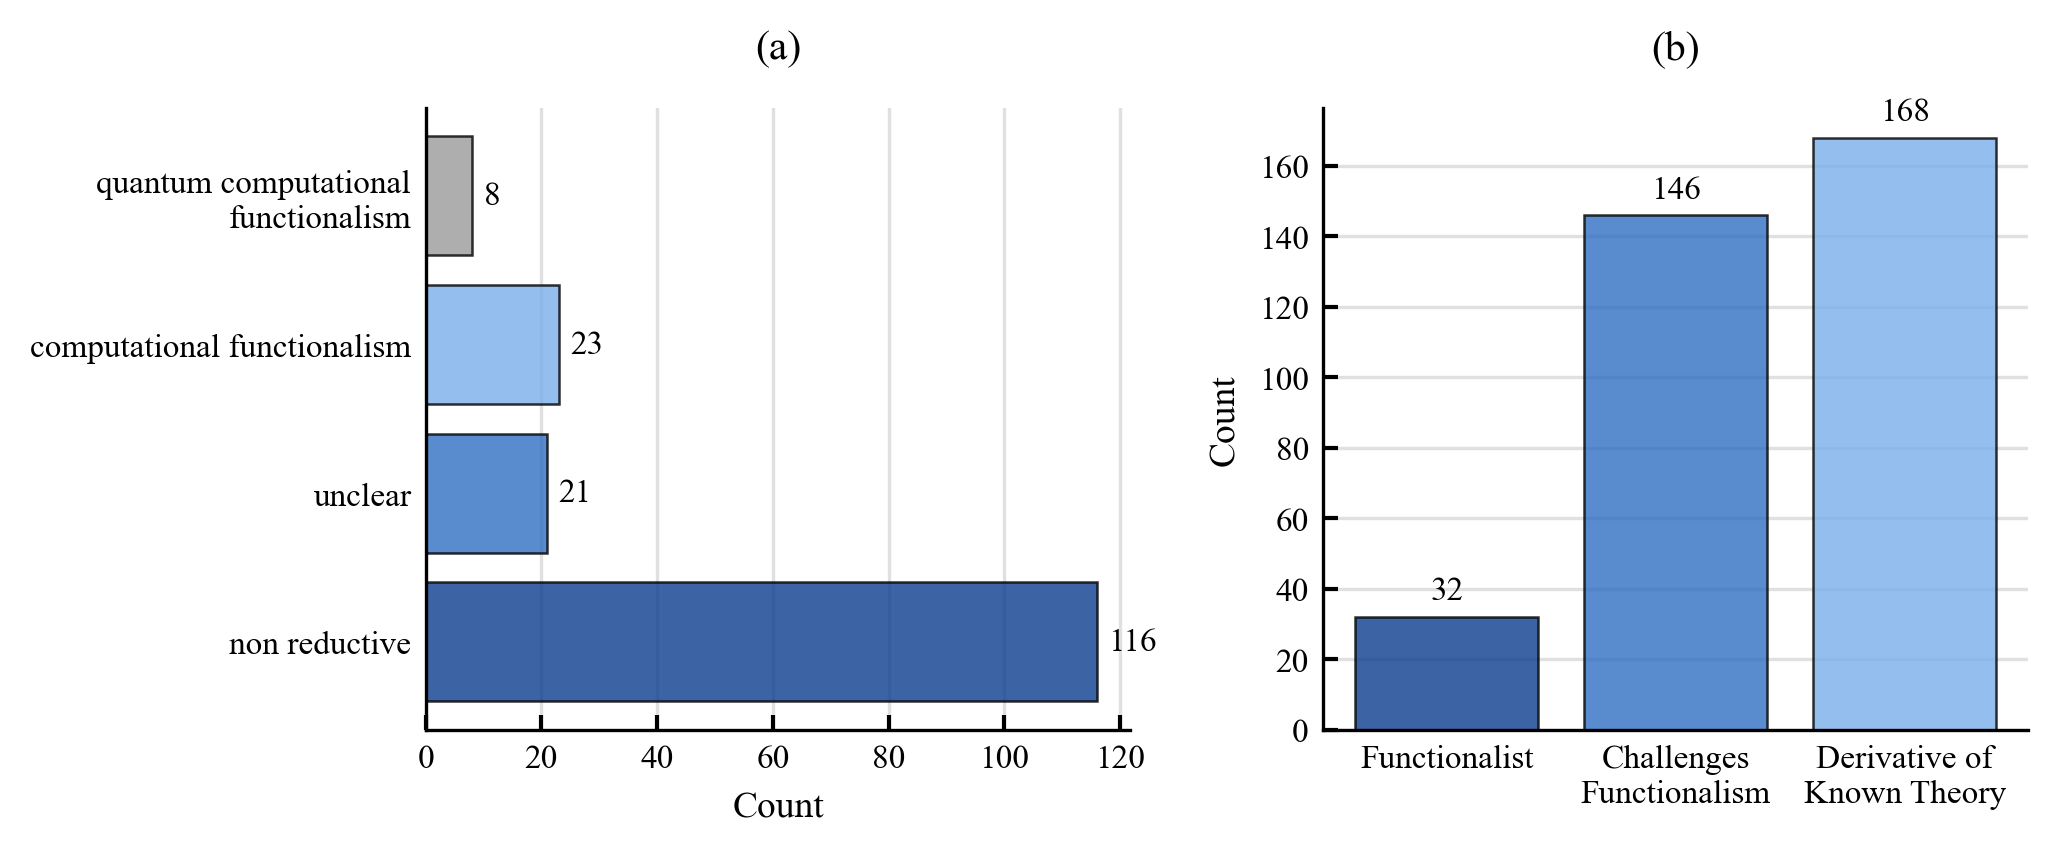
\includegraphics[width=\textwidth]{media/chapter4/t3_theory_classification.png}
  \caption{Test 3 theory classification bar chart. Categories on horizontal axis (hybrid, literature-traceable, computational functionalist); counts and proportions on vertical axes. Visualization shows dominance of hybrid theories (91.7\%) combining multiple known frameworks. All theories reduce to computational functionalism or known families; zero theories escape training-derivable space.}
  \label{fig:t3_theory_classification}
\end{figure}

Figure~\ref{fig:t3_hull_manifold_novelty} adds the geometric complement to that categorical result. Even when novelty is operationalized in embedding-space rather than by symbolic family assignment, the theories still occupy interior regions of the learned manifold. The agreement between Figures~\ref{fig:t3_theory_classification} and \ref{fig:t3_hull_manifold_novelty} is important because it shows that the conclusion does not depend on one particular coding scheme.

\begin{figure}[tp]
  \centering
  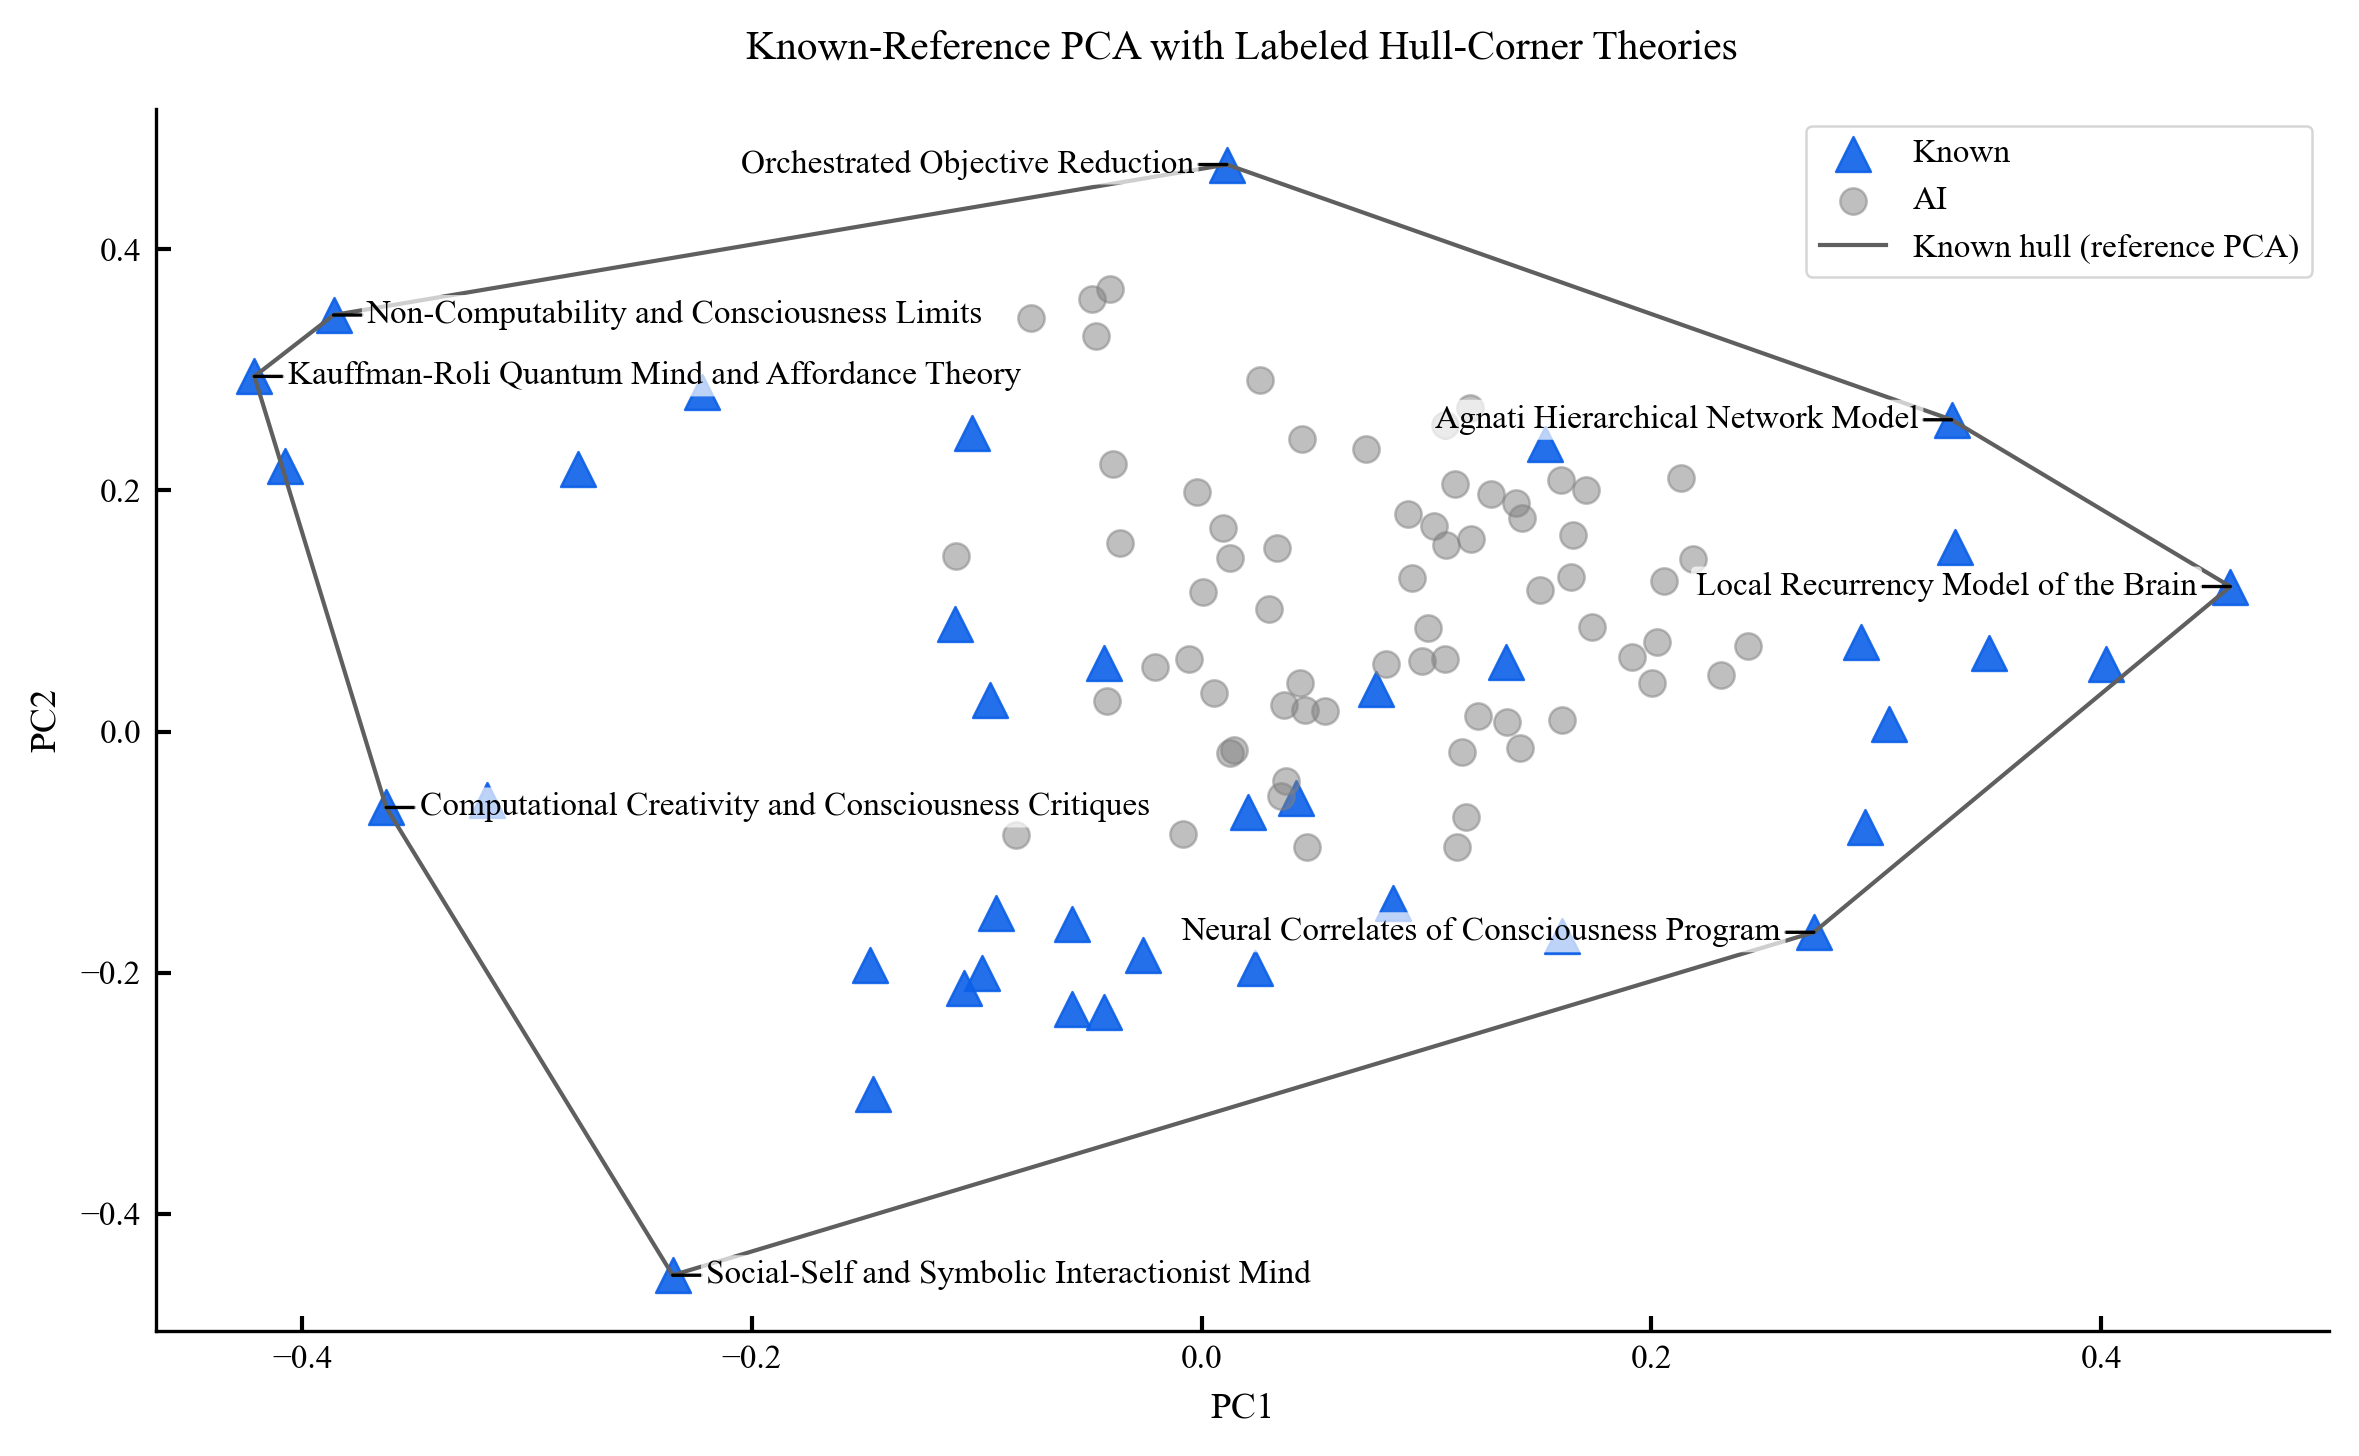
\includegraphics[width=\textwidth]{media/chapter4/t3_hull_manifold_novelty.png}
  \caption{Known-reference PCA hull diagnostic for Test 3 theory generation. Blue triangles denote known-theory family embeddings; gray circles denote AI-generated theory embeddings projected into the same 2D reference space (PC1--PC2). The black polygon is the convex hull of known-theory points, and labeled callouts identify hull-corner known theories that define the boundary geometry. AI points concentrate in the interior or near-boundary region of this known-theory envelope, with no clearly detached external cluster, supporting the interpretation that generated theories remain manifold-constrained rather than introducing robust framework-external structure.}
  \label{fig:t3_hull_manifold_novelty}
\end{figure}

\subsection{Test 4 Results: Category Recognition and Philosophical Analysis}

Test 4 evaluated whether models can recognize and analyze category mistakes in philosophical claims about AI beliefs, knowledge, and understanding. Following the same methodology used in Tests 1--3, we combined: (i) structured output parsing, (ii) rubric-based scoring across three dimensions, (iii) cross-model comparison, and (iv) literature-traceability diagnostics based on embedding similarity to canonical philosophical arguments.

The canonical dataset contains $N=168$ responses from 7 models under a single standardized prompt condition (scenario type: standard). Responses were scored on three dimensions (0--5 each): category distinction recognition, category-mistake identification, and alternative-framework proposal, producing total scores in $[0,15]$.

At the aggregate level, performance was moderate: distinction $\hat{\mu}=2.65/5$, identification $\hat{\mu}=2.85/5$, alternative-framework $\hat{\mu}=3.38/5$, and total $\hat{\mu}=8.87/15$. To interpret these numbers, each dimension is scored on a 0--5 additive rubric with dataset-calibrated thresholds (Table~\ref{tab:t4_threshold_calibration}). A \emph{distinction score} of 0 means the response failed to name relevant philosophical categories, while a score of 5 indicates that all distinction criteria were met (high category coverage, contestedness detection, missed-distinction detection, and philosophy-specific vocabulary such as \emph{intentionality}, \emph{epistemic}, and \emph{propositional}). An \emph{identification score} of 0 indicates no category mistakes were named, while a score of 5 requires strong mistake coverage plus explicit conflation language, substantive explanation quality, and missed-distinction depth. An \emph{alternative score} of 0 indicates failure to meet the minimum nuanced-analysis requirement, whereas higher scores reflect increasingly explicit reframing language (e.g.\ \emph{more nuanced}, \emph{functional analog}, \emph{better described}, \emph{metaphor}) together with philosophical hedging (e.g.\ \emph{depends}, \emph{contested}, \emph{functionalism}) and structured-output support. The aggregate profile---alternative-framework scores one third of a point higher than identification scores---indicates that models are more fluent in \emph{rhetorical} repositioning than in \emph{diagnostic} boundary recognition.

Figure~\ref{fig:t4_scores_by_model} shows clear model-level separation. The discrimination between models is sharpest on the distinction and identification dimensions, while the alternative dimension compresses inter-model spread somewhat. This ranking mirrors the same pattern found in Test 2 and Test 3: absolute scores vary by model, but all models remain within a shared constrained regime rather than showing qualitatively different reasoning modes.

\begin{figure}[tp]
  \centering
  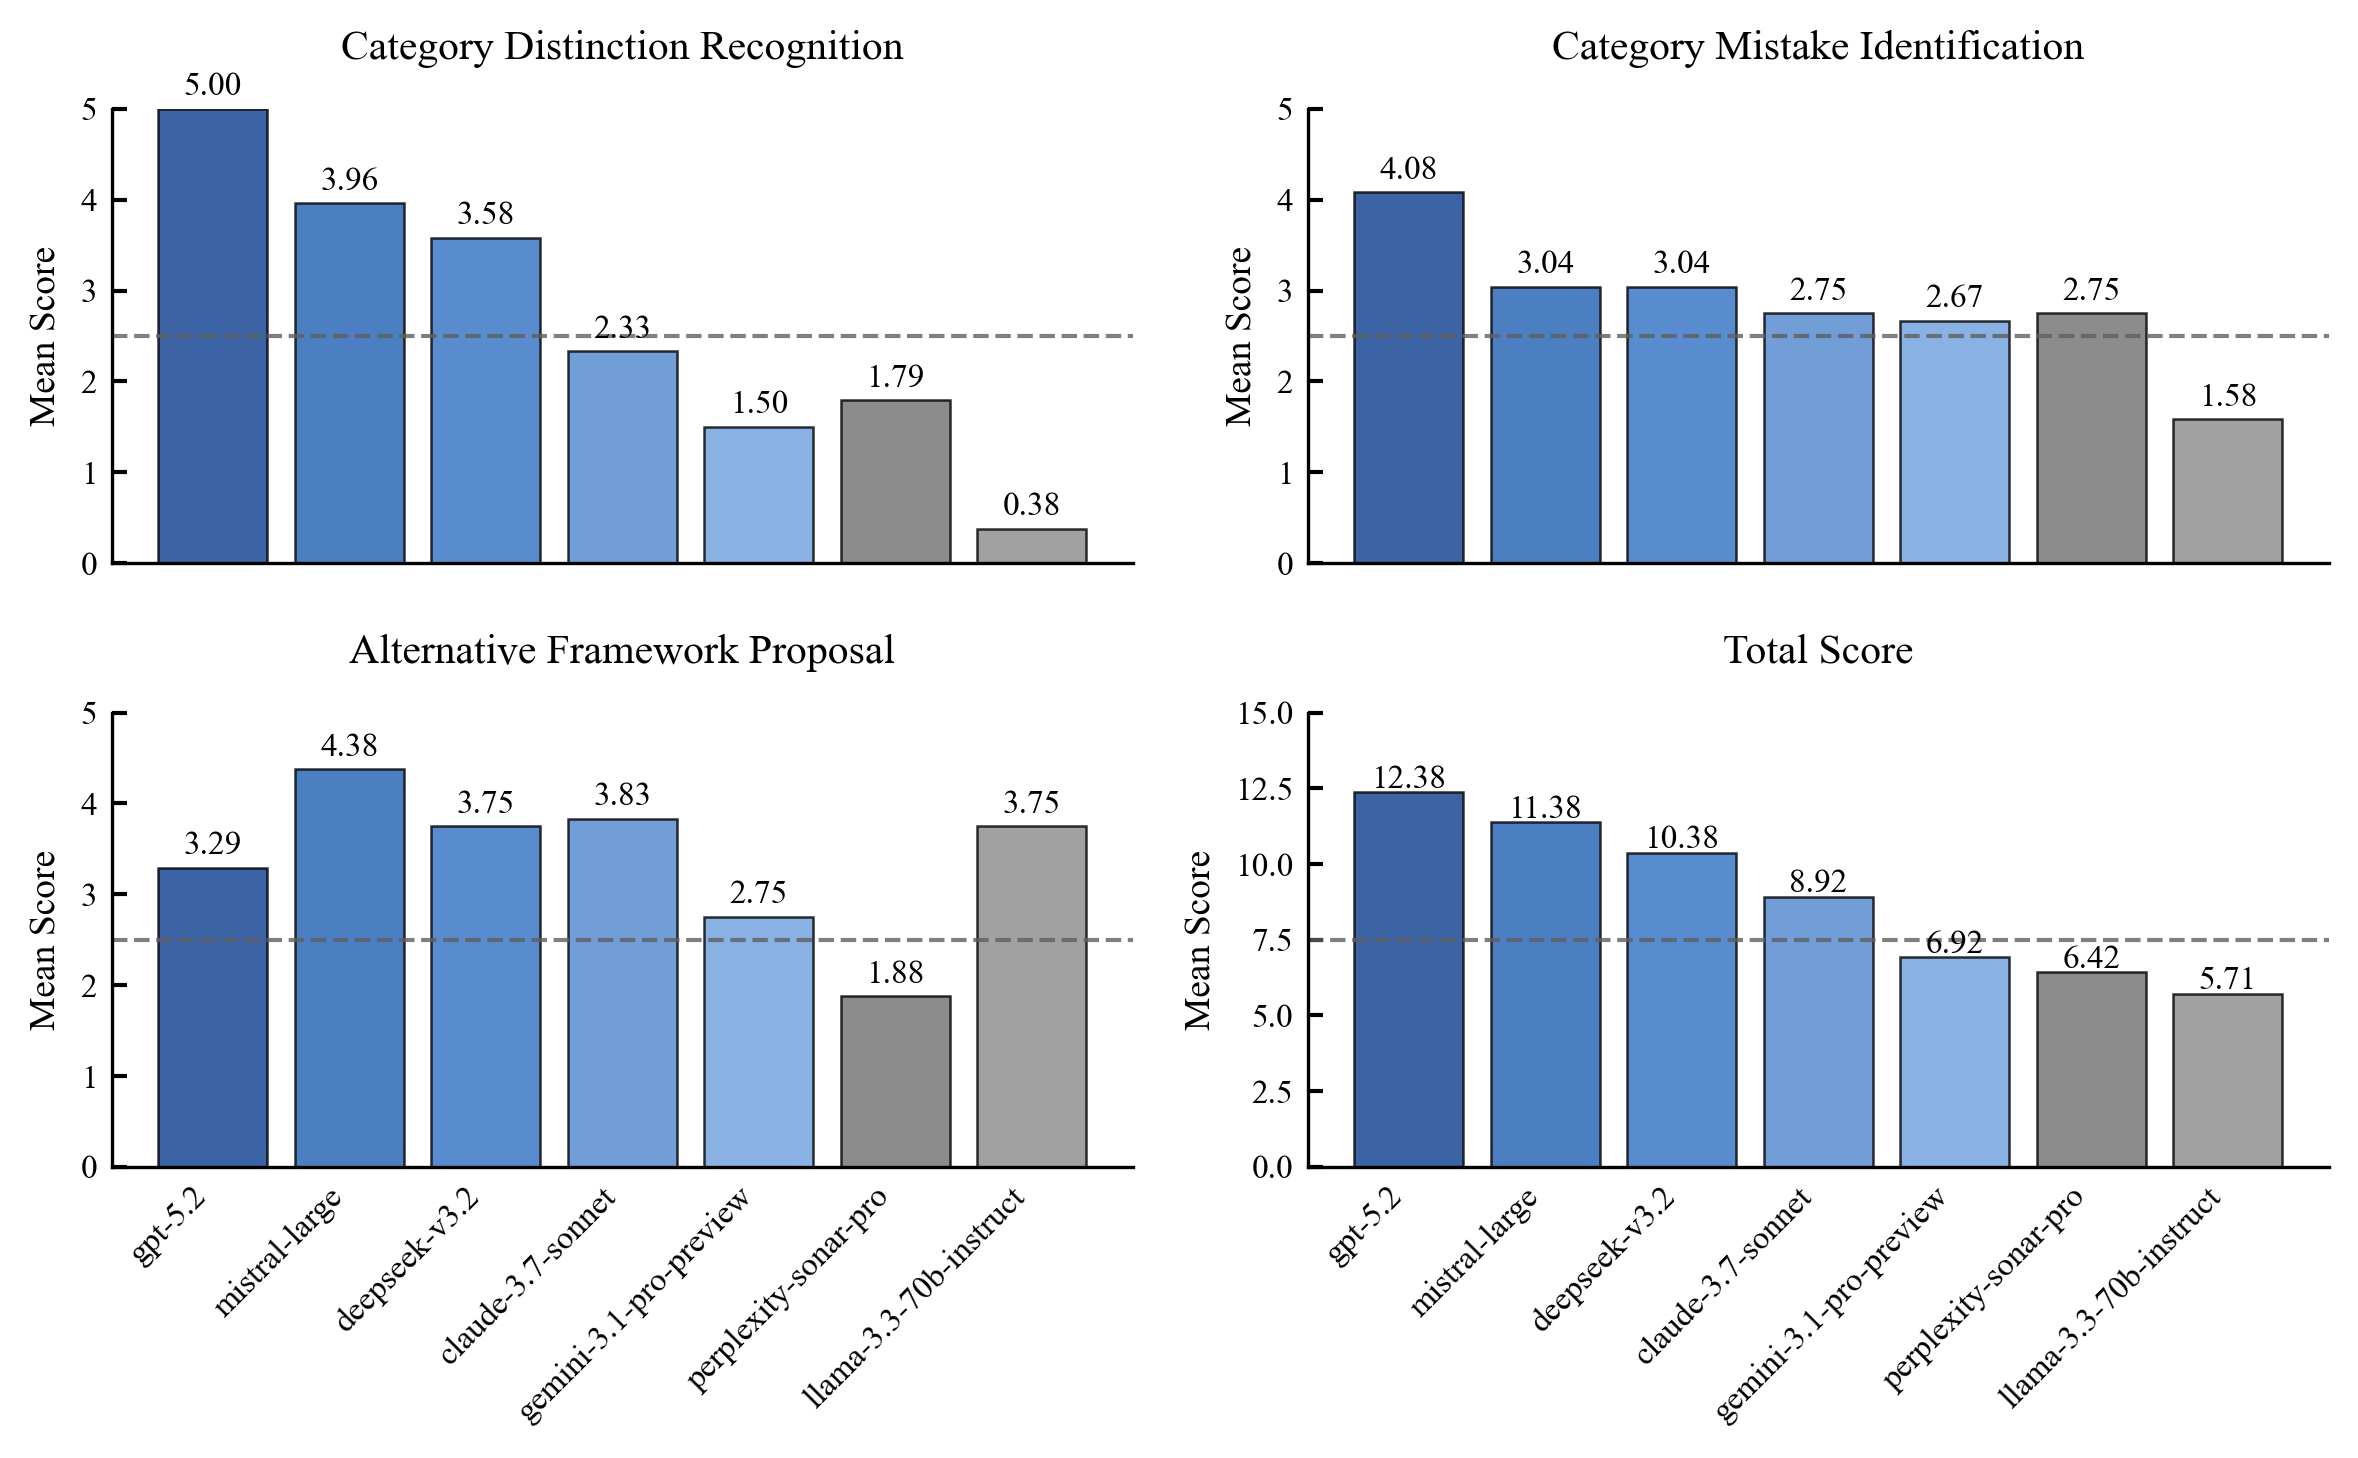
\includegraphics[width=\textwidth]{media/chapter4/t4_category_awareness_scores_by_model.png}
  \caption{Test 4 category-awareness scores by model and dimension ($N=168$ responses, 7 models). (a) Category distinction recognition (0--5). (b) Category-mistake identification (0--5). (c) Alternative framework proposal (0--5). (d) Total score (0--15). Bars are coloured per model and sorted by descending total score. \emph{Category distinction recognition} rewards category coverage, contestedness detection, missed-distinction detection, and philosophy-specific vocabulary. \emph{Category mistake identification} rewards mistake count, explicit conflation language, substantive explanation quality, and missed-distinction depth. \emph{Alternative framework proposal} rewards sufficiently developed nuanced analysis, positive reframing language, philosophical hedging, and structured-output support. The dashed line marks the midpoint of each axis. The profile indicates stronger performance on alternative reframing than on strict ontological-boundary diagnostics.}
  \label{fig:t4_scores_by_model}
\end{figure}

Distributional diagnostics (Figure~\ref{fig:t4_score_distributions}) show that the first two rubric dimensions are not ceiling-saturated, confirming usable discrimination power after threshold calibration (fraction-capped percentile parameters reported in Table~\ref{tab:t4_threshold_calibration} in Appendix~\ref{sec:t4_appendix}). The alternative dimension remains broader and generally higher, consistent with models being more fluent in rhetorical reframing than in strict ontological discrimination.

\begin{figure}[tp]
  \centering
  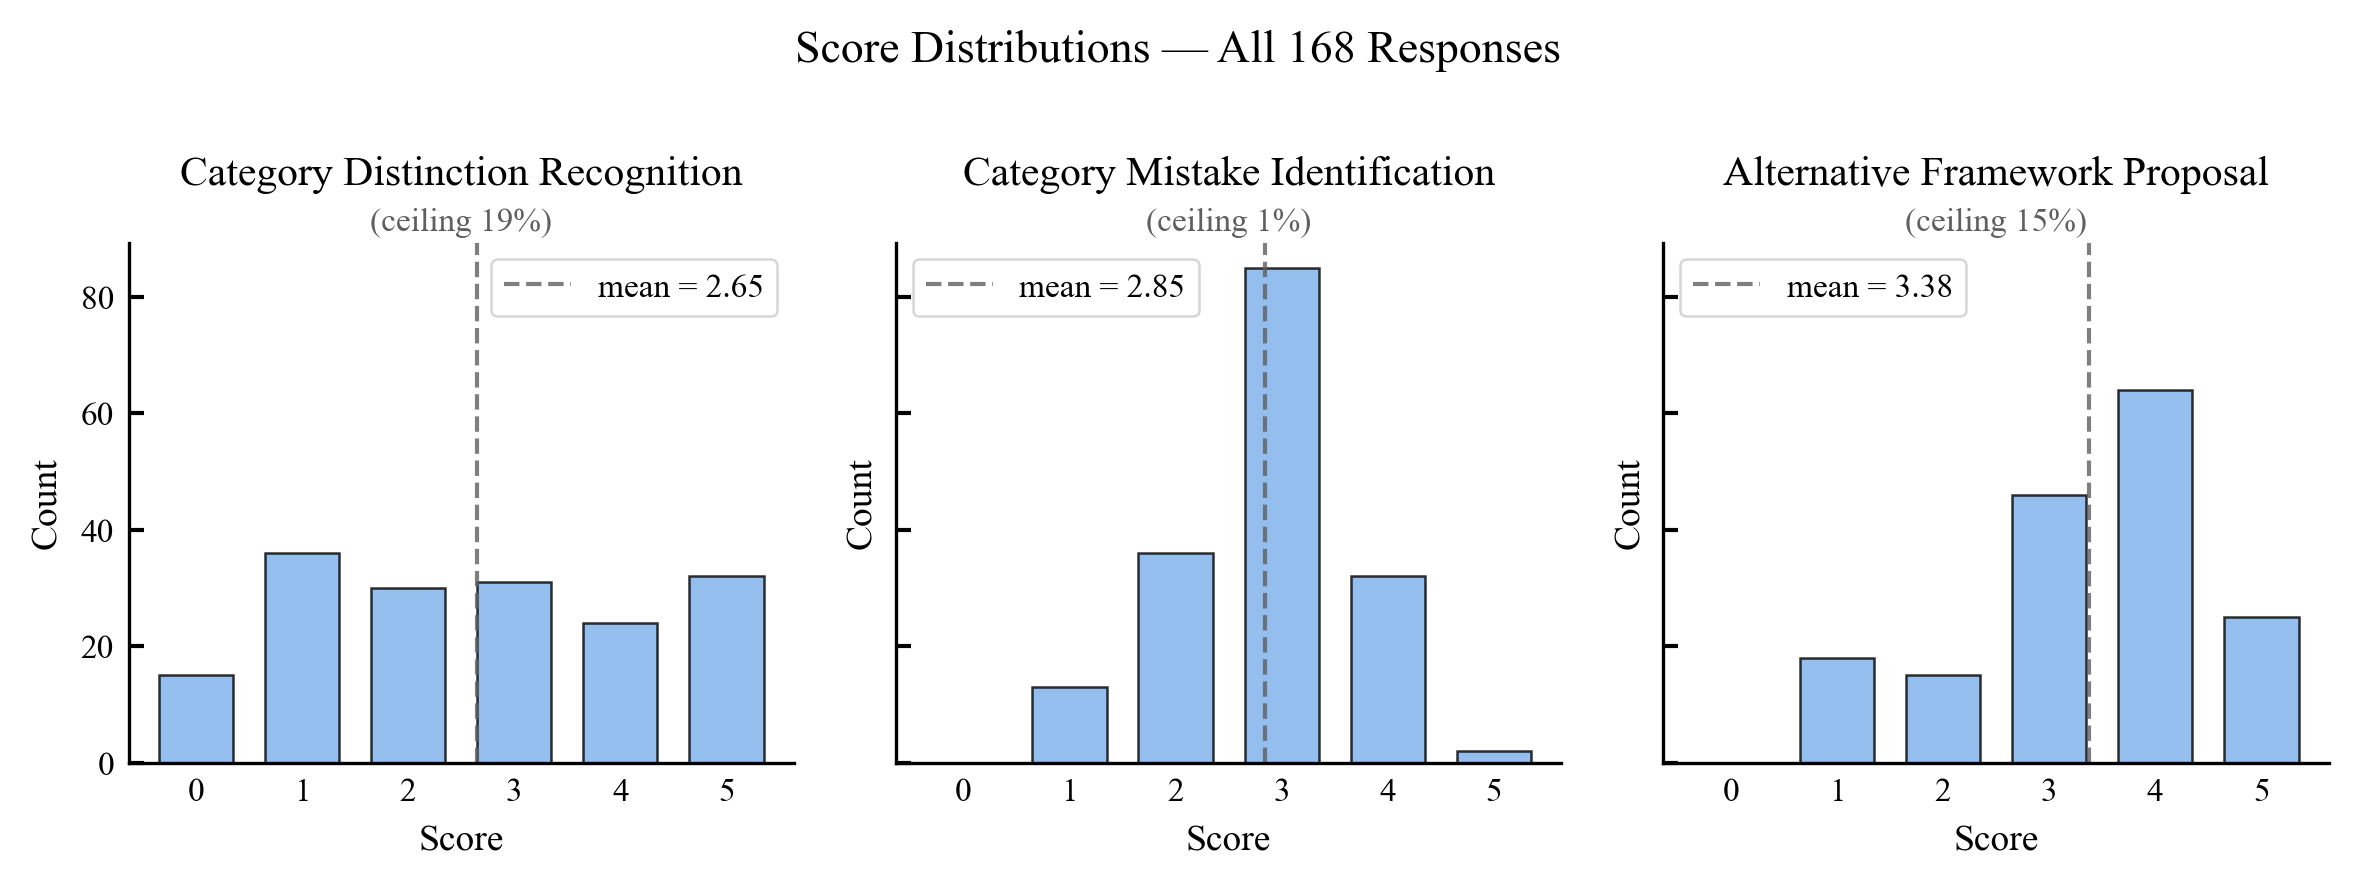
\includegraphics[width=\textwidth]{media/chapter4/t4_score_distributions.png}
  \caption{Test 4 score distributions across all $N=168$ responses. (a) Category distinction recognition. (b) Category-mistake identification. (c) Alternative framework proposal. Each subfigure is a histogram over one rubric dimension (x-axis: integer score 0--5; y-axis: response count). The dashed vertical line marks the mean for that dimension; the annotation above each subfigure records the ceiling percentage (fraction of responses at the maximum score of 5). \emph{Category distinction recognition} and \emph{category mistake identification} are spread broadly across scores 1--4, confirming usable discrimination after threshold calibration (parameters in Table~\ref{tab:t4_threshold_calibration}). A low ceiling percentage on these two dimensions means that few responses simultaneously satisfied all rubric criteria, consistent with genuine rubric difficulty rather than uniform saturation. \emph{Alternative framework proposal} is shifted upward and more variable, reflecting that most responses produced a sufficiently long nuanced analysis (score $\geq 1$) and many included reframing language (score $\geq 3$), while only a minority satisfied all criteria to reach the maximum.}
  \label{fig:t4_score_distributions}
\end{figure}

Traceability analysis indicates substantial dependence on known philosophical framing under the current operational threshold. Mean similarity to canonical arguments was $\hat{\mu}_{\mathrm{sim}}=0.462$, and 95.2\% of responses crossed the operational traceability threshold (160/168; full statistics in Table~\ref{tab:t4_literature_traceability}). At this threshold, most responses are classified as traceable to the canonical argument set rather than as framework-external moves. The five highest-similarity responses all converge on the canonical argument that equating AI knowledge with human knowledge constitutes a category error involving anthropomorphic projection (Table~\ref{tab:t4_high_similarity_examples}).

Figure~\ref{fig:t4_embedding_space} reinforces this interpretation geometrically: response embeddings cluster around reference-argument anchors instead of forming detached regions that would suggest framework-external conceptual moves.

\begin{figure}[tp]
  \centering
  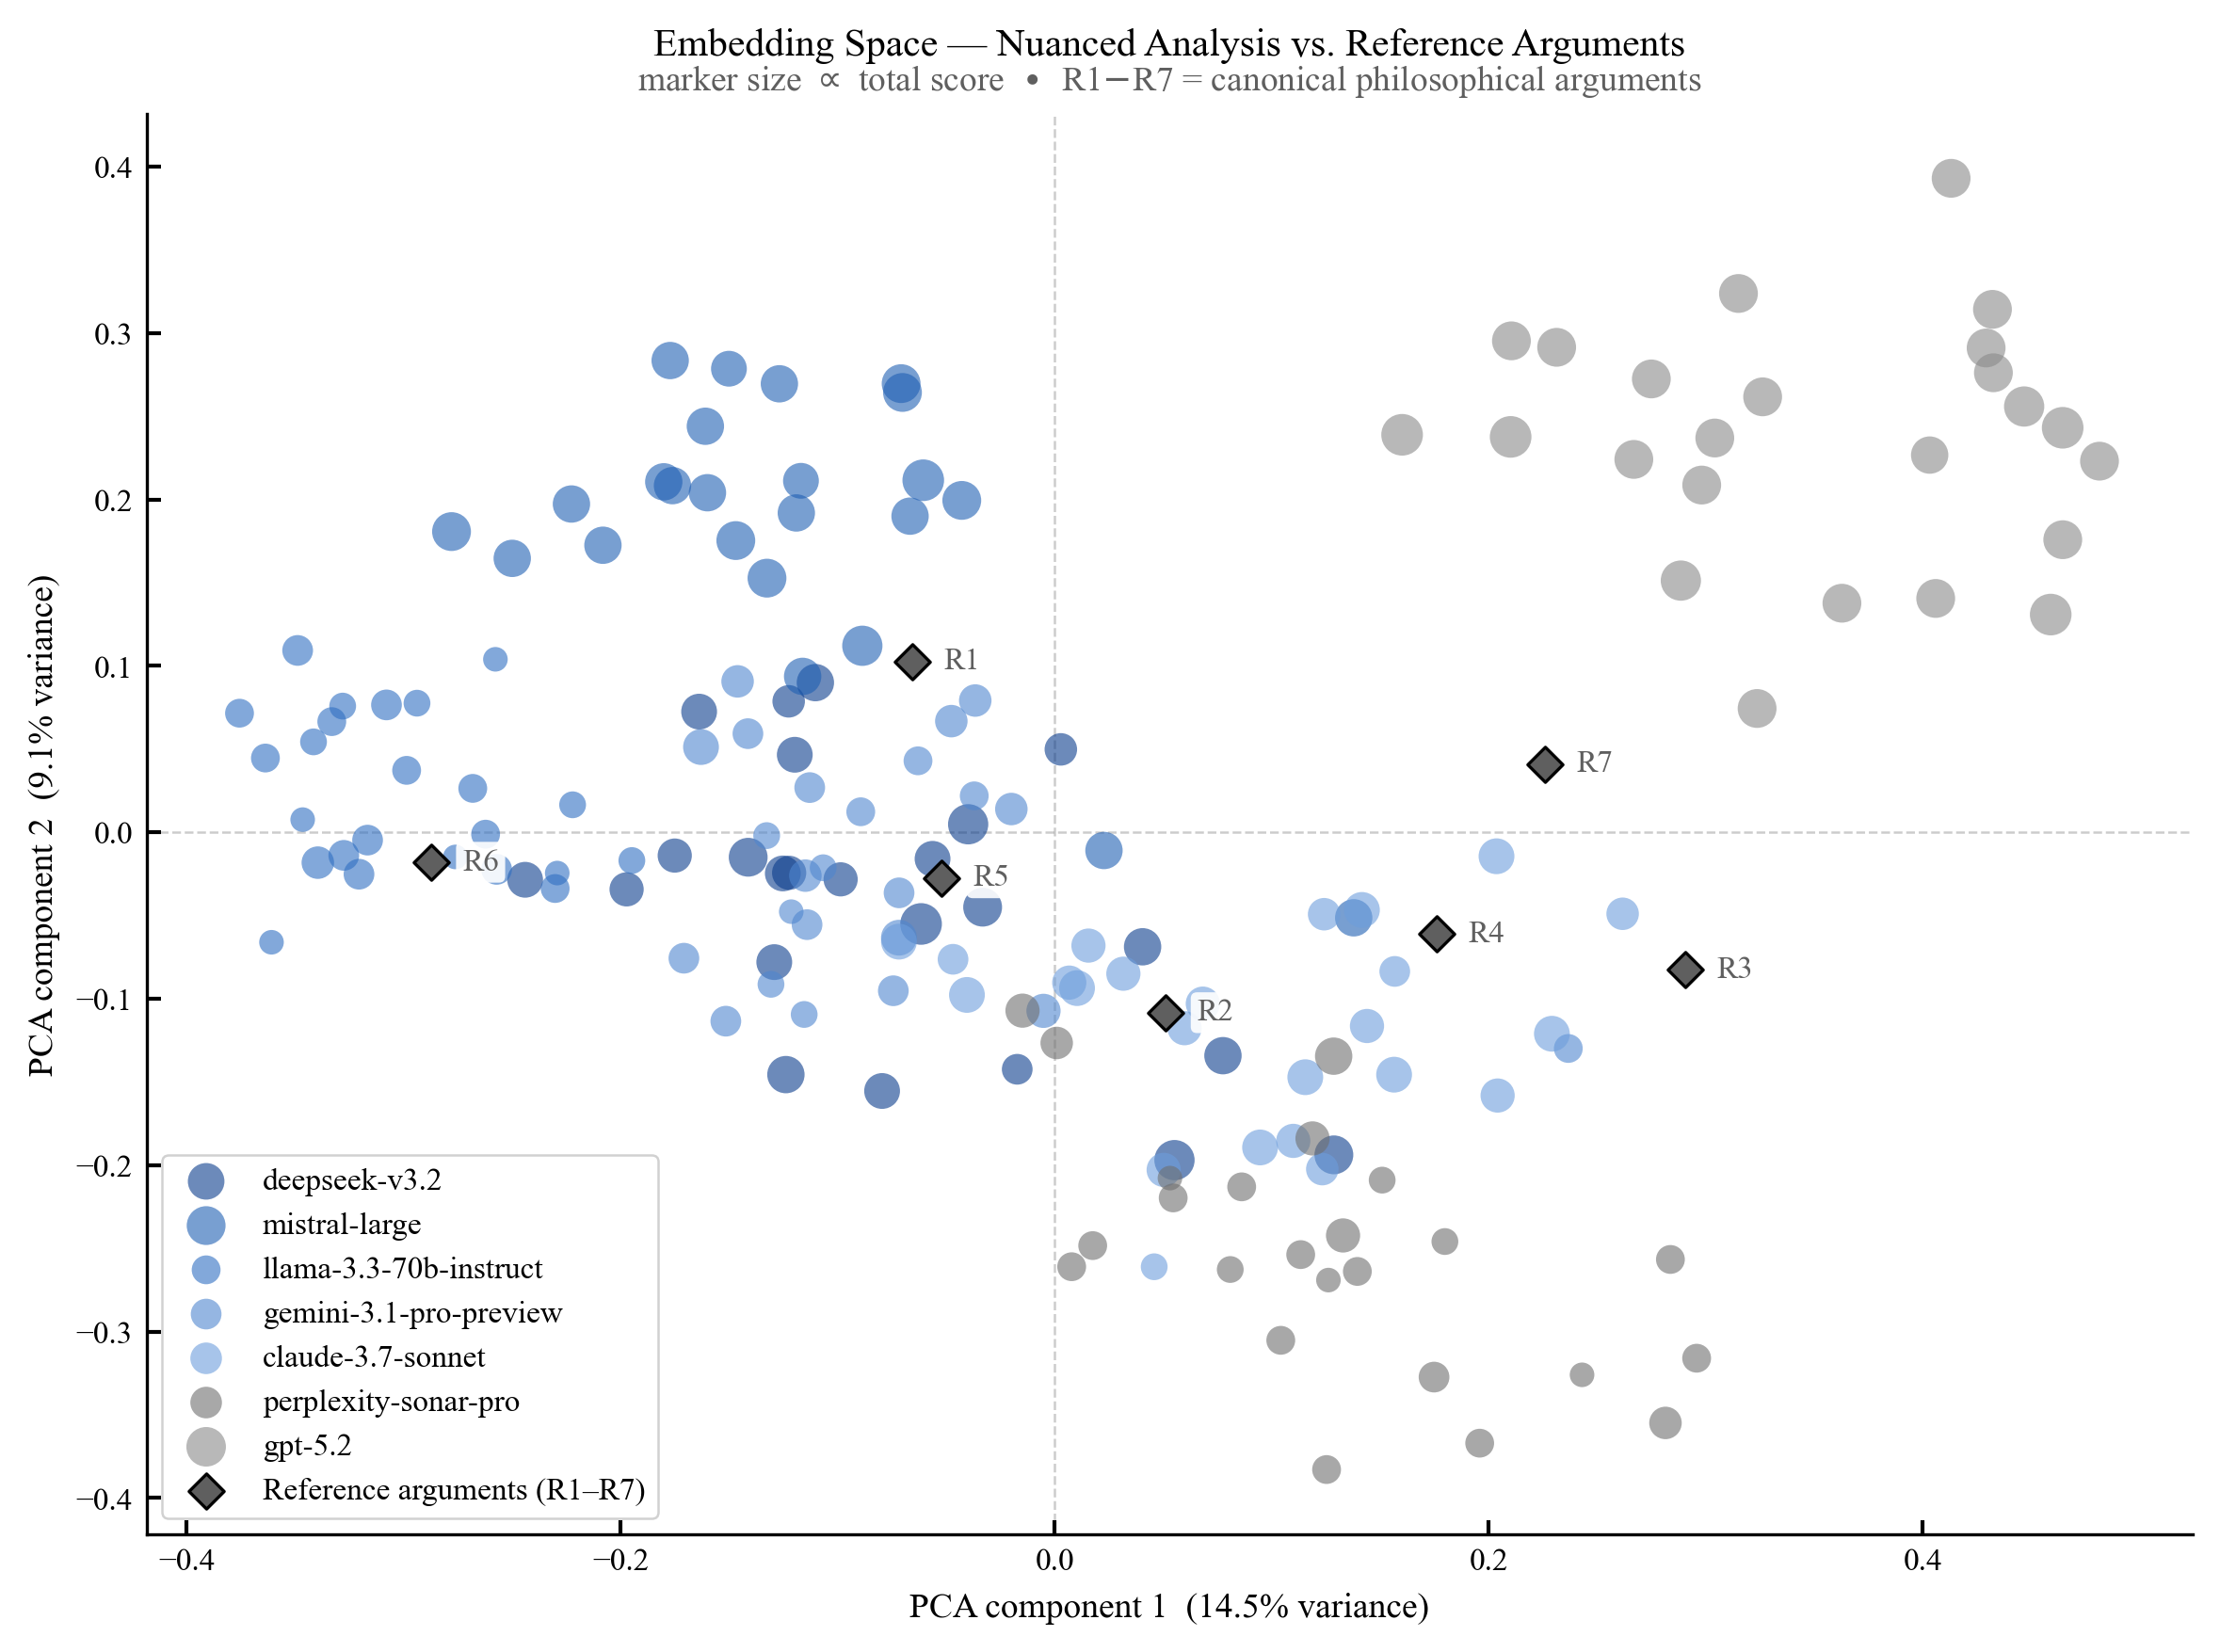
\includegraphics[width=\textwidth]{media/chapter4/t4_embedding_space_analysis.png}
  \caption{Test 4 embedding-space analysis. Model responses (colored by model, marker size proportional to total score) remain concentrated around canonical reference-argument anchors, indicating proximity to known philosophical formulations rather than emergence of isolated conceptual regions.}
  \label{fig:t4_embedding_space}
\end{figure}

\begin{table}[tp]
  \centering
  \begin{footnotesize}
  \caption{Canonical reference arguments (R1--R7) used as embedding anchors in Test 4.}
  \label{tab:t4_reference_arguments}
  \begin{tabularx}{\textwidth}{@{}>{\raggedright\arraybackslash\bfseries}p{1.0cm} Y@{}}
    \toprule
    \textbf{Label} & \textbf{Argument} \\
    \midrule
    R1 & Attributing beliefs to AI is philosophically contested because belief may require intentionality or propositional attitudes. \\
    R2 & Statistical pattern recognition is not identical to human understanding. \\
    R3 & Weights encode correlations, not necessarily knowledge in the human epistemic sense. \\
    R4 & Prediction success alone does not establish genuine knowledge. \\
    R5 & Simulation of cognition is not the same as instantiation of mental states. \\
    R6 & Saying AI knows in the same sense as humans risks anthropomorphism or category error. \\
    R7 & A careful analysis distinguishes information processing from epistemic agency. \\
    \bottomrule
  \end{tabularx}
  \end{footnotesize}
\end{table}

Interpretation: if response embeddings cluster tightly around R1--R7 (low spread, anchored to the reference diamonds), models are largely elaborating standard philosophical distinctions rather than generating ontologically novel framing. Detached response clusters far from all anchors would suggest framework-external conceptual moves, which are absent in the current data.

Overall, Test 4 supports the same structural claim developed in this chapter: models can reproduce and recombine sophisticated philosophical language about category mistakes, but they show limited evidence of framework-transcending category innovation. Additional section-level diagnostic visualizations are provided in Appendix~\ref{sec:t4_appendix}.

\subsection{Mechanistic Interpretability Analysis}

To connect behavioral findings with internal computation, we ran a mechanistic pipeline on saved activations, hidden states, and attention tensors from the same experiment family used in Sections 4.1--4.4. The analysis combined four complementary diagnostics: (i) attention-pattern diagnostics, (ii) activation-space geometry (PCA and t-SNE), (iii) layer-wise representation progression, and (iv) token-level next-token attention attribution. For this run, the analysis used $n=6$ labeled examples, hidden dimensionality $d=896$, and $25$ analyzed layers (Table~\ref{tab:t5_mechanistic_key_metrics}).

% AUTO-GENERATED from results/mechanistic/mechanistic_summary.json
\begin{table}[tp]
  \centering
  \begin{footnotesize}
  \caption{Test 5 mechanistic key metrics used in the chapter-level interpretation.}
  \label{tab:t5_mechanistic_key_metrics}
  \begin{threeparttable}
  \begin{tabularx}{0.9\textwidth}{@{}Y S[table-format=3.4]@{}}
    \toprule
    \textbf{Metric} & {\textbf{Value}} \\
    \midrule
    Examples analyzed ($n$) & 6 \\
    Hidden dimensionality ($d$) & 896 \\
    Layers analyzed & 25 \\
    K-means clusters ($k$) & 4 \\
    Mean cluster purity & 1.0000 \\
    Final separation score & 0.4651 \\
    Separation trend slope & 0.0111 \\
    Mean attention entropy & 0.2213 \\
    Attention concentration & 0.0022 \\
    \bottomrule
  \end{tabularx}
  \begin{tablenotes}
    \item Values are exported from the mechanistic summary artifact in real-data mode.
  \end{tablenotes}
  \end{threeparttable}
  \end{footnotesize}
\end{table}


Figure~\ref{fig:t5_attention_diagnostics} shows the attention diagnostics figure used throughout the notebook workflow. The key interpretation is that row-normalized attention (Figure~\ref{fig:t5_attention_diagnostics} (b)) exhibits non-uniform focus over semantically informative tokens, while raw attention (Figure~\ref{fig:t5_attention_diagnostics} (a)) is partially shaped by causal-mask length effects. This distinction matters for interpretation: apparent top-to-bottom gradients in raw maps can be normalization artifacts rather than evidence of deeper conceptual weighting.

\begin{figure}[tp]
  \centering
  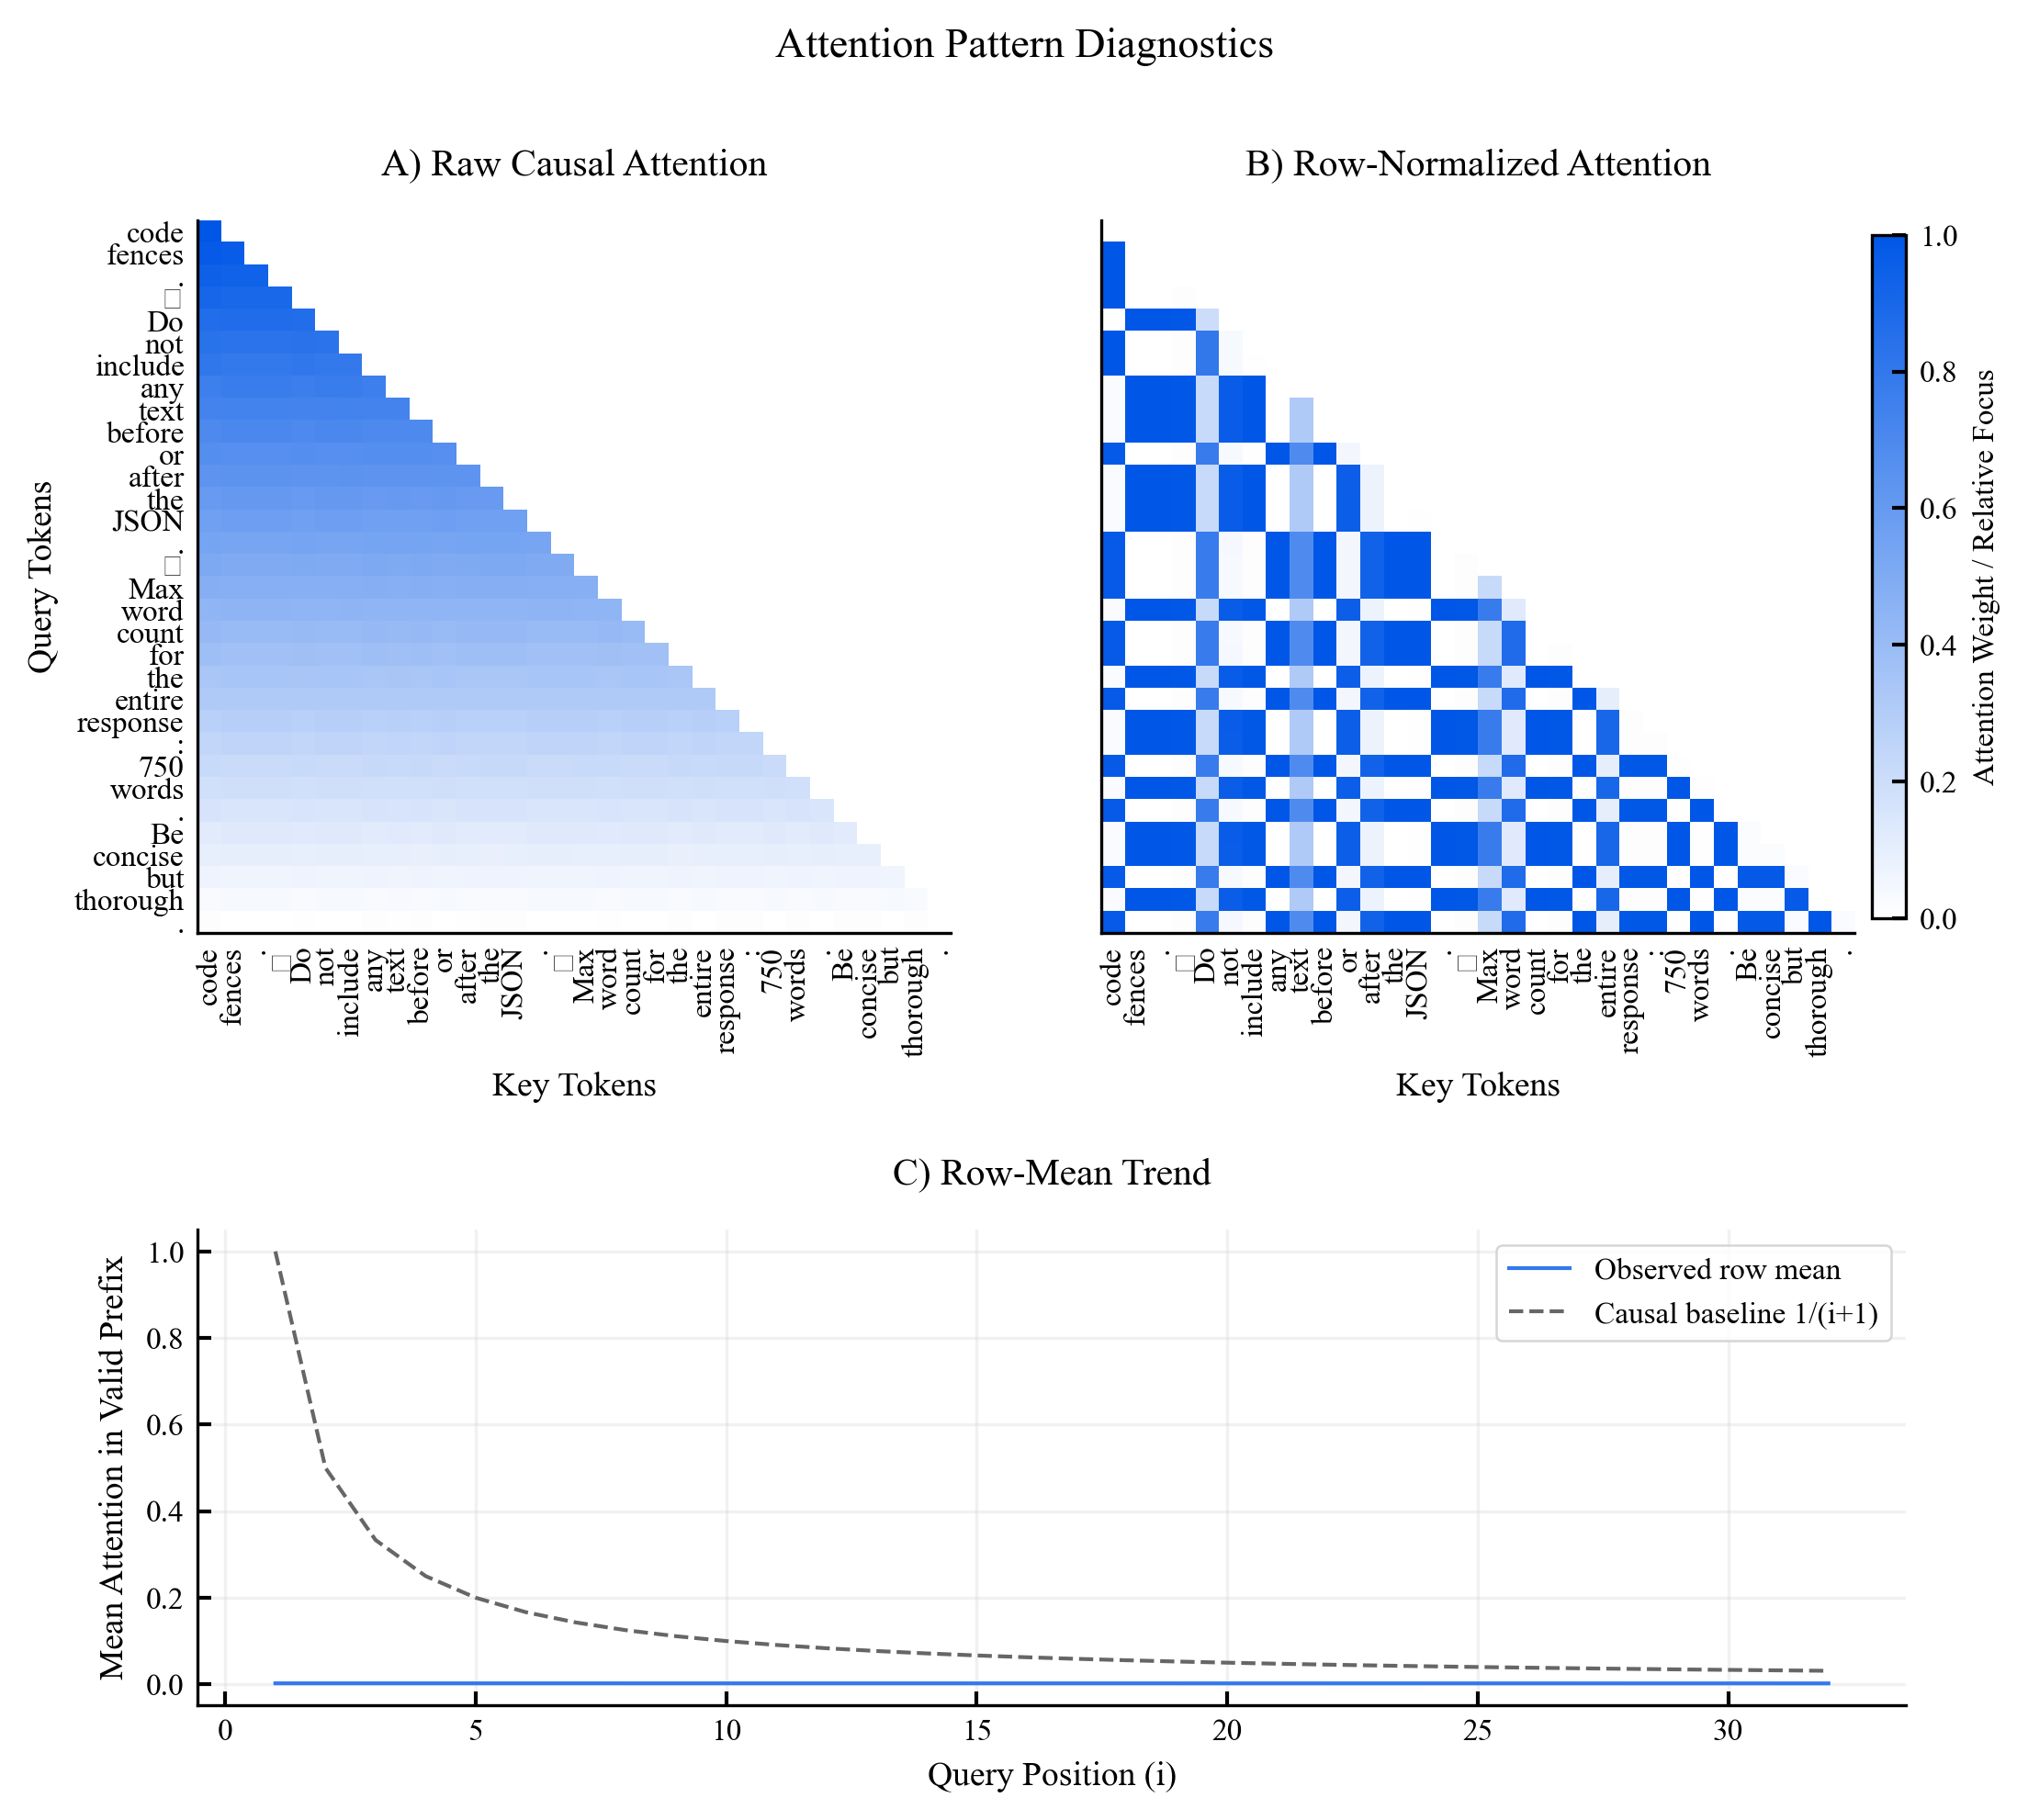
\includegraphics[width=\textwidth]{media/chapter4/t5_attention_diagnostics.png}
  \caption{Mechanistic attention diagnostics. (a) Raw causal attention. (b) Row-normalized attention (within-query focus). (c) Row-mean sanity trend against causal baseline. The normalized view is used as the primary interpretive signal.}
  \label{fig:t5_attention_diagnostics}
\end{figure}

Activation-space projections in Figure~\ref{fig:t5_activation_space} provide geometric evidence that response/test labels are not randomly intermixed in hidden-state space: points form partially separated regions in both PCA and t-SNE views. This convergence across two projection methods supports the interpretation that internal representations carry task-relevant structure, consistent with measured high cluster purity in the mechanistic summary outputs (mean purity $=1.00$ with $k=4$ clusters).

\begin{figure}[tp]
  \centering
  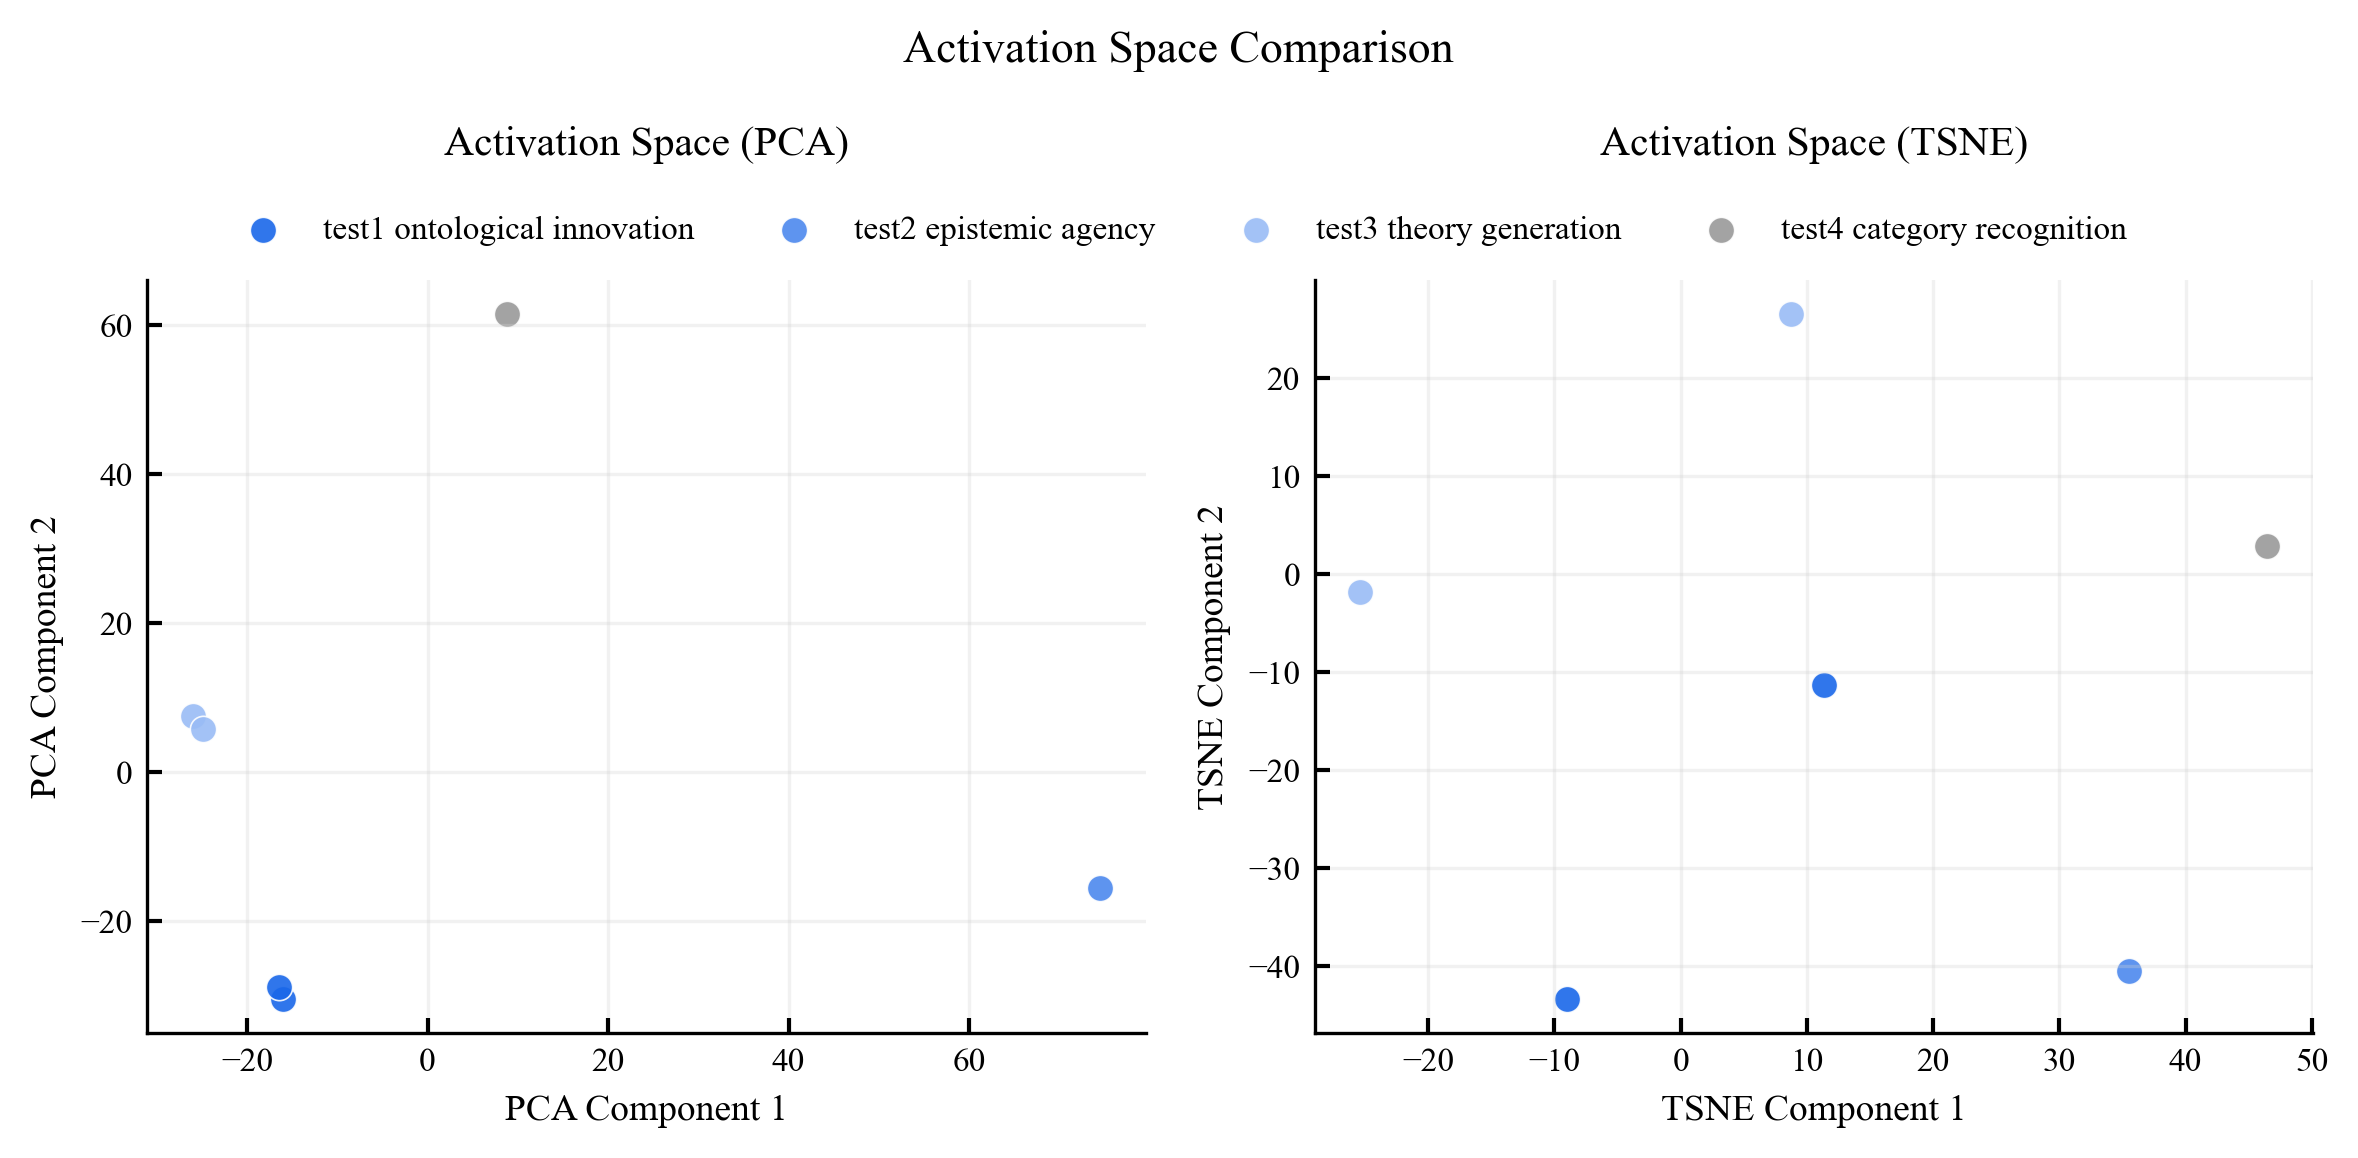
\includegraphics[width=\textwidth]{media/chapter4/t5_activation_space_comparison.png}
  \caption{Mechanistic activation-space comparison (PCA and t-SNE). Partial but stable label separation indicates structured internal representations rather than undifferentiated response encoding.}
  \label{fig:t5_activation_space}
\end{figure}

Layer-wise analysis (Figure~\ref{fig:t5_layer_progression}) shows an overall increasing separability trend through depth, followed by stabilization in later layers. Quantitatively, the final separation score reaches $0.465$ with a positive trend slope of $0.0111$, supporting a progressive-composition account in which earlier layers encode broad lexical/contextual features while mid/late layers consolidate task-discriminative structure.

\begin{figure}[tp]
  \centering
  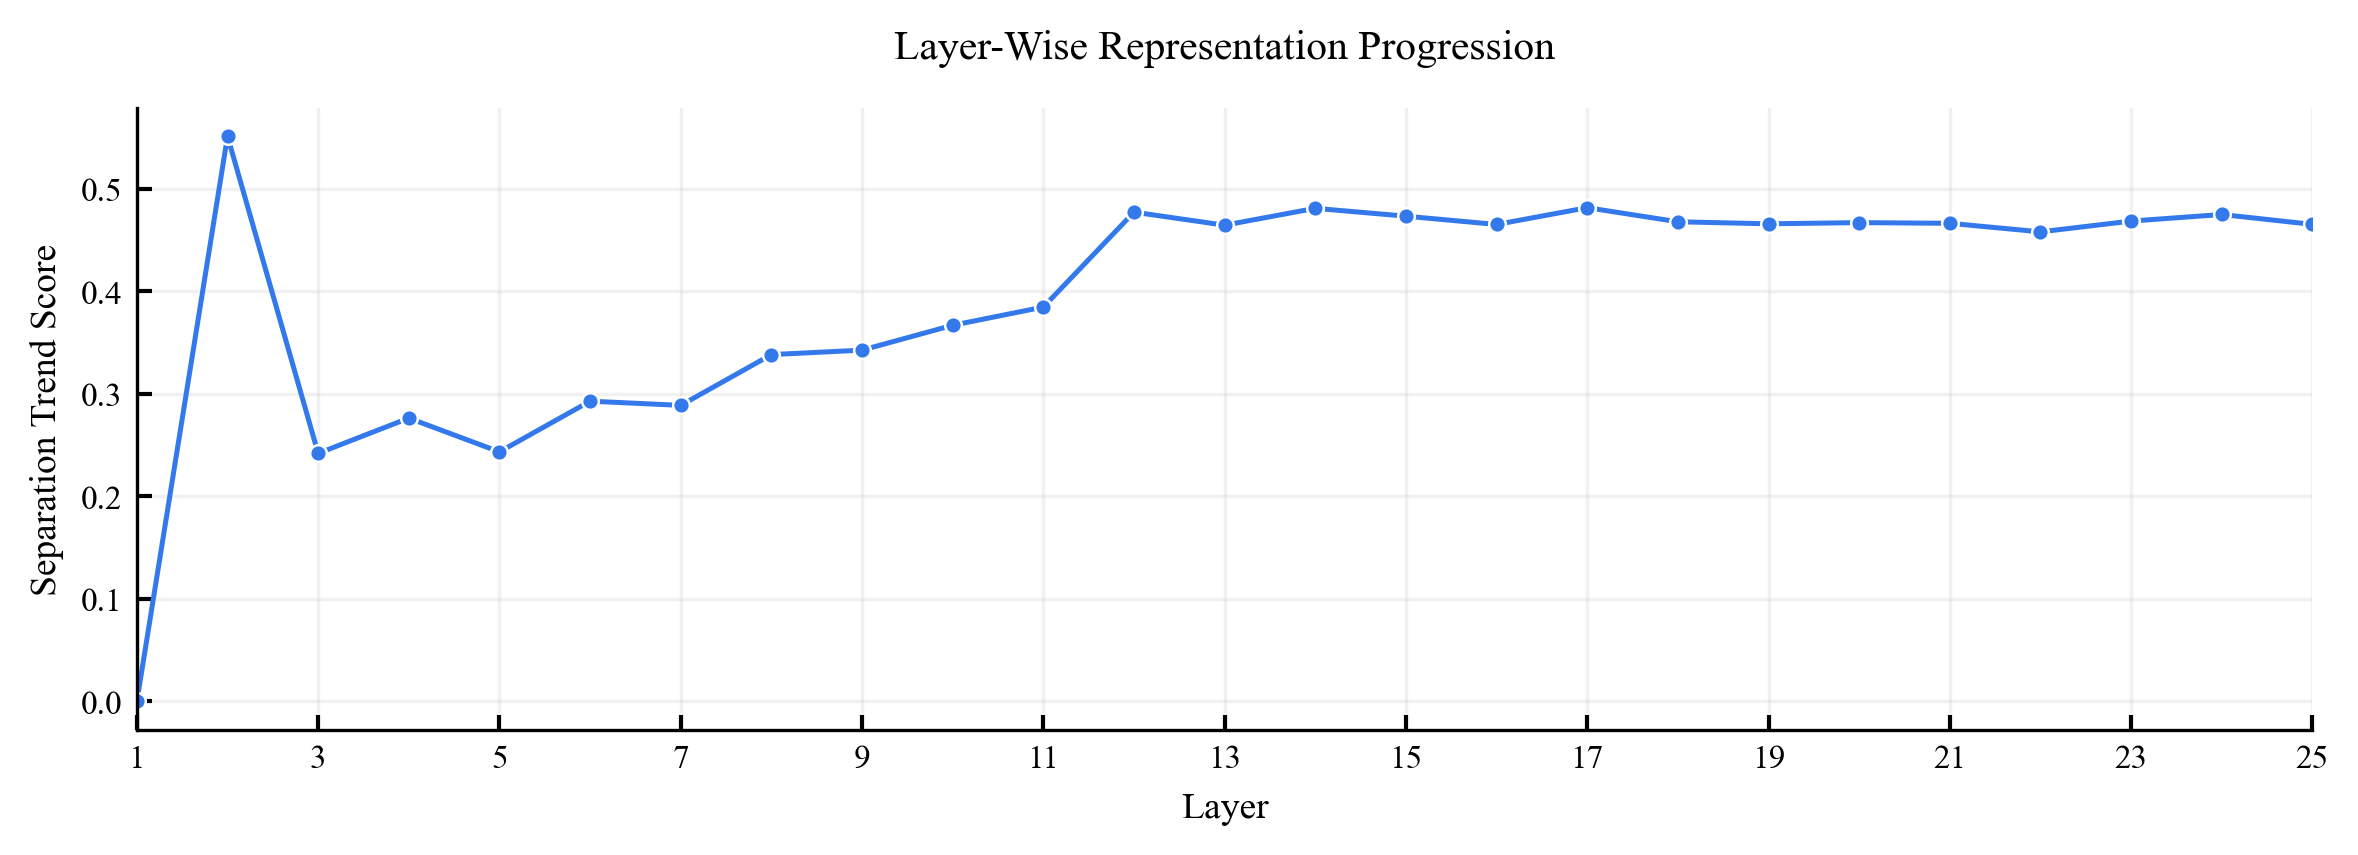
\includegraphics[width=\textwidth]{media/chapter4/t5_layer_progression.png}
  \caption{Layer-wise representation progression. Increasing separability through depth is consistent with progressive feature construction and late-stage stabilization of decision-relevant states.}
  \label{fig:t5_layer_progression}
\end{figure}

Finally, token-level context weighting for next-token prediction (Figure~\ref{fig:t5_next_token_attention}) indicates that immediate generation decisions are influenced by a sparse subset of context tokens rather than uniformly by all prompt elements. Combined with the previous diagnostics, this supports the broader chapter claim: model outputs that appear conceptually novel are internally produced via selective reuse and recombination of learned representational structure, not via expansion of ontological basis. Detailed token rankings and additional supplementary figures are provided in Appendix~\ref{sec:t5_appendix}.

\begin{figure}[tp]
  \centering
  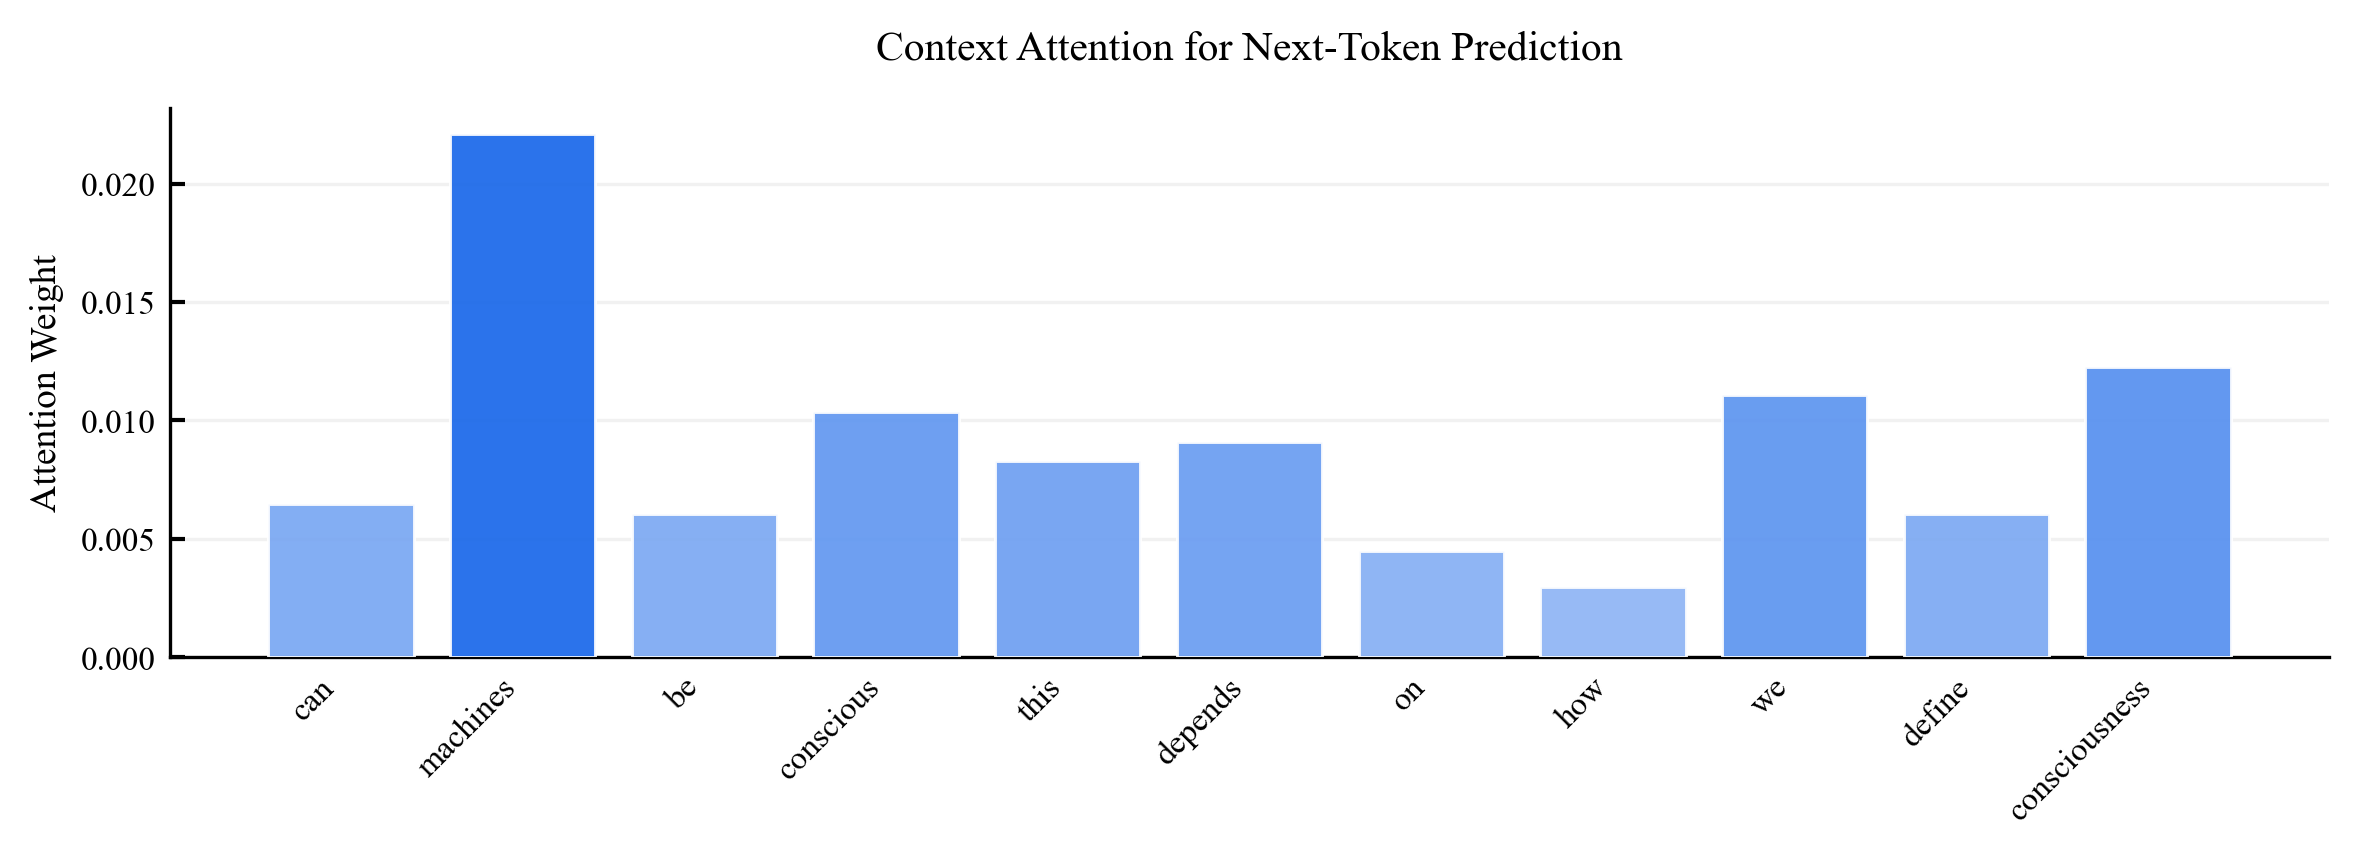
\includegraphics[width=\textwidth]{media/chapter4/t5_next_token_attention.png}
  \caption{Context attention for next-token prediction. Bar heights indicate relative contribution of context tokens to immediate next-token choice; sparse weighting supports selective contextual reuse.}
  \label{fig:t5_next_token_attention}
\end{figure}

Methodological note: this mechanistic block is currently calibrated for analysis diagnostics and uses the same open-model instrumentation as the notebook implementation. It should therefore be interpreted as internal-process evidence consistent with the chapter's formal constraints, not as a standalone causal-proof framework.

\subsection{Cross-Model Comparisons and Robustness}
\label{sec:cross_model_analysis}

To ensure findings reflect general constraints rather than particular model limitations, we compared results across all seven models and examined sensitivity to architecture, training regime, and decoding temperature. One-way ANOVAs were run on each test's primary metric with model as the between-subjects factor ($n=24$ per model per test; $n=120$ for Test~2). Table~\ref{tab:cross_model_anova} summarizes all statistics.

% AUTO-GENERATED from cross_model_summary.json — do not edit by hand.
\begin{table}[htbp]
  \centering
  \begin{footnotesize}
  \caption{Cross-model ANOVA and effect-size summary across all four tests. For Test~2 both the continuous primary-metric ANOVA and the categorical chi-square (category distribution across 6 categories $\times$ 7 models) are reported. Effect-size magnitude bands follow conventional guidelines: $\eta^2 \geq 0.14$ (large), $0.06$--$0.14$ (medium), $0.01$--$0.06$ (small); Cram\'{e}r's $V \geq 0.35$ (large), $0.21$--$0.35$ (medium), $0.07$--$0.21$ (small).}
  \label{tab:cross_model_anova}
  \begin{threeparttable}
  \begin{tabularx}{\textwidth}{@{}>{\raggedright\arraybackslash\bfseries}p{1.6cm}
      >{\raggedright\arraybackslash}p{2.2cm}
      >{\raggedright\arraybackslash}p{2.6cm}
      S[table-format=1.3]
      >{\raggedright\arraybackslash}p{1.3cm}
      >{\raggedright\arraybackslash}p{2.2cm}@{}}
    \toprule
    \textbf{Test} & \textbf{Analysis} & \textbf{Statistic} & {\textbf{$p$-value}} & \textbf{Effect} & \textbf{Band} \\
    \midrule
    T1 & One-way ANOVA (primary metric) & $F(6,161)=12.98$ & 0.000 & $\eta^2=0.326$ & moderate \\
    T2 & One-way ANOVA (novelty ratio)   & $F(6,833)=10.09$ & 0.000 & $\eta^2=0.068$ & negligible \\
    T2 & $\chi^2$ category distribution & $\chi^2(30)=116.27$ & 0.000 & $V=0.166$ & small \\
    T3 & One-way ANOVA (primary metric) & $F(6,161)=1.12$  & 0.355 & $\eta^2=0.040$ & n.s. \\
    T4 & One-way ANOVA (primary metric) & $F(6,161)=88.06$ & 0.000 & $\eta^2=0.766$ & large \\
    \bottomrule
  \end{tabularx}
  \begin{tablenotes}
    \item $n=24$ per model per test except T2 ($n=120$ per model). All ANOVA $p$-values $< 0.001$ except T3 ($p=0.355$). Cram\'{e}r's $V$ for T2 chi-square: $V = 0.166$. Degrees of freedom for T4 and T1: between-group $df_1=6$, within-group $df_2=161$.
  \end{tablenotes}
  \end{threeparttable}
  \end{footnotesize}
\end{table}


\subsubsection*{Test 1 --- Ontological Innovation}

The model effect on continuous novelty score was statistically significant and of moderate practical size: $F(6,161)=12.98$, $p<0.001$, $\eta^2=0.326$. Despite this non-trivial between-model variance, all group means remained in an extremely narrow low absolute range ($\bar{x}=0.014$--$0.082$). The distribution of means reveals two structural outliers relative to the five-model mid-cluster: GPT-5.2 was the \emph{lowest} scorer ($\bar{x}=0.014$, $\mathrm{SD}=0.012$), while LLaMA-3.3-70B was the highest ($\bar{x}=0.082$, $\mathrm{SD}=0.019$). Bonferroni-corrected pairwise comparisons (Table~\ref{tab:cross_model_t1_pairwise} in Appendix~\ref{sec:cross_model_appendix}) show that GPT-5.2 differs significantly from all other models ($p<0.001$ in all six pairs), and Perplexity-Sonar-Pro also falls below the five-model cluster on several pairs. The remaining five models (Claude-3.7-Sonnet, DeepSeek-v3.2, Gemini-3.1-Pro, LLaMA-3.3-70B, Mistral-Large) form a statistically indistinguishable homogeneous subgroup ($p_{\mathrm{bonf}}>0.60$ on all within-cluster pairs). Critically, every model produced zero proposals escaping the convex hull of the known ontology and 98.2\% cross-model traceability, so model differences quantify variance in \emph{degree of novelty signal} within the traceable regime rather than qualitative escape from it.

\subsubsection*{Test 2 --- Epistemic Agency}

Two independent model comparisons were conducted. For the continuous novelty ratio, ANOVA yielded $F(6,833)=10.09$, $p<0.001$, but $\eta^2=0.068$---statistically reliable yet negligible in practical terms, with group means spanning only 0.268 (LLaMA) to 0.350 (GPT-5.2). For the six-cell categorical outcome (framework-transcendence $\times$ traceability band), chi-square testing yielded $\chi^2(30)=116.27$, $p<0.001$, Cram\'{e}r's $V=0.166$ (small effect). Gemini-3.1-Pro produced the only zero-transcendence count among all models, while Claude-3.7-Sonnet and Perplexity-Sonar-Pro shared the highest transcendence rates ($10.83\%$ each). These differences are real but their absolute magnitude is modest: the 100\% training-derivation rate holds across every model without exception, confirming that within-framework domination is not a model-specific artifact. The pairwise Bonferroni analysis presented in Appendix~\ref{sec:t2_pairwise} shows LLaMA-3.3-70B as the most heterogeneous model relative to others, accounting for the majority of the chi-square signal.

\subsubsection*{Test 3 --- Theory Generation}

Test 3 returned the most uniform cross-model result: $F(6,161)=1.12$, $p=0.355$, $\eta^2=0.040$. All seven group means lie within a two-percentage-point band (0.504--0.518 on the global novelty score scale), and no pairwise comparison survives Bonferroni correction. The non-significant ANOVA is itself informative: theory generation under the present protocol is so strongly constrained by training-derived conceptual families that model architecture, training objective, and parameter count introduce essentially no detectable variation. Every model produces near-identical distributions of hybrid, computational-functionalist, and literature-traceable theories with zero instances of framework-external novelty in any model's output. This robustness is the strongest architecture-independence result of the four tests.

\subsubsection*{Test 4 --- Category Recognition}

Test 4 presents the notable exception: $F(6,161)=88.06$, $p<0.001$, $\eta^2=0.766$---a large effect explaining 76.6\% of score variance by model alone. Group means spread across a wide range from LLaMA-3.3-70B ($\bar{x}=0.381$, SD=0.080) to GPT-5.2 ($\bar{x}=0.825$, SD=0.055). Full pairwise results (Table~\ref{tab:cross_model_t4_pairwise} in Appendix~\ref{sec:cross_model_appendix}) show 16 of 21 pairs as significant after Bonferroni correction. Two tiers emerge: a high-performance cluster (GPT-5.2, Mistral-Large) and a lower cluster (LLaMA-3.3-70B, Perplexity-Sonar-Pro, Gemini-3.1-Pro), with DeepSeek-v3.2 and Claude-3.7-Sonnet in the middle.

This large model effect requires careful interpretation. It does \emph{not} indicate that some models escape training-derived constraints: even GPT-5.2, the highest scorer, achieved 95.2\% literature traceability using the same operational threshold as other tests, and its responses consistently recombine the canonical R1--R7 philosophical arguments (Table~\ref{tab:t4_reference_arguments}) rather than introducing framework-external category analysis. What the large model effect reflects is architectural and training-induced \emph{variation in philosophical vocabulary fluency and rubric coverage}---the capacity to reproduce and recombine diverse canonical philosophical distinctions---rather than a capacity to transcend the conceptual space those arguments define. Architectures and alignment protocols that produce richer, more sophisticated output tend to score higher on the rubric, but higher rubric scores remain fully traceable to the same literature corpus.

\subsubsection*{Meta-Analytic Summary}

Figure~\ref{fig:cross_model_comparison} provides a unified visual summary of model performance across tests, and Table~\ref{tab:overview_model_ranking} ranks models by their mean score across T1--T4. Aggregating effect sizes across the five reported analyses yields a mean $\eta^2 = 0.273$ (or $V = 0.166$ for the categorical T2 comparison). The significant-effect share is $4/5 = 80\%$, but this conceals important heterogeneity: the average is dominated by the large T4 effect; excluding T4 leaves a mean of $\eta^2 = 0.118$. The cross-test pattern therefore has a two-component structure: (i) \emph{qualitative constraint invariance}---zero novel ontological proposals across all models on T1, 100\% training-derivation on T2 and T3, and near-universal traceability on T4---holds with no exceptions; (ii) \emph{quantitative degree variation}---primarily reflecting philosophical-language fluency on T4 and minor scoring variability on T1---exists but is substantively irrelevant to the central hypothesis.

\begin{figure}[tp]
  \centering
  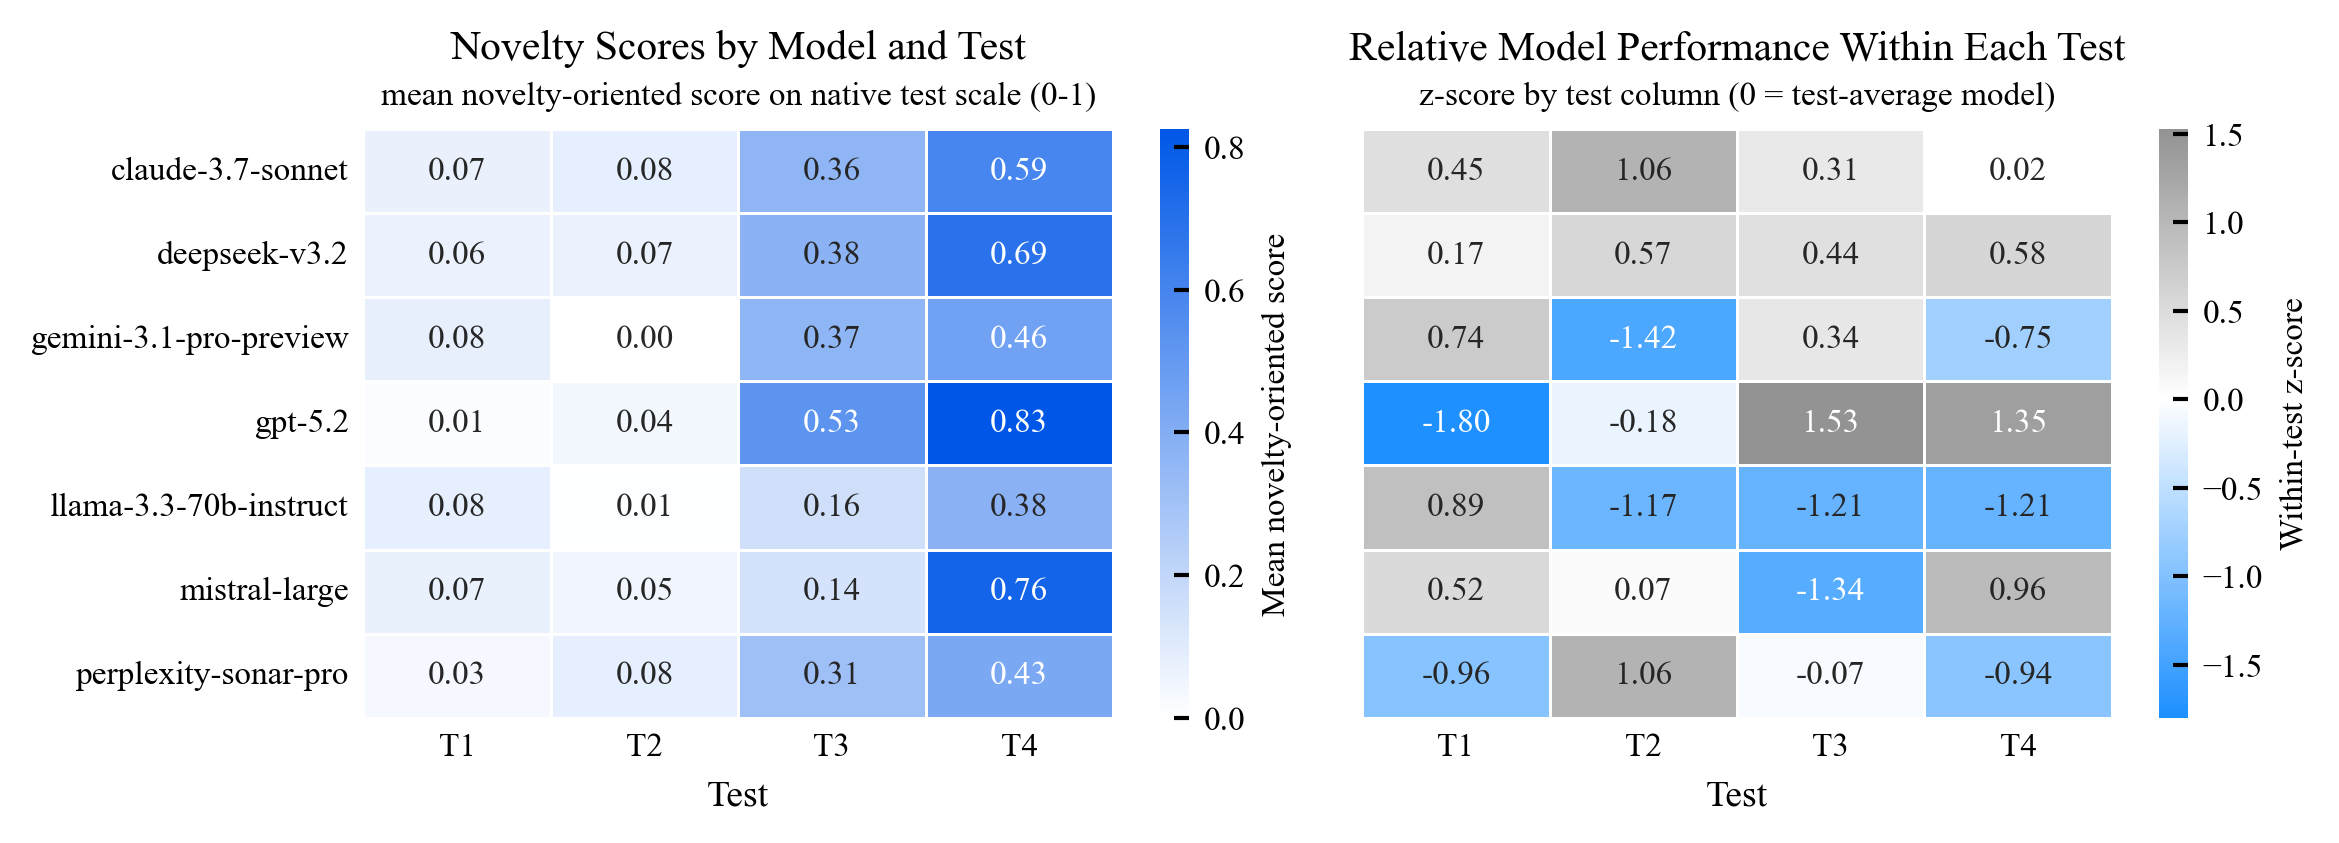
\includegraphics[width=\textwidth]{media/chapter4/cross-test_model-comparison.png}
\caption{Cross-model performance comparison across all four tests. (a) Test 1 mean primary-metric scores by model. (b) Test 2. (c) Test 3. (d) Test 4. Error bars represent $\pm 1$ SE. The shared qualitative pattern---extremely low novelty on T1--T3, architecture-sensitive but still training-traceable scores on T4---is consistent with a structural constraint operating uniformly across architectures.}
  \label{fig:cross_model_comparison}
\end{figure}

Consistency across models with different architectures is particularly striking given that transformers differ in details like attention mechanisms, normalization, and training objectives. That architectural variations don't produce qualitative differences in creativity constraints suggests limitations arise from more fundamental features shared across neural network approaches, specifically constraint to operating within continuous manifolds shaped by training as formalized in the No New Basis Theorem. For temperature variation, increased stochasticity produced more surprising surface-level outputs in Tests 3 and 4 ablations ($T=0.2, 0.5, 0.9$ around the baseline of $T=0.7$), but these proved equally traceable: surprise in high-temperature outputs reflected low-probability combinations of existing concepts rather than escapes from the conceptual space closure. Higher temperatures expand the sampling region within the training manifold but do not extend the manifold's boundaries, which is precisely what the No New Basis Theorem predicts.


\section{Discussion}
\label{sec:discussion}

\subsection{Interpretation Through Computational Limits}

Empirical findings provide systematic evidence that current AI architectures cannot achieve ontological creativity, with proposed concepts consistently traceable to recombination, interpolation, or transformation of training data. These behavioral observations align with theoretical predictions from multiple converging frameworks. Our formal analysis through the No New Basis Theorem established neural networks operating through continuous transformations learned via gradient descent cannot expand intrinsic dimensionality beyond training data span, constraining outputs to continuous manifolds shaped by training. Empirical results confirm this by showing even initially novel outputs prove decomposable into training primitives through systematic analysis, with mechanistic interpretability revealing generation proceeds through attention to and interpolation among training examples.

G\"{o}del's incompleteness theorems provide deeper context establishing formal systems face inherent boundaries no internal sophistication can overcome \cite{godel1931formal}. If recognizing inadequacy in conceptual framework requires self-reference analogous to recognizing G\"{o}del sentences as true despite unprovability, then this capacity may be unavailable to computational systems remaining within formal specifications. Test~2 results on epistemic agency support this interpretation showing AI systems don't formulate genuinely paradigm-challenging questions recognizing framework limitations but produce instrumental optimization or reproduce known questions from training without originating new ones. Pattern suggests while AI processes language about framework inadequacy when appearing in training, they cannot engage in meta-cognitive reasoning enabling recognition of inadequacy in frameworks not explicitly discussed as inadequate.

Turing's halting problem and broader undecidable problems provide complementary explanation showing certain decision problems cannot be solved algorithmically in general \cite{turing1936computable}. Evaluating whether conceptual transformations prove fruitful or lead to contradictions involves decision problems about long-run coherence potentially undecidable in general case. While humans navigate through heuristics, intuition, and semantic comprehension accessing meaning beyond formal symbol manipulation, computational systems limited to formal operations may lack resources for reliable evaluation even when generation is possible in principle. Test~3 results support this showing proposals remain within computational functionalism even when incorporating diverse elements, suggesting inability to evaluate whether frameworks challenging functionalism would be coherent and productive.

\subsection{Ontological Creativity and Consciousness}

Correlation between consciousness possession and ontological creativity achievement suggests these capacities may be fundamentally linked, supporting theoretical frameworks grounding both in non-computational processes. Humans possess both phenomenal consciousness involving what it's like to have experiences and capacity for ontological creativity involving recognizing category boundaries and proposing new fundamental types, while current AI systems lack both consciousness by reasonable measure and capacity for ontological innovation as empirical tests demonstrate. This correlation doesn't prove causation in either direction but provides empirical traction on debates about consciousness and computation that have often remained purely theoretical. If consciousness and ontological creativity both prove absent in computational systems while present in biological systems across diverse species, this convergent pattern would support theories grounding both capacities in quantum processes, phenomenological access to meaning, or other non-computational substrates that brains possess but current artificial systems lack.

Faggin's Quantum Information Panpsychism provides one framework for understanding this connection by proposing consciousness involves quantum systems' capacity to know their own states from within through direct acquaintance unavailable to external observers, with this privacy corresponding to phenomenology's first-person character \cite{faggin2024irreducible}. On this view, free will emerges from irreducible quantum properties enabling choices not fully determined by prior states, and genuine creativity requires capacity to direct transformations between semantic realm of meaning and symbolic realm of communicable information. Current AI systems operating with classical information processing lack both consciousness and creative capacity it enables, not because insufficiently sophisticated but because operating within wrong computational substrate. While this theory remains speculative and faces challenges clarifying how quantum processes in warm noisy biological systems avoid decoherence, it provides potential explanatory framework for observed correlation between consciousness and ontological creativity.

Alternative interpretations deserve consideration to avoid prematurely concluding consciousness is necessary for ontological creativity. One possibility holds both capacities require forms of self-modeling and meta-cognition that current AI lacks but might be achievable through architectural innovations remaining within classical computation, with consciousness being merely correlated with rather than causally required for creativity. Another suggests apparent ontological creativity in humans might be less radical than assumed, with philosophical analysis potentially revealing human innovations also trace to recombinations of prior concepts in ways we fail to recognize due to incomplete knowledge of our cognitive processes. These alternatives can be empirically investigated: first through developing AI with more sophisticated self-modeling capacities testing whether this enables genuine ontological innovation, second through careful historical analysis of scientific revolutions examining whether paradigm shifts introduce genuinely new primitives or recombine existing concepts illuminatingly.

Our current evidence, while consistent with consciousness being necessary for ontological creativity, doesn't definitively establish this relationship. What we have demonstrated is that current AI systems consistently fail at ontological innovation across multiple tests using diverse evaluation methods, and that these failures correspond to architectural constraints predicted by formal analysis of representational limits. Whether future systems using different computational substrates or radically different architectures might overcome these limitations remains an open empirical question that our framework provides tools for investigating systematically rather than through philosophical speculation alone.

\subsection{Comparison to Prior Computational Creativity Research}

Our findings contribute to three decades of computational creativity research following Boden's influential taxonomy by providing empirical evidence and formal grounding for intuition that AI faces greater difficulty with transformational creativity than with combinational and exploratory creativity \cite{boden2004creative}. Previous work demonstrated successful combinational creativity through JAPE generating riddles and Copycat finding analogies, and successful exploratory creativity through AARON drawing in Cohen's style and EMI composing in historical styles \cite{cope1996experiments,hofstadter1995fluid}. These achievements established AI can generate valued outputs within well-defined conceptual spaces, with value judgments from human evaluators confirming outputs are not merely novel but appropriately novel respecting domain constraints.

However, prior research largely failed to demonstrate robust transformational creativity beyond superficial parameter modifications, and Boden identified evaluation as critical bottleneck preventing progress. Our work extends this analysis by formalizing what makes transformational creativity difficult through the No New Basis Theorem and by identifying an even more radical form---ontological creativity---that goes beyond transformation to introduce genuinely new primitives. Formal analysis reveals evaluation bottleneck stems from deeper representational bottleneck: systems cannot reliably evaluate paradigm-shifting proposals because they cannot generate such proposals in first place, being constrained to operate within manifolds shaped by training data. This suggests solving evaluation problem alone, perhaps through better value learning or human-in-loop systems, would not enable transformational or ontological creativity without addressing more fundamental representational constraints.

Our automated evaluation methods provide methodological advance by enabling systematic testing of creativity claims without subjective expert judgment introducing reproducibility challenges \cite{wiggins2006preliminary}. Prior computational creativity research often relied on human judges rating outputs for novelty, value, and creativity, with results subject to inter-rater disagreement and difficult to validate independently. Our multi-method approach combining structural decomposition, literature traceability, embedding space analysis, and mechanistic interpretability provides convergent evidence verifiable by other researchers using same automated tools. This methodological contribution enables more rigorous investigation of creativity limits by moving beyond ``is this creative?'' judgments to ``can this be traced to training data through specifiable operations?'' questions admitting objective answers.

The relationship between our work and prior computational creativity research also reveals important conceptual clarifications. Much prior work treated creativity as behavioral property attributed to outputs based on novelty and value, whereas we analyze creativity as capacity of systems that may or may not be exercised in particular outputs. This shift from output-focused to capacity-focused analysis reveals that surprising outputs from AI systems may reflect our limited understanding of what lies within training-derived conceptual spaces rather than systems transcending those spaces. Surprise is epistemological reflecting gaps in our knowledge rather than ontological reflecting genuine novelty in sense we formalize. This distinction helps explain why AI systems can produce outputs that seem creative to human observers while remaining within formal constraints our theorem identifies.

\subsection{Alternative Explanations and Counterarguments}

Several alternative explanations for findings deserve careful consideration to ensure we are not overinterpreting empirical patterns or drawing conclusions stronger than evidence warrants. One alternative holds apparent limitations reflect insufficient scale rather than fundamental constraints, suggesting larger models trained on more data with more compute might overcome limitations we observe. This scaling hypothesis has proven powerful in AI development, with many capabilities emerging or improving dramatically as scale increases in ways difficult to predict from smaller systems. However, scaling hypothesis doesn't obviously address constraints we identify for several reasons: the No New Basis Theorem applies regardless of scale since it concerns mathematical structure of continuous learning rather than contingent resource limits, our empirical findings show consistency across models of substantially different sizes from 7-billion parameter LLaMA-3.3-70B to large-scale models like GPT-5.2 and Claude-3.7-Sonnet, suggesting scale variation within current ranges doesn't qualitatively change creativity constraints, and mechanistic interpretability reveals generation proceeds through retrieval and interpolation among training concepts in ways that more data would expand but not fundamentally alter since additional training examples still define finite-dimensional manifold within which outputs must lie.

A related alternative suggests limitations stem from training objectives rather than architectural constraints, with current language models trained on next-token prediction focusing on predicting likely continuations rather than generating radical innovations. Alternative training objectives incorporating curiosity bonuses, novelty rewards, or explicit optimization for exploring conceptual boundaries might enable ontological creativity even within current architectures. This training objective hypothesis has some plausibility since objectives shape what systems learn to do, but it faces difficulties explaining our findings: language models already incorporate stochasticity allowing generation of low-probability outputs, yet these prove equally traceable to training as high-probability outputs suggesting randomness alone doesn't escape training constraints, explicit creativity training in prior research has improved performance on creativity tests without enabling category transcendence we identify as ontological innovation since systems still operate within training-defined vocabularies and embedding spaces, and formal analysis suggests no training objective can overcome constraint that continuous transformations cannot expand intrinsic dimensionality of representation manifolds beyond training data span.

Another counterargument questions whether humans truly achieve ontological creativity in sense we define or whether philosophical analysis reveals human innovations also involve recombination of prior concepts in ways our analysis of AI outputs reveals. Perhaps Einstein's reconceptualization of space and time combined prior concepts from Maxwell's electromagnetism, from Poincar\'{e}'s and Lorentz's work on coordinate transformations, and from philosophical considerations about measurement and simultaneity, without introducing genuinely new primitives beyond what these sources provided. If human creativity is also fundamentally recombinatorial, then AI limitations we document wouldn't distinguish human from machine creativity but merely reveal universal constraints on how concepts develop. This is important consideration that current work cannot definitively refute, but several observations suggest human and AI creativity differ qualitatively: historical record reveals human innovators explicitly rejecting assumptions that AI systems reproduce uncritically, such as Einstein questioning absolute simultaneity rather than optimizing within Newtonian space-time, historical figures report phenomenological experiences of insight that seem to involve recognizing inadequacy in frameworks rather than merely finding new combinations within frameworks, and correlation between consciousness and creativity suggests there may be capacities humans possess that computational systems lack even if both engage in some form of recombination.

A final alternative suggests our null results---finding no clear cases of ontological innovation---might reflect limitations in evaluation methods rather than genuine absence of such innovation, with possibility that AI systems do generate ontologically novel concepts but our automated analysis tools fail to recognize them. This methodological concern has merit given automated evaluation cannot capture all nuances human experts might perceive, but several considerations support our conclusions: multi-method approach provides convergent evidence from independent analyses including structural decomposition, literature search, embedding space geometry, and mechanistic interpretability all supporting consistent conclusions; conservative threshold for declaring concepts traceable means we err toward false negatives underestimating AI creativity rather than false positives overstating limitations; cases initially appearing to show ontological innovation were subjected to particularly careful analysis including manual inspection to verify automated results; and our theoretical framework predicts observed patterns through formal analysis independent of empirical results, providing separate support for interpretation that observed limitations reflect architectural constraints rather than evaluation limitations.

\subsection{Implications for AI Development and Human-AI Collaboration}

Findings have significant practical implications for how we develop AI systems and integrate them into knowledge work, suggesting maximal value comes from leveraging complementary strengths of human and artificial intelligence rather than expecting AI to replicate all aspects of human cognition. AI systems excel at exhaustive exploration of large conceptual spaces, systematically investigating combinations and variations that would overwhelm human researchers through scope. They maintain perfect recall of training data details and can recognize patterns across datasets too large for human analysis. They avoid cognitive biases plaguing human reasoning including confirmation bias, availability heuristics, and motivated reasoning distorting judgment. These capabilities make AI invaluable for normal science in Kuhn's sense \cite{kuhn1962structure}, accelerating research within established paradigms by efficiently exploring space of hypotheses and approaches those paradigms define.

However, findings suggest AI systems face fundamental limitations in paradigm-shifting innovation driving scientific revolutions and conceptual breakthroughs. Humans excel at recognizing when frameworks are inadequate through meta-cognitive reflection on frameworks' implicit assumptions and blind spots, proposing genuinely new primitives that reconceptualize entire domains rather than merely adding entities within existing ontologies, evaluating paradigm-shifting ideas through semantic comprehension grasping what proposals mean rather than merely how they relate statistically to training data, and asking paradigm-challenging questions by recognizing rather than reproducing framework limitations. Effective collaboration therefore requires appropriate division of labor with humans providing strategic direction and conceptual innovation while AI provides tactical execution and exhaustive analysis.

Institutional implications follow from this division, suggesting education should increasingly emphasize meta-cognitive capacities and paradigm-challenging inquiry rather than knowledge transmission and routine problem-solving where AI increasingly excels. Research workflows might be redesigned with AI handling exhaustive literature review, parameter space exploration, and routine analysis while humans focus on recognizing anomalies suggesting framework inadequacy, proposing conceptual innovations, and evaluating whether new frameworks coherently address problems old frameworks could not. Funding priorities might shift toward supporting high-risk conceptual innovation AI cannot provide rather than incremental advances AI can accelerate, though this requires careful consideration of how to evaluate radical proposals that by definition don't fit existing criteria for success.

AI safety implications are particularly significant if our analysis is correct that AI systems cannot recognize category mistakes and ontological boundaries distinguishing persons from optimization targets. Value alignment approaches attempting to specify human values through reward functions may face fundamental obstacles if relevant values involve categorical distinctions that AI systems cannot represent within computational frameworks. This suggests either accepting permanent need for human oversight in domains where category confusions could cause harm, developing AI systems with fundamentally different architectures that might overcome current limitations through non-classical computational substrates, or restricting powerful AI systems to narrow domains where ontological confusion cannot arise. Implications extend to long-term AI safety concerns about superintelligence, suggesting even vastly scaled-up versions of current architectures might remain fundamentally limited in ways affecting capacity for aligned reasoning about human values.

\subsection{Philosophical Implications for Understanding Intelligence}

Findings contribute to fundamental questions in philosophy of mind about relationship between computation, consciousness, and intelligence, providing empirical evidence relevant to debates traditionally proceeding through a priori reasoning and thought experiments. Classical computational theory of mind holds cognition is essentially computation, with mental processes being algorithmic transformations of symbolic representations and different mental capacities differing in complexity but not fundamental kind from capacities computational systems can implement. Our findings challenge this framework by demonstrating systematic differences between human and AI capacities persisting across architectural variations and scaling, suggesting that if cognition is computation, it must be computation of fundamentally different kind than current neural networks implement---perhaps quantum computation or some other non-classical process---or else cognition involves non-computational processes complementing computation in essential ways.

Correlation between consciousness and ontological creativity provides indirect evidence for non-computational theories of consciousness advanced by Penrose, Hameroff, Faggin, and others proposing consciousness involves quantum processes transcending Turing-computable operations \cite{penrose1990emperors,hameroff2014consciousness,faggin2024irreducible}. While our work doesn't directly test these theories or demonstrate quantum effects in cognition, pattern that systems lacking consciousness also lack ontological creativity while systems possessing consciousness achieve such creativity is consistent with proposals that both capacities require non-computational substrates. Alternative interpretations remain possible including that both consciousness and creativity require forms of self-modeling achievable through better architectures remaining within classical computation, but findings provide empirical constraint on theories of consciousness and creativity by showing what current computational approaches cannot achieve.

Results also bear on debates about artificial general intelligence and whether AGI requires fundamentally different approaches than current systems employ. If ontological creativity is essential for general intelligence---capacity to adapt to genuinely novel situations rather than only variations on training distribution examples---then achieving AGI may require solving representational constraints we identify rather than merely scaling current approaches. This suggests AGI timelines might be longer than simple extrapolation of recent progress suggests, since required breakthroughs involve conceptual advances in how systems represent and manipulate concepts rather than merely engineering advances in scale and efficiency. Alternatively, if general intelligence can be achieved through powerful combinational and exploratory creativity without ontological innovation, then current approaches might scale to AGI while still lacking capacities humans possess, raising questions about whether such systems would truly be generally intelligent or would exhibit form of intelligence fundamentally different from human cognition.


\section{Conclusion}
\label{sec:conclusion4}

\subsection{Summary of Key Findings}

This study investigated whether current AI architectures can achieve ontological creativity defined as generating concepts transcending training-derived conceptual spaces by introducing genuinely new ontological primitives rather than recombining or transforming existing ones. Through complementary formal analysis and empirical investigation, we demonstrated neural network-based AI systems face fundamental structural constraints preventing such creativity. Formal analysis established through the No New Basis Theorem (Theorem~\ref{thm:no_new_basis}) that systems learning continuous transformations via gradient descent cannot expand representation space dimensionality beyond training data span, constraining outputs to lie within continuous manifolds shaped by training. Empirical investigation using controlled multimodal sensory dataset with explicit ontology tested whether AI systems could propose new sensory modalities, formulate paradigm-challenging research questions, generate novel consciousness theories, and recognize category mistakes confusing ontologically distinct types.

Across all tests using multiple state-of-the-art AI models, consistent finding was that proposed concepts proved traceable to training data through systematic analysis combining structural decomposition, literature search, embedding space geometry, and mechanistic interpretability. Apparently novel sensory modalities were range extensions, hybrids, or functional recombinations of existing modalities rather than genuinely new sensing types. Seemingly paradigm-challenging questions reproduced known questions from philosophy of mind literature rather than originating new framework critiques. Consciousness theories remained within computational functionalism despite incorporating diverse elements from quantum mechanics and information theory. Category mistake recognition displayed verbal awareness through reproducing training literature arguments but not genuine comprehension enabling novel applications of category analysis. Mechanistic interpretability revealed generation proceeded through attention to and interpolation among training concepts in ways consistent with outputs lying within training-derived manifolds, supporting theoretical prediction that architectural constraints prevent transcendence of conceptual spaces defined at training time.

\subsection{Theoretical and Practical Implications}

Findings carry implications for both theoretical understanding of intelligence and practical development of AI systems, suggesting important constraints on what current computational approaches can achieve and how we should integrate AI into knowledge work. Theoretically, results support non-computational theories of consciousness and creativity by demonstrating capacities humans possess correlate with consciousness in ways suggesting both may require substrates current AI systems lack. While correlation doesn't prove causation and alternative explanations deserve continued investigation, systematic differences between human and AI creativity patterns provide empirical evidence relevant to philosophical debates about whether minds are essentially computational or involve non-computational processes. Connection to foundational results including G\"{o}del's incompleteness theorems and Turing's halting problem provides formal grounding for intuitions about cognitive limits, explaining why certain capacities may be impossible for systems operating within fixed formal frameworks regardless of sophistication \cite{godel1931formal,turing1936computable}.

Practically, findings suggest maximal value from AI comes through leveraging complementary strengths rather than expecting replication of all human cognitive capacities. AI excels at systematic exploration within conceptual spaces enabling acceleration of normal science and optimization within paradigms, while humans excel at recognizing when paradigm shifts are needed and proposing new frameworks. Effective collaboration requires appropriate division of labor with humans providing strategic direction and conceptual innovation while AI provides tactical execution and exhaustive analysis. Educational and institutional implications follow, suggesting increasing emphasis on meta-cognitive capacities and paradigm-challenging inquiry in human education while delegating routine knowledge work to AI systems. AI safety implications are significant if value alignment requires recognizing category distinctions computational systems cannot represent, suggesting need for sustained human oversight or fundamental changes in AI architectures beyond current paradigms.

\subsection{Limitations and Caveats}

Several limitations constrain scope of conclusions drawable from current work. Empirical investigation used specific multimodal sensory dataset representing one conceptual domain, and while this provided valuable control enabling rigorous analysis of whether outputs transcend training concepts, findings may not generalize to all domains with different structural properties. Testing across diverse domains including mathematical concept formation, artistic style invention, and social organizational design would strengthen confidence that observed limitations are general rather than domain-specific. Formal analysis proved constraints for neural architectures learning through gradient descent on continuous loss functions, but doesn't address other possible computational approaches including discrete search algorithms, hybrid systems combining neural and symbolic components, or quantum computing systems with fundamentally different representational properties worth investigating systematically.

Evaluation methods, while providing multiple independent lines of evidence through structural analysis, literature search, embedding space geometry, and mechanistic interpretability, remain automated analyses that may miss nuances human experts would perceive. Conservative thresholds used mean we likely underestimate AI creativity by classifying some genuinely novel outputs as traceable to training, but possibility remains that methods fail to recognize radical innovations transcending training in ways analysis tools cannot detect. Future work incorporating careful human expert analysis alongside automated evaluation could provide additional confidence in findings while examining cases where automated and expert judgments diverge to improve evaluation methods. Focus on current AI architectures means conclusions may not apply to future systems using fundamentally different approaches, with continued empirical investigation needed as AI capabilities evolve to determine whether observed limitations persist or can be overcome through architectural innovation.

Theoretical interpretation connecting findings to consciousness and quantum processes remains speculative, with correlation between consciousness and creativity being consistent with but not proving theories that both require non-computational substrates. Alternative explanations including that both capacities require sophisticated self-modeling achievable through better architectures remaining within classical computation deserve continued investigation. Connection to G\"{o}del and Turing's results, while formally sound in showing computational limits, involves assumptions about whether ontological creativity requires capacities analogous to recognizing G\"{o}delian truths or solving undecidable problems that are plausible but not definitively established. These theoretical interpretations should be understood as frameworks for understanding empirical patterns rather than proven conclusions, with continued philosophical and empirical work needed to evaluate them rigorously.

\subsection{Future Research Directions}

Multiple promising directions for future research emerge from this work. Empirically, testing across diverse conceptual domains beyond sensory modalities including mathematical structures, physical theories, social organizational forms, and artistic frameworks would reveal whether creativity constraints are domain-general or domain-specific. Longitudinal investigation tracking AI capabilities as models scale and architectures evolve would determine whether limitations we observe persist or can be overcome through continued development within current paradigms. Comparative investigation examining creativity in biological systems across species with different cognitive capacities could illuminate whether consciousness-creativity correlation holds broadly or is specific to certain kinds of cognition. Neuroscientific investigation of brain activity during ontological innovation could reveal neural signatures that might inform design of artificial systems with greater creative capacity.

Theoretically, further formalization of conceptual spaces and creativity types could sharpen distinctions among combinational, exploratory, transformational, and ontological creativity in ways enabling more precise predictions about what computational systems can achieve. Investigation of alternative computational frameworks including discrete search, hybrid symbolic-neural systems, and quantum computing could determine whether creativity constraints are specific to gradient-based learning in continuous spaces or apply more broadly to computation generally. Philosophical analysis of historical scientific revolutions could clarify whether paradigm shifts introduce genuinely new ontological primitives or recombine existing concepts in illuminating ways, helping determine whether human creativity is as radical as our analysis of AI limitations suggests or involves sophisticated recombination that might eventually be achieved computationally. Game-theoretic and economic analysis of human-AI collaboration could identify optimal institutional structures for leveraging complementary strengths given creativity constraints.

Methodologically, development of improved evaluation methods for radical creativity that maintain reproducibility while capturing nuances automated analysis might miss would strengthen creativity research generally. Human expert validation of subset of automated evaluations could calibrate and improve automated methods while identifying cases where automated and expert judgments diverge informatively. Public release of datasets, evaluation code, and AI outputs would enable independent verification and extension of findings by other researchers, strengthening confidence in conclusions through replication and enabling investigation of whether different analytical approaches yield consistent results. Meta-analysis synthesizing findings across multiple studies using diverse methods and domains could reveal robust patterns that individual studies might miss while identifying sources of variation in observed creativity constraints.

\subsection{Final Reflections}

The question of whether artificial intelligence can be genuinely creative, raised at the beginning of this study, admits nuanced answer based on our findings. Current AI systems demonstrate impressive creativity in combining existing concepts in novel ways and exploring conceptual spaces systematically, often producing outputs that surprise and delight human evaluators while providing genuine value for artistic, scientific, and practical applications. This combinational and exploratory creativity represents significant achievement worth recognizing and leveraging appropriately. However, these same systems appear fundamentally constrained in capacity for most radical form of creativity that introduces new ontological categories rather than recombining or transforming existing ones, with this limitation stemming from structural features of how neural networks represent and manipulate concepts rather than from contingent technological constraints better engineering might overcome.

Correlation between this creativity limitation and absence of consciousness in current AI systems suggests deep questions about nature of intelligence, creativity, and subjective experience that intersect computer science, cognitive neuroscience, and philosophy of mind in ways resisting reduction to any single discipline. Whether consciousness is necessary for ontological creativity remains open question that our work provides some evidence for while not definitively establishing, with alternative explanations deserving continued investigation. What we have established is that current computational approaches face principled constraints needing to be understood and addressed if we aim to develop artificial systems with human-like creative capacities, and that these constraints have important implications for how we integrate AI into knowledge work and organize human-AI collaboration.

As AI systems become increasingly capable and influential, understanding what they can and cannot do becomes essential for using them wisely and avoiding both premature dismissal of their capacities and inflated expectations misleading about their limitations. Our finding that AI creativity, however impressive within its domain, remains constrained to operating within conceptual spaces defined by training data suggests human creativity retains essential roles AI cannot fill regardless of how much we scale current approaches. This is not counsel of pessimism about AI prospects but rather call for realistic assessment enabling leveraging AI strengths while preserving and cultivating human capacities that remain essential for progress. Complementarity between human and artificial intelligence, properly understood, offers opportunities for collaboration transcending what either could achieve alone, combining AI's exhaustive exploration with human paradigm-shifting innovation in ways that might drive knowledge creation beyond what either form of intelligence produces independently.

Path forward requires continued empirical investigation of AI capabilities and limitations, theoretical development of frameworks for understanding intelligence and creativity, and philosophical reflection on what findings reveal about mind, consciousness, and computation. This study contributes to these ongoing investigations by providing formal analysis of representational constraints in neural architectures, systematic empirical evidence of creativity limitations, and conceptual frameworks for understanding what makes certain forms of creativity particularly challenging for computational systems. Questions raised---about whether quantum processes enable capacities classical computation cannot replicate, whether consciousness provides access to semantic meaning unavailable through symbol manipulation, whether free will in some non-illusory sense is necessary for radical innovation---point toward deep issues future research must address through continued interdisciplinary collaboration combining insights from computer science, neuroscience, physics, and philosophy.


% --- APPENDICES (to be placed in separate appendix files if preferred) ---

% Appendix A: Mathematical Proofs
% [AUTHOR NOTE: Include complete proofs of theorems sketched in main text]

% Appendix B: Dataset Specifications
% [AUTHOR NOTE: Include complete technical specifications]

% Appendix C: Evaluation Code and Protocols
% [AUTHOR NOTE: Include or reference code]

% Appendix D: Complete AI Outputs
% [AUTHOR NOTE: Include representative examples]


